% MAIN DOCUMENT FOR MASTER THESIS
\documentclass[twoside,english, a4paper, 12pt]{shared/uiofysmaster}
\usepackage[top=1.5in, bottom=1.5in, left=1in, right=1in]{geometry}

% TITLE
\author{Giovanni Pederiva}
\title{\bf{A Very Impressive and Fancy Title for a Thesis}}
\date{May 2018}

% LOAD PACKAGES 
\usepackage{listings}
\usepackage{xcolor}
\usepackage{amsmath}
\usepackage{amssymb}
\usepackage{lipsum}
% \usepackage[hidelinks]{hyperref}s
\usepackage{hyperref}
\usepackage{slashed}
\usepackage{simplewick}
\usepackage[squaren]{SIunits}
\usepackage{sidecap}
\usepackage[titletoc]{appendix}

\usepackage{etoolbox}

\usepackage[compat=1.1.0]{tikz-feynman}
\usepackage{multicol}

\patchcmd{\part}{\thispagestyle{plain}}{\thispagestyle{part}}{}{}

\definecolor{grey}{rgb}{0.98,0.98,0.98}
\definecolor{codeRed}{rgb}{0.5, 0.027, 0.02}

% Code parameters
\lstset{language=c++}
\lstset{basicstyle=\small}
\lstset{backgroundcolor=\color{white}}
\lstset{frame=single}
\lstset{stringstyle=\ttfamily}
\lstset{keywordstyle=\color{codeRed}\bfseries}
\lstset{commentstyle=\itshape\color{gray}}
\lstset{showspaces=false}
\lstset{showstringspaces=false}
\lstset{showtabs=false}
\lstset{breaklines}

\setlength{\parskip}{11pt}
\setlength{\parindent}{0mm}

\lstset{
language=Python,
basicstyle=\footnotesize
frame=single,
backgroundcolor=\color{grey}
}

\lstset{
language=Matlab,
basicstyle=\footnotesize,
frame=single,
backgroundcolor=\color{grey}
}

\lstset{
language=C++,
backgroundcolor=\color{grey}
}

\lstdefinelanguage{GLSL}
{
sensitive=true,
morekeywords=[1]{
attribute, const, uniform, varying,
layout, centroid, flat, smooth,
noperspective, break, continue, do,
for, while, switch, case, default, if,
else, in, out, inout, float, int, void,
bool, true, false, invariant, discard,
return, mat2, mat3, mat4, mat2x2, mat2x3,
mat2x4, mat3x2, mat3x3, mat3x4, mat4x2,
mat4x3, mat4x4, vec2, vec3, vec4, ivec2,
ivec3, ivec4, bvec2, bvec3, bvec4, uint,
uvec2, uvec3, uvec4, lowp, mediump, highp,
precision, sampler1D, sampler2D, sampler3D,
samplerCube, sampler1DShadow,
sampler2DShadow, samplerCubeShadow,
sampler1DArray, sampler2DArray,
sampler1DArrayShadow, sampler2DArrayShadow,
isampler1D, isampler2D, isampler3D,
isamplerCube, isampler1DArray,
isampler2DArray, usampler1D, usampler2D,
usampler3D, usamplerCube, usampler1DArray,
usampler2DArray, sampler2DRect,
sampler2DRectShadow, isampler2DRect,
usampler2DRect, samplerBuffer,
isamplerBuffer, usamplerBuffer, sampler2DMS,
isampler2DMS, usampler2DMS,
sampler2DMSArray, isampler2DMSArray,
usampler2DMSArray, struct},
morekeywords=[2]{
radians,degrees,sin,cos,tan,asin,acos,atan,
atan,sinh,cosh,tanh,asinh,acosh,atanh,pow,
exp,log,exp2,log2,sqrt,inversesqrt,abs,sign,
floor,trunc,round,roundEven,ceil,fract,mod,modf,
min,max,clamp,mix,step,smoothstep,isnan,isinf,
floatBitsToInt,floatBitsToUint,intBitsToFloat,
uintBitsToFloat,length,distance,dot,cross,
normalize,faceforward,reflect,refract,
matrixCompMult,outerProduct,transpose,
determinant,inverse,lessThan,lessThanEqual,
greaterThan,greaterThanEqual,equal,notEqual,
any,all,not,textureSize,texture,textureProj,
textureLod,textureOffset,texelFetch,
texelFetchOffset,textureProjOffset,
textureLodOffset,textureProjLod,
textureProjLodOffset,textureGrad,
textureGradOffset,textureProjGrad,
textureProjGradOffset,texture1D,texture1DProj,
texture1DProjLod,texture2D,texture2DProj,
texture2DLod,texture2DProjLod,texture3D,
texture3DProj,texture3DLod,texture3DProjLod,
textureCube,textureCubeLod,shadow1D,shadow2D,
shadow1DProj,shadow2DProj,shadow1DLod,
shadow2DLod,shadow1DProjLod,shadow2DProjLod,
dFdx,dFdy,fwidth,noise1,noise2,noise3,noise4,
EmitVertex,EndPrimitive},
morekeywords=[3]{
gl_VertexID,gl_InstanceID,gl_Position,
gl_PointSize,gl_ClipDistance,gl_PerVertex,
gl_Layer,gl_ClipVertex,gl_FragCoord,
gl_FrontFacing,gl_ClipDistance,gl_FragColor,
gl_FragData,gl_MaxDrawBuffers,gl_FragDepth,
gl_PointCoord,gl_PrimitiveID,
gl_MaxVertexAttribs,gl_MaxVertexUniformComponents,
gl_MaxVaryingFloats,gl_MaxVaryingComponents,
gl_MaxVertexOutputComponents,
gl_MaxGeometryInputComponents,
gl_MaxGeometryOutputComponents,
gl_MaxFragmentInputComponents,
gl_MaxVertexTextureImageUnits,
gl_MaxCombinedTextureImageUnits,
gl_MaxTextureImageUnits,
gl_MaxFragmentUniformComponents,
gl_MaxDrawBuffers,gl_MaxClipDistances,
gl_MaxGeometryTextureImageUnits,
gl_MaxGeometryOutputVertices,
gl_MaxGeometryOutputVertices,
gl_MaxGeometryTotalOutputComponents,
gl_MaxGeometryUniformComponents,
gl_MaxGeometryVaryingComponents,gl_DepthRange},
morecomment=[l]{//},
morecomment=[s]{/*}{*/},
morecomment=[l][keywordstyle4]{\#},
}

% ------------------------------------------------- COLOR BOX


% MAIN DOCUMENT BEGINNING
\begin{document}

% LOAD COMMANDS
% Equations
\newcommand{\beq}{\begin{equation}}
\newcommand{\eeq}{\end{equation}}
\newcommand{\bpsi}{\bar{\psi}}
\newcommand{\dslash}{\slashed{\partial}}
\newcommand{\Dslash}{\slashed{D}}
\newcommand{\Lagr}{\mathcal{L}}
\newcommand{\cpp}{\texttt{C++}} 
\newcommand{\mpi}{\texttt{MPI}} 
\newcommand{\CIT}{{\color{red}(CITATION NEEDED)}}
\newcommand{\LINK}{{\color{red}(REFLINK NEEDED)}}
\newcommand{\NOTE}[1]{{\color{red} #1 }}
\newcommand{\FIGURE}[1]{{\color{red} FIG: #1 }}
\newcommand{\capt}[1]{\caption{\footnotesize{ #1 }}}
\newcommand{\D}{\mathcal{D}}
\newcommand{\Tr}{\mathrm{Tr}}
\newcommand{\fig}[4][1.0]{
    \begin{figure}[htp!]
        \begin{center}
            \includegraphics[scale=#1]{#2}
        \end{center}
        \capt{#3}
        \label{#4}
    \end{figure}
}
\newcommand{\bea}{\begin{align*}}
\newcommand{\eea}{\end{align*}}

\tikzset{->-/.style={decoration={
  markings,
  mark=at position #1 with {\arrow{>}}},postaction={decorate}}}
  \tikzset{-<-/.style={decoration={
  markings,
  mark=at position #1 with {\arrow{<}}},postaction={decorate}}}

  \tikzset{
    ncbar angle/.initial=90,
    ncbar/.style={
        to path=(\tikztostart)
        -- ($(\tikztostart)!#1!\pgfkeysvalueof{/tikz/ncbar angle}:(\tikztotarget)$)
        -- ($(\tikztotarget)!($(\tikztostart)!#1!\pgfkeysvalueof{/tikz/ncbar angle}:(\tikztotarget)$)!\pgfkeysvalueof{/tikz/ncbar angle}:(\tikztostart)$)
        -- (\tikztotarget)
    },
    ncbar/.default=0.5cm,
    }

\tikzset{square left brace/.style={ncbar=0.5cm}}
\tikzset{square right brace/.style={ncbar=-0.5cm}}

\tikzset{round left paren/.style={ncbar=0.5cm,out=120,in=-120}}
\tikzset{round right paren/.style={ncbar=0.5cm,out=60,in=-60}}


\newcommand{\tikzcuboidd}[4]{% width, height, depth, scale
\begin{tikzpicture}[scale=#4]
\foreach \x in {0,...,#1}
{   \draw (\x ,0  ,#3 ) -- (\x ,#2 ,#3 );
    \draw (\x ,#2 ,#3 ) -- (\x ,#2 ,0  );
}
\foreach \x in {0,...,#2}
{   \draw (#1 ,\x ,#3 ) -- (#1 ,\x ,0  );
    \draw (0  ,\x ,#3 ) -- (#1 ,\x ,#3 );
}
\foreach \x in {0,...,#3}
{   \draw (#1 ,0  ,\x ) -- (#1 ,#2 ,\x );
    \draw (0  ,#2 ,\x ) -- (#1 ,#2 ,\x );
}
\end{tikzpicture}
}

\newcommand{\tikzcube}[2]{% length, scale
\tikzcuboidd{#1}{#1}{#1}{#2}
}

\maketitle
\clearpage

\tableofcontents
\clearpage

% ABSTRACT AND ACKNOWLEDGMENTS
\begin{abstract}
	The behavior of Quantum Chromodynamics, the quantum field theory that describes the strong interaction and the dynamics of quarks and gluons, at energies lower than a scale $\Lambda_{QCD} \approx 200-300$ MeV is not fully understood. The complexity of the problem stems from the exponential increase of the renormalized coupling constant towards low energies, which prevents a perturbative approach. Lattice QCD is a numerical method that has proven to be largely successful in describing the dynamics of strongly interacting quantum fields set on a discretized euclidean space time grid.\\

We developed a framework to perform lattice calculations of an $\mathrm{SU}(3)$ Yang-Mills theory with no dynamical fermion flavors. This theory, even if unphysical, presents most of the features of QCD and is generally a good approximation of it. In order to study divergent quantities and lattice discretization effects at low energies the recently proposed Gradient Flow method \cite{luscher_properties_2010} has been used and smoothing properties of the flow on gauge fields at non zero flow time are presented. \\
The procedure for the discretization of the field theory on a four-dimensional lattice is discussed as well as the main algorithms needed for the calculations. In particular, the Metropolis-Hastings algorithm, which is a Markov Chain Monte Carlo method, that can be used to generate statistical ensembles of lattice gauge field configurations will be introduced. Some of the more technical details of the structure of the program that has been developed are also shown.\\

The implementation of the Gradient Flow method is proven to give results for simple topological properties that are consistent with those found in the literature, in particular we report for the topological susceptibility the value of $\chi^{1/4} = 186.9(4.9)$ MeV. These results, together with the analysis of the integrated autocorrelation time of the output data and the performance scaling properties of the program, suggest that the implementation is valid.\\
A method to estimate for the scale $\Lambda_{YM}$ of fermionless Yang-Mills theory starting from the lattice results for the dimensionless quantity $t_f^2\langle E \rangle$, where $t_f$ is the flow time and $\langle E \rangle$ the energy density, has been developed. The challenge of finding an unbiased region in the energy spectrum in which the continuum limit extrapolation of $t_f^2\langle E \rangle$ as a function of the energy scale $q=1/\sqrt{8t_f}$ matches the perturbative expansion of the same quantity was solved by systematically fitting to all energy ranges within a window. The final result, taken as the weighted median of the fit parameters using the fit quality as weights, was found to be in agreement, for all loop-order corrections considered, with the one found in the literature \cite{capitani_non-perturbative_1999} using an entirely different method.

\end{abstract}

% PART I: INTRODUCTORY STUFF
\begin{part}{Introduction to QCD and Lattice Field Theories}
	\label{part:intro}
	\begin{chapter}{A Primer on QCD in the Continuum}
		\label{chap:qcd_intro}
  		The Standard Model of particle physics (SM) is the theory of fundamental particles and their interactions. Three of the four known fundamental forces are described by it, the exception is gravity, so that all phenomena regarding the electromagnetic, weak and strong forces are included within the theory. \\
The SM describes quantized fields defined on all space-time whose excitations are commonly identified with particles. There are two categories of fields, depending on the spin statistic they obey: fermions, quarks or leptons in the SM, which are the constituents of matter; or bosons, which mediate the interactions between particles. A summary of the fundamental particles of the SM, grouped by their properties and with some basic data, is shown in \cref{fig:SM}\\
\begin{center}
\tikzset{%
        brace/.style = { decorate, decoration={brace, amplitude=5pt} },
       mbrace/.style = { decorate, decoration={brace, amplitude=5pt, mirror} },
        label/.style = { black, midway, scale=0.5, align=center },
     toplabel/.style = { label, above=.5em, anchor=south },
    leftlabel/.style = { label,rotate=-90,left=.5em,anchor=north },   
  bottomlabel/.style = { label, below=.5em, anchor=north },
        force/.style = { rotate=-90,scale=0.4 },
        round/.style = { rounded corners=2mm },
       legend/.style = { right,scale=0.4 },
        nosep/.style = { inner sep=0pt },
   generation/.style = { anchor=base }
}
\newcommand\particle[7][white]{%
  \begin{tikzpicture}[x=1cm, y=1cm]
    \path[fill=#1,blur shadow={shadow blur steps=5}] (0.1,0) -- (0.9,0)
        arc (90:0:1mm) -- (1.0,-0.9) arc (0:-90:1mm) -- (0.1,-1.0)
        arc (-90:-180:1mm) -- (0,-0.1) arc(180:90:1mm) -- cycle;
    \ifstrempty{#7}{}{\path[fill=purple!50!white]
        (0.6,0) --(0.7,0) -- (1.0,-0.3) -- (1.0,-0.4);}
    \ifstrempty{#6}{}{\path[fill=green!50!black!50] (0.7,0) -- (0.9,0)
        arc (90:0:1mm) -- (1.0,-0.3);}
    \ifstrempty{#5}{}{\path[fill=orange!50!white] (1.0,-0.7) -- (1.0,-0.9)
        arc (0:-90:1mm) -- (0.7,-1.0);}
    \draw[\ifstrempty{#2}{dashed}{black}] (0.1,0) -- (0.9,0)
        arc (90:0:1mm) -- (1.0,-0.9) arc (0:-90:1mm) -- (0.1,-1.0)
        arc (-90:-180:1mm) -- (0,-0.1) arc(180:90:1mm) -- cycle;
    \ifstrempty{#7}{}{\node at(0.825,-0.175) [rotate=-45,scale=0.15] {#7};}
    \ifstrempty{#6}{}{\node at(0.9,-0.1)  [nosep,scale=0.15] {#6};}
    \ifstrempty{#5}{}{\node at(0.9,-0.9)  [nosep,scale=0.17] {#5};}
    \ifstrempty{#4}{}{\node at(0.1,-0.1)  [nosep,anchor=west,scale=0.2]{#4};}
    \ifstrempty{#3}{}{\node at(0.1,-0.85) [nosep,anchor=west,scale=0.25] {#3};}
    \ifstrempty{#2}{}{\node at(0.1,-0.5)  [nosep,anchor=west,scale=1.1] {#2};}
  \end{tikzpicture}
}
\begin{figure}[!hbt]
\centering
\begin{tikzpicture}[x=1.2cm, y=1.2cm,scale=1.2, every node/.style={scale=1.38}]
  \draw[round] (-0.5,0.5) rectangle (4.4,-1.5);
  \draw[round] (-0.6,0.6) rectangle (5.0,-2.5);
  \draw[round] (-0.7,0.7) rectangle (5.6,-3.5);

  \node at(0, 0)   {\particle[gray!20!white]
                   {$u$}        {up}       {$2.3$ MeV}{1/2}{$2/3$}{R/G/B}};
  \node at(0,-1)   {\particle[gray!20!white]
                   {$d$}        {down}    {$4.8$ MeV}{1/2}{$-1/3$}{R/G/B}};
  \node at(0,-2)   {\particle[gray!20!white]
                   {$e$}        {electron}       {$511$ keV}{1/2}{$-1$}{}};
  \node at(0,-3)   {\particle[gray!20!white]
                   {$\nu_e$}    {$e$ neutrino}         {$<2$ eV}{1/2}{}{}};
  \node at(1, 0)   {\particle
                   {$c$}        {charm}   {$1.28$ GeV}{1/2}{$2/3$}{R/G/B}};
  \node at(1,-1)   {\particle 
                   {$s$}        {strange}  {$95$ MeV}{1/2}{$-1/3$}{R/G/B}};
  \node at(1,-2)   {\particle
                   {$\mu$}      {muon}         {$105.7$ MeV}{1/2}{$-1$}{}};
  \node at(1,-3)   {\particle
                   {$\nu_\mu$}  {$\mu$ neutrino}    {$<190$ keV}{1/2}{}{}};
  \node at(2, 0)   {\particle
                   {$t$}        {top}    {$173.2$ GeV}{1/2}{$2/3$}{R/G/B}};
  \node at(2,-1)   {\particle
                   {$b$}        {bottom}  {$4.7$ GeV}{1/2}{$-1/3$}{R/G/B}};
  \node at(2,-2)   {\particle
                   {$\tau$}     {tau}          {$1.777$ GeV}{1/2}{$-1$}{}};
  \node at(2,-3)   {\particle
                   {$\nu_\tau$} {$\tau$ neutrino}  {$<18.2$ MeV}{1/2}{}{}};
  \node at(3,-3)   {\particle[orange!20!white]
                   {$W^{\hspace{-.3ex}\scalebox{.5}{$\pm$}}$}
                                {}              {$80.4$ GeV}{1}{$\pm1$}{}};
  \node at(4,-3)   {\particle[orange!20!white]
                   {$Z$}        {}                    {$91.2$ GeV}{1}{}{}};
  \node at(3.5,-2) {\particle[green!50!black!20]
                   {$\gamma$}   {photon}                        {}{1}{}{}};
  \node at(3.5,-1) {\particle[purple!20!white]
                   {$g$}        {gluon}                    {}{1}{}{color}};
  \node at(5,0)    {\particle[gray!50!white]
                   {$H$}        {Higgs}              {$125.1$ GeV}{0}{}{}};
  \node at(6.1,-3) {\particle
                   {}           {graviton}                       {}{}{}{}};

  \node at(4.25,-0.5) [force]      {strong nuclear force (color)};
  \node at(4.85,-1.5) [force]    {electromagnetic force (charge)};
  \node at(5.45,-2.4) [force] {weak nuclear force (weak isospin)};
  \node at(6.75,-2.5) [force]        {gravitational force (mass)};

  \draw [<-] (2.5,0.3)   -- (2.7,0.3)          node [legend] {charge};
  \draw [<-] (2.5,0.15)  -- (2.7,0.15)         node [legend] {colors};
  \draw [<-] (2.05,0.25) -- (2.3,0) -- (2.7,0) node [legend]   {mass};
  \draw [<-] (2.5,-0.3)  -- (2.7,-0.3)         node [legend]   {spin};

  \draw [mbrace] (-0.8,0.5)  -- (-0.8,-1.5)
                 node[leftlabel] {6 quarks\\(+6 anti-quarks)};
  \draw [mbrace] (-0.8,-1.5) -- (-0.8,-3.5)
                 node[leftlabel] {6 leptons\\(+6 anti-leptons)};
  \draw [mbrace] (-0.5,-3.6) -- (2.5,-3.6)
                 node[bottomlabel]
                 {12 fermions\\(+12 anti-fermions)\\increasing mass $\to$};
  \draw [mbrace] (2.5,-3.6) -- (5.5,-3.6)
                 node[bottomlabel] {5 bosons\\(+1 opposite charge $W$)};

  \draw [brace] (-0.5,.8) -- (0.5,.8) node[toplabel]         {standard matter};
  \draw [brace] (0.5,.8)  -- (2.5,.8) node[toplabel]         {unstable matter};
  \draw [brace] (2.5,.8)  -- (4.5,.8) node[toplabel]          {force carriers};
  \draw [brace] (4.5,.8)  -- (5.5,.8) node[toplabel]       {Goldstone\\bosons};
  \draw [brace] (5.5,.8)  -- (7,.8)   node[toplabel] {outside\\standard model};

  \node at (0,1.2)   [generation] {1\tiny st};
  \node at (1,1.2)   [generation] {2\tiny nd};
  \node at (2,1.2)   [generation] {3\tiny rd};
  \node at (2.8,1.2) [generation] {\tiny generation};
\end{tikzpicture}
\capt{Summary of the particles in the Standard Model \cite{noauthor_ux:_2013}}
\label{fig:SM}
\end{figure}  
\end{center}
\vspace{-2cm}
From a group theory point of view, the SM is the composition of three different local gauge symmetry groups, each associated with a fundamental force:
\beq
    \mathrm{SU}(3)_C \times \underbrace{\mathrm{SU}(2)_L \times\mathrm{U}(1)_Y}_{broken~to~~ \mathrm{SU}(2)_W \times \mathrm{U}(1)_{Q}}.
\eeq
The $\mathrm{U}(1)_{Q}$ symmetry group is associated with the electromagnetic interaction and $\mathrm{SU}(2)_{W}$ is the weak interaction. They both derive from the symmetry $\mathrm{SU}(2)_L \times \mathrm{U}(1)_{Y}$, which is spontaneously broken through the Higgs Mechanism, . \\ 
Quantum Chromodynamics, commonly referred to as QCD, is the quantum field theory, contained in the SM, that describes the behavior of strongly interacting matter, that is quarks and gluons. It is a non-abelian gauge theory based on an $\mathrm{SU}(3)$ symmetry group. The associated quantum number is called ``color charge'' which pictorially can assume the values of \textit{red} ($r$), \textit{green} ($g$), \textit{blue} ($b$), \textit{anti-red} ($\bar r$), \textit{anti-green} ($\bar g$) or \textit{anti-blue} ($\bar b$). In this chapter, we will discuss the QCD Lagrangian density, its properties and some of the major results of the theory. Some intermediate knowledge of Quantum Field Theory is assumed, derivations and proofs mainly follow the reasoning found in \cite{peskin}.  

\section{The QCD Lagrangian} 
In Quantum Field Theory (QFT) the characterizing equation of a theory is its \text{Lagrangian density} because it contains all the information about the fields that are involved, their properties and most importantly, their interactions. QCD is a non-abelian gauge theory based on the $\mathrm{SU}(3)$ local gauge symmetry group. The simplest Lagrangian is the Yang-Mills Lagrangian:
\beq
  \Lagr_{QCD} = \sum_{f=1}^{N_f}\bpsi_f(i\gamma^\mu D_\mu - m_f)\psi_f -\frac{1}{4}(G_{\mu\nu}^a)^2.
  \label{lagr:qcd}
\eeq 
Here $\psi_f$ and $\bpsi_f$ represent the complex-valued fermion fields of flavor $f$, with mass $m_f$. These are associated with the quark fields and come in six flavors: $u$ (up), $d$ (down), $s$ (strange), $c$ (charm), $b$ (bottom) and $t$ (top).  The second element in the Lagrangian is the Gluon Field Strength Tensor, $G_{\mu\nu}^a$. The symbols $\mu$ and $\nu$ are Lorentz indices while $a$ refers to the indices of the generators of the gauge group, $\mathrm{SU}(3)$ in this case. The Dirac's matrices $\gamma^\mu$ are also introduced. Note that Einstein's summing convention on repeated indices is implicit, for example when taking the square of the field strength tensor three sums are applied. The definition of $G_{\mu\nu}^a$ is:
\beq
  G_{\mu\nu}^a = \frac{i}{g_0} [D_\mu,D_\nu] =  \partial_\mu A_\nu^a - \partial_\nu A_\mu^a + g_0f^{abc}A_\mu^b A_\nu^c .
\eeq
In this equation $A_\mu^a $ is the gluon field that carries a Lorentz index and a group generator index, $g_0$ is the bare coupling constant of the strong interaction and the $f^{abc}$ are the structure constants of $\mathrm{SU}(3)$, which satisfy: 
\beq
  [t^a, t^b] = if^{abc}t^c
\eeq
with $t^a$ being the generators of the algebra $\mathfrak{su}(3)$. The covariant derivative $D_\mu$ is defined to be:
\beq
    D_\mu = \partial_\mu  - ig_0 t^aA_\mu^a.
\eeq
With the information contained in the Lagrangian density, the behavior and the interactions of all fields are set.


\subsection{Feynman Rules of QCD}
A key element that is needed to perform perturbative calculations in a quantum field theory are Feynman rules. These are a set of equations and rules that represent the propagation of fields and the interaction vertices of the theory. For the case of QCD, being a non-abelian gauge theory, some vertices represent interactions between gauge bosons only, as opposed to Quantum Electrodynamics, QED, that forbids photon-photon interactions. \\
To begin with, we need to write out all of the terms of the Lagrangian density individually. We assume only one quark flavor as no term in the Lagrangian can change this quantum number,
\begin{align}\nonumber
    \Lagr_{QCD} &= \bpsi(i\gamma^\mu D_\mu - m)\psi -\frac{1}{4}(G_{\mu\nu}^a)^2 \\
    &= \bpsi(i\gamma^\mu \partial_\mu  + g_0\gamma^\mu t^aA_\mu^a - m)\psi \\\nonumber
    &~~~-\frac{1}{4}\left( \partial_\mu A_\nu^a - \partial_\nu A_\mu^a + g_0f^{abc}A_\mu^b A_\nu^c \right) \left(\partial_\mu A_\nu^a - \partial_\nu A_\mu^a + g_0f^{ade}A_\mu^d A_\nu^e \right) \\\nonumber
    &= \bpsi(i\gamma^\mu\partial_\mu - m)\psi \label{lagr:expanded} \\
    &~~~-\frac{1}{4}\left(\partial_\mu A_\nu^a - \partial_\nu A_\mu^a\right)^2 \\\nonumber
    &~~~- g_0f^{abc}\left(\partial_\mu A^a_\nu \right) A^{b\mu} A^{c\nu} \\\nonumber
    &~~~-\frac{1}{4}g_0^2f^{abc}f^{ade}A_\mu^bA_\nu^cA^{d\mu}A^{e\nu}  \\\nonumber
    &~~~+g_0\gamma^\mu t^a A_\mu^a \bpsi\psi. \\\nonumber
\end{align}
It is convention to represent the terms of the Lagrangian in a pictorial way, using what are called Feynmann diagrams. In the usual notation, fermions are drawn by a solid arrow, whose orientation is set based on whether it represents a particle field $\psi$ or an anti-particle field $\bpsi$. Gluons are drawn as springs and present no orientation. The terms in the Lagrangian that contain only two fields (the first two in \cref{lagr:expanded}) define the propagators, as they connect two points in space. All the other terms represent vertices of interaction between the fields.
The first thing to do is to define the quark and gluon propagators, which can be obtained from the first and second terms respectively of the last equality:

\begin{minipage}{0.4\textwidth}
\begin{center}
    \feynmandiagram [horizontal=a to b] {
        a [particle=\(i\)] -- [fermion, momentum=\(k\)]  b [particle=\(j\)] ,
        };     
\end{center}
\end{minipage}
\begin{minipage}{0.58\textwidth}
        \beq \nonumber = ~~~\frac{i (\gamma^\mu k_\mu +m)}{k^2-m+i\epsilon}\delta_{ij} ~~~~~~~~~~~~~~~~~~~~~~~~~~~~~\eeq
\end{minipage} 

\begin{minipage}{0.4\textwidth}
\begin{center}
    \feynmandiagram [horizontal=a to b] {
        a [particle=\(a~\mu\)] -- [gluon, momentum=\(k\)]  b [particle=\(b~\nu\)] ,
        }; 
\end{center} 
\end{minipage}
\begin{minipage}{0.58\textwidth}
        \beq \nonumber = ~~~-\frac{i}{k^2+i\epsilon}\delta_{ab}g^{\mu\nu} ~~~~~~~~~~~~~~~~~~~~~~~~~~~~\eeq
\end{minipage}

with $g^{\mu\nu}$ being the metric tensor of Minkovskian space-time. The arrow above the fields define the momentum $k$ direction. In the fermion propagator the indices $i,j$ stand for the color. In the gluon propagator $a$ and $b$ represent the indices for the generators of the $\mathfrak{su}(3)$ algebra while $\mu,\nu$ are Lorentz indices. For propagators these pairs of indices must all match between the start and end point, this explains the introduction of the two Kronecker deltas $\delta_{i,j}$ and $\delta_{a,b}$.\\
The last three terms in \cref{lagr:expanded} represent the interaction vertices of QCD. In particular the third term is a three gluon vertex:
\begin{center}
\begin{minipage}{0.4\textwidth}
    \hspace{2cm}\feynmandiagram [horizontal=a to b] {
        b[particle=\(a~\mu\)]  -- [gluon, momentum=\(p\)]  a[dot],
        a1[particle=\(b~\nu\)]  -- [gluon, momentum=\(q\)]  a,
        a2[particle=\(c~\rho\)]  -- [gluon, momentum=\(k\)]  a,
        };
\end{minipage}
\begin{minipage}{0.58\textwidth}
    \hspace{1cm} $ = g_0 f^{abc}[g^{\mu\nu}(p-q)^\rho $ \newline
    \vspace{-0.15cm}
    \hspace{2.0cm} $+~g^{\nu\rho}(q-k)^\mu $ \newline
    
    \vspace{-0.2cm}
    \hspace{2.1cm} $+~g^{\rho\mu}(k-p)^\nu ] .$
\end{minipage}
\end{center}

Then the four-gluon vertex:
\begin{center}
    \begin{minipage}{0.4\textwidth}
        \hspace{2cm}\feynmandiagram [horizontal=a1 to b1]{
            a1[particle=\(b~\mu\)]  -- [gluon, momentum=\(p\)]  a[dot],
            b1[particle=\(c~\nu\)] -- [gluon, momentum=\(q\)]  a,  
            a2[particle=\(d~\rho\)]  -- [gluon, momentum=\(k\)]  a ,
            b2[particle=\(e~\sigma\)] -- [gluon,  momentum=\(r\)]  a,
            };
    \end{minipage}
    \begin{minipage}{0.58\textwidth}
        \begin{align}\nonumber = -ig_0^2&
        [~~~f^{abe}f^{acd}(g^{\mu\nu}g^{\sigma\rho} - g^{\mu\rho}g^{\nu\sigma}) \hfill \\\nonumber
        &+f^{abd}f^{ace}(g^{\mu\nu}g^{\sigma\rho} - g^{\mu\sigma}g^{\nu\rho})\hfill  \\\nonumber 
        &+f^{abc}f^{aed}(g^{\mu\sigma}g^{\nu\rho} - g^{\mu\rho}g^{\nu\sigma})].\hfill 
        \end{align}
    \end{minipage}
\end{center}
Finally from the last term in \cref{lagr:expanded} we have the gluon-quark interaction vertex:
\begin{center}
    \begin{minipage}{0.4\textwidth}
        \hspace{2cm}\feynmandiagram [horizontal=a1 to b1]{
            a1[particle=\(a~\mu\)]  -- [gluon, momentum=\(p\)]  b1[dot],
            c[particle=\(i\)] -- [fermion, momentum=\(q\)] b1 -- [fermion, momentum'=\(k\)] d[particle=\(j\)]
            };
    \end{minipage}
    \begin{minipage}{0.58\textwidth}
        \hspace{1.8cm} $ = ig_0t^a\gamma^\mu$.
    \end{minipage}
\end{center} 
Note that the Lagrangian we considered, and the resulting Feynman rules, are over-simplified: the ``full'' Lagrangian contains terms from Faddeev-Popov ghosts, that are introduced to fix the problems that arise when fixing the gauge; and counter-terms from the renormalization procedure\cite{peskin}. Nevertheless, interesting qualitative features can be inferred from the Feynman rules: the fact that gluons interact with each other through the three- and four-gluon vertices; the non flavor-changing interaction between gluons and quarks, which decouples completely different quark flavors; the ``color-changing nature'' of the quark-gluon interaction, given by the $t^a$ matrix in the vertex term that shows how the color state of a fermion is changed by the absorption or emission of a gluon.\\
 

\subsection{Gauge Symmetry of the Lagrangian}
\label{intro:symmetry}
The concept of gauge invariance is crucial in the construction of a discretized lattice theory from the continuum one. It is then worth considering how it is introduced. For the QCD Lagrangian to be physical, it must be locally gauge invariant, not only on a global scale. Let's consider a quark field $\psi(x)$, which truly is a triplet of fermion fields each with different color quantum numbers:
\beq
\psi(x) = \begin{pmatrix}
    \psi_r(x)\\
    \psi_b(x)\\
    \psi_g(x)\\
\end{pmatrix}.
\eeq 
A local gauge transformation in the internal space of $\mathrm{SU}(3)$ is a unitary transformation of this three-component vector, or in simpler terms: a rotation in color space. Defining $\Omega(x)$ one such local transformation applied to $\psi(x)$ one has:
\beq
    \psi(x) \rightarrow \psi'(x) = \Omega(x)\psi(x),
\eeq
and for the Dirac adjoint:
\beq
    \bpsi(x) \rightarrow \bpsi'(x) = \bpsi(x)\Omega^\dagger(x).
\eeq
The transformation can be parametrized in terms of some functions $\alpha^a(x)$, one for each generator of the group:
\beq
    \Omega(x) = \exp[i\alpha^a(x)t^a].
    \label{eq:omega}
\eeq
This internal space rotation if applied to the simple Dirac free-field Lagrangian would generate an additional term:
\begin{align} \label{lagr:dirac}
\Lagr_{Dirac} =\bpsi(i\gamma^\mu\partial_\mu - m)\psi ~\rightarrow~ \Lagr'_{Dirac} &= \bpsi \Omega^\dagger(i\gamma^\mu\partial_\mu - m)(\Omega\psi) \\\nonumber &= \bpsi'(i\gamma^\mu\partial_\mu - m)\psi' + i\bpsi'\gamma^\mu\psi (\partial_\mu \Omega)  .
\end{align} 
The extra term implies that the Dirac Lagrangian is not gauge invariant. In order to fix this problem a new field $A_\mu(x)$, the gauge field, is introduced. It is convention to include it into the definition of the covariant derivative, so that $\partial_\mu$ becomes $D_\mu = \partial_\mu - ig_0A_\mu(x)$, as previously stated. In geometrical terms, $D_\mu$ represents the derivative along the tangent vectors of the manifold on which the field is defined. The field $A_\mu(x)$ is algebra-valued and, to be consistent with the previous section one needs to project it on a basis of generators of the group: $A_\mu(x) = A^a_\mu(x)t^a$ (remember the implicit sum).\\ 
The transformation rule for $A_\mu(x)$ is set in order to cancel the extra term in \cref{lagr:dirac} exactly. We impose: 
\beq
    D_\mu\psi(x) \rightarrow   (D_\mu\psi(x))'= (\partial_\mu - ig_0A'_\mu(x))\Omega(x) \psi(x)  = \Omega(x) (D_\mu\psi(x) ),
\eeq
which fixes the transformation for $A_\mu(x)$ to:
\beq
    A_\mu(x) \rightarrow A'_\mu(x) = \Omega(x) \left[ A_\mu(x) + \frac{i}{g_0} \partial_\mu \right] \Omega^\dagger(x) .
\eeq
Computing the derivative acting on $\Omega^\dagger$ is not trivial, as the matrices in the exponent of \cref{eq:omega} do not necessarily commute. For an infinitesimal transformation we can expand the matrix $\Omega$ in powers of $\alpha$ as $ \Omega(x) = \exp[i\alpha^a(x)t^a] \approx 1 + i\alpha^a(x)t^a$ and get the following for the gauge field transformation, for a single component:
\beq
A^a_\mu(x) \rightarrow A'^a_\mu(x) = A_\mu^a(x) + \frac{i}{g_0}\partial_\mu\alpha^a(x) + f^{abc}A_\mu^b(x)\alpha^c(x)
\eeq
which is the last element needed. One can now look at all the possible gauge invariant objects that can be constructed with the fields $\psi$ and $A$ of dimension four, the same of the Lagrangian. Apart from the one already present in the Dirac Lagrangian with the covariant derivative, there are only two additional terms that are gauge invariant and of dimension four and they both can be taken by considering the gauge field tensor:
\beq
G^a_{\mu\nu} \equiv \frac{i}{g_0} \left[D_\mu,D_\nu \right] =  \partial_\mu A_\nu^a - \partial_\nu A_\mu^a + g_0f^{abc}A_\mu^b A_\nu^c ,
\eeq 
which is clearly a gauge invariant object, since it is the commutator of covariant derivatives, of dimension two. One can now construct the gauge field kinetic term, the well known $-\frac{1}{4}(G^a_{\mu\nu})^2$ and reconstruct \cref{lagr:qcd}. However, there is an additional term, not included in the QCD Lagrangian, that is the ``dual term'', or ``theta term'' which will be interesting further in the work. It is defined as $\theta G^a_{\mu\nu}\tilde G^{a\mu\nu}$ where $\tilde G^{a\mu\nu} = \epsilon^{\mu\nu\rho\sigma}G_{a\rho\sigma}$ is the dual of the field tensor and $\epsilon_{\mu\nu\rho\sigma}$ the anti-symmetric Levi-Civita tensor of rank 4. With it the Lagrangian becomes:
\beq
\Lagr_{QCD} = -\frac{1}{4}(G_{\mu\nu}^a)^2 + \bpsi(i\Dslash - m)\psi + \theta G^a_{\mu\nu}\tilde G^{a\mu\nu}.
\eeq
The theta term is usually neglected because there is no experimental evidence of it, but in principle it cannot be excluded. It is the simplest $CP$ violating term that can be added to the QCD Lagrangian and for this is of particular interest in the study of $\cancel{CP}$ phenomena, like the nucleon electric dipole moment (EDM)\cite{dar_neutron_2000}. 

\section{General Properties of QCD}
Quantum Chromodynamics exhibits a set of features as a theory that is common to all non-abelian gauge theories. We have already seen one, that is the direct interaction of the gauge bosons, something that is not allowed in abelian theories as QED. Other interesting properties emerge when trying to renormalize the theory and are in general linked to the fixing of the scale, which leads to the concept of running coupling. In the particular case of QCD, the coupling constant at low-energies regime leads to Confinement, while in the high-energy limit Asymptotic Freedom emerges. 

\subsection{Running Coupling} 
\label{sec:running_coupling}
The Renormalization Group Equation (RGE) defines the rate at which the renormalized coupling $g$ varies as the renormalization scale $\mu$ changes, through the beta function of the coupling constant, $\beta(g)$, defined as:
\beq
    \beta(g) = \frac{d}{d\log(\mu)}g(\mu).
    \label{beta:log}
\eeq 
For a generic non-abelian theory $\mathrm{SU}(N)$ one can expand the $\beta$ function in orders of $g$ as:
\beq
    \beta(g) = b_0g^3 + b_1g^5 + b_2g^7 + \dots   
\eeq
One can then integrate up to arbitrary order \cref{beta:log} and get an expression for $g(\mu)$. The coefficients $b_i$ are obtained from computing the contribution of higher and higher order diagrams to the coupling. The value of $b_0$, from 1-loop corrections, is:
\beq 
    b_0 = - \frac{1}{(4\pi)^2} \left( \frac{11}{3}N - \frac{2}{3}N_f \right).
    \label{beta:qcd}
\eeq
Here $N$ is the dimension of the gauge group $\mathrm{SU}(N)$  and $N_f$ the number of flavors of the fermions. The minus sign in front implies that any non-abelian theory with a sufficiently small number of fermions, less than $\frac{11}{2}N$ (that is $\leq 16$ for QCD),  is ``asymptotically free'', meaning that at high energy the coupling vanishes and particles don't feel any interaction.\\
The RGE is usually expressed in terms of the analog of the fine structure-constant for the strong force, $\alpha_s = g^2/4\pi$. The first order solution is given by plugging \cref{beta:qcd} into \cref{beta:log} and integrating. In terms of $\alpha_s$ at a momentum scale $\mu$ we get: 
\beq
    \alpha_s(\mu) = \frac{\alpha_s^0}{1 + \frac{b_0\alpha_s^0}{4\pi}\log(\mu^2/M^2)},
    \label{alpha:M}
\eeq  
here $\alpha_s^0$ is the value of the coupling at an energy $M$, which is set by the integration. The typical choice for $\mu$ when measuring the running coupling is the mass of the $Z$ boson, an experimentally very well known value. This mass is a sufficiently large energy scale for perturbation theory to be applied safely to QCD. \\
The coupling depends on the arbitrarily chosen renormalization point $M$, a convenient choice is then to rewrite the equation defining a scale $\Lambda$ that satisfies:
\beq
    1 = \frac{b_0\alpha_s^0}{4\pi}\log(M^2/\Lambda^2) .
\eeq  
This simplifies \cref{alpha:M} to its well-known form, correct up to one loop corrections:
\beq
    \alpha_s(\mu) = \frac{4\pi}{b_0\log(\mu^2/\Lambda^2)}.
    \label{alpha:1loop} 
\eeq
In \cref{fig:running} a higher order approximation of $\alpha_s(\mu)$ is plotted against some selected experimental values.  
\fig[1.15]{introduction/running-coupling.png}{The strong coupling as a function of the energy scale, The data points are experimental results; the black solid line and yellow bands represent the QCD prediction using the reported value of the coupling at the mass of the $Z$ boson ($\alpha_s^0$ in our notation). Image taken from \cite{coupling-Chaudhuri} }{fig:running}

In \cref{sec:4loop} we will show a more precise result, correct up to four-loop corrections, for the running coupling $\alpha_s{\mu}$. The scale, often referred to as $\Lambda_{QCD}$, is the energy at which the interactions become strong and perturbation theory becomes invalid. We can see that for $\mu$ approaching the value of $\Lambda$, the coupling $\alpha_s$ in \cref{alpha:1loop} diverges. Experimental values \cite{dissertori_9._2016} suggest that $\Lambda_{QCD} \approx 200-300$ MeV, meaning that perturbation theory can be applied from momenta roughly above the $1$ GeV scale, where $\alpha_s\approx 0.4$. \\
One of the main goals of this thesis is to find a simple and not numerically expensive way to estimate the scale parameter $\Lambda$ from lattice calculations. In this work the scale of pure Yang-Mills theory, which we denote as $\Lambda_{YM}$ is studied. This is the case of no fermion flavors, but in future work the determination of $\Lambda{QCD}$ with $2$ or $2+1$ dynamical fermions will also be studied. 

\subsubsection{Asymptotic Freedom}
Equation (\ref{alpha:1loop}) is a clear indication that QCD at high energies has a small coupling. Asymptotic freedom is the property of gauge theories, QCD is usually the example, that causes the interactions between the fields to become weaker as the energy scale increases, this is because of the inverse log dependence of the running coupling on the energy. Grand Unification Theories (GUT), for example, are based on the fact that there exists an energy scale at which the strong force has a coupling equivalent to the one of the electroweak interaction.  \\
The discovery of asymptotic freedom by Gross, Wilczek and Politzer \cite{Gross-Wilczek, Politzer},  was used, in the late seventies when the fundamental theory was still debated, as an indication that QCD is indeed the correct theory.\\
Asymptotically free theories can be analyzed perturbatively at sufficiently large energies and are believed to be consistent up to any energy scale.

\subsubsection{Confinement}
In general, color charged particles cannot be isolated, so that quarks and gluons are not detectable alone, but always in the form of hadrons: colorless objects formed of multiple quarks. Hadrons can be of two types: mesons (quark-antiquark) and baryons (three quarks or three anti-quarks). Glueballs, combinations of gluons such that the total is colorless, are also in principle allowed, but have not been observed yet. Confinement is the phenomenon for which it is not possible to isolate a color charge, single quarks or gluons, from a hadron without producing other new hadrons. Single colored particles within very small time scales undergo hadronization, the process of spawning new quarks or anti-quarks from the vacuum to balance the total color charge and produce colorless matter. This is the reason for the fundamentally different nature of the strong force compared to the other forces, no perturbative expansion can be made at low energies. The exact proof of how confinement is introduced in non-abelian gauge theories like QCD is yet not known. Qualitatively, however, it can be explained by the fact that the gauge bosons of the theory, the gluons, carry color charge just like the matter fields, the quarks. \\
At low energies from \cref{alpha:1loop} we can infer that the coupling constant increases exponentially, so particles that have momenta comparable to the scale $\Lambda_{QCD}$ interact very strongly with the gauge field and any other particle. This implies, for example, that the force between two particles does not vanish for long distances, but instead it increases. The usual picture is to consider the gluons being exchanged by two quarks at rest. These gluons would form flux-tubes between the sources that, if stretched by separating the quarks, eventually store enough energy to make a quark-anti-quark pair energetically favorable, as illustrated in the following figure. 
\begin{figure}[!htb]
\centering
\pgfmathsetmacro{\dist}{2}
\pgfmathsetmacro{\disttwo}{3}
\pgfmathsetmacro{\distthree}{1.5}
\pgfmathsetmacro{\outerR}{0.6}
\pgfmathsetmacro{\v}{30}
\pgfmathsetmacro{\sep}{4}
\definecolor{mygreen}{rgb}{0, 0.5, 0}
\begin{tikzpicture}[>=latex,x=0.8cm,y=0.8cm]
    \filldraw[fill=red] (0,0) circle (0.5);
    \filldraw[fill=mygreen] (0,0) ++(135:\dist) circle (0.5);
    \draw (0,0) ++(45:\outerR) -- ++(135:\dist) arc(45:225:\outerR) -- ++(315:\dist) arc(-135:45:\outerR);

    \begin{scope}[shift={(\sep,0)}]
        \filldraw[fill=red] (0,0) circle (0.5) coordinate (A);
        \filldraw[fill=mygreen] (0,0) ++(135:\disttwo) circle (0.5) coordinate(B);
        \draw (A) ++(45-180-\v:\outerR) coordinate(x1) arc(45-180-\v:45+\v:\outerR) coordinate (x2);
        \draw (B) ++(45-\v:\outerR) coordinate(y2) arc(45-\v:45+180+\v:\outerR) coordinate (y1);
        \path (x2) edge[bend left=\v] (y2);
        \path (x1) edge[bend right=\v] (y1);
        \draw (0,0) ++(135:\distthree) coordinate (X);
        \draw (-\sep/2,0) node (Y) {Energy};
        \path[thick][->] (Y.north) edge[bend left] (X);
    \end{scope}

    \begin{scope}[shift={(2*\sep,0)}]
        \filldraw[fill=red] (0,0) circle (0.5) coordinate (A);
        \filldraw[fill=mygreen] (0,0) ++(135:\distthree) circle (0.5) coordinate(B);
        \draw (A) ++(45-180-\v:\outerR) coordinate(x1) arc(45-180-\v:45+\v:\outerR) coordinate (x2);
        \draw (B) ++(45-\v:\outerR) coordinate(y2) arc(45-\v:45+180+\v:\outerR) coordinate (y1);
        \path (x2) edge[bend left=\v] (y2);
        \path (x1) edge[bend right=\v] (y1);
    \end{scope}
    \begin{scope}[shift={({2*\sep-(\distthree+0.25)*cos(45)},{(\distthree+0.25)*sin(45)})}]
        \filldraw[fill=red] (0,0) circle (0.5) coordinate (A);
        \filldraw[fill=mygreen] (0,0) ++(135:\distthree) circle (0.5) coordinate(B);
        \draw (A) ++(45-180-\v:\outerR) coordinate(x1) arc(45-180-\v:45+\v:\outerR) coordinate (x2);
        \draw (B) ++(45-\v:\outerR) coordinate(y2) arc(45-\v:45+180+\v:\outerR) coordinate (y1);
        \path (x2) edge[bend left=\v] (y2);
        \path (x1) edge[bend right=\v] (y1);
    \end{scope}
    \begin{scope}[shift={(2*\sep,0)}]
        \draw (0,0) ++(135:\distthree) coordinate (X);
        \draw (-\sep/2,0) node (Y) {Energy};
        \path[thick][->] (Y.north) edge[bend left] (X);
    \end{scope}

    \begin{scope}[shift={(3*\sep,0)}]
        \filldraw[fill=red] (0,0) circle (0.5);
        \filldraw[fill=mygreen] (0,0) ++(135:\dist) circle (0.5);
        \draw (0,0) ++(45:\outerR) -- ++(135:\dist) arc(45:225:\outerR) -- ++(315:\dist) arc(-135:45:\outerR);
    \end{scope}
    \begin{scope}[shift={({3*\sep-(\dist+1.5)*cos(45)},{(\dist+1.5)*sin(45)})}]
        \filldraw[fill=red] (0,0) circle (0.5);
        \filldraw[fill=mygreen] (0,0) ++(135:\dist) circle (0.5);
        \draw (0,0) ++(45:\outerR) -- ++(135:\dist) arc(45:225:\outerR) -- ++(315:\dist) arc(-135:45:\outerR);
    \end{scope}
\end{tikzpicture}
\caption{Representation of confinement using flux-tubes . As two color sources are pulled apart, the energy stored in the color field between the sources increases so much that a $q\bar q$ pair is formed from the vacuum energy.}
\label{intro:flux-tubes}
\end{figure} 

One could also look at the inverse of the energy scale, which is a distance in natural units, of roughly $\Lambda_{QCD}^{-1} \approx 1 $ fm, that is approximately the size of light hadrons, a further proof that quark sources cannot be torn apart easily.\\
The strong low-energy interaction is the cause for the large discrepancy between the mass of the baryons and the mass of their constituent quarks. Considering a proton for example, its constituent quark (two up-quarks and one down-quark) have masses that sum up to $10$ MeV. However, the total mass of the proton is $938$ MeV, this means that the $99\%$ of its mass is given by the binding energy of quarks and gluons.

\section{Methods and Regimes of Chromodynamics}
Given the very different behaviors of the strong force at different energy scales, QCD needs to be dealt with in various ways depending on the scale of interest. At high energies, perturbation theory can be applied safely, but at low ones no expansion in the coupling constant can be made. 

\subsubsection{Perturbative QCD}
At high energies, like the scale of the large particle accelerators that are currently available, the QCD coupling constant is sufficiently small to allow analytical calculations of Feynman diagrams to be meaningful. Hadronization is neglected as the time scale is small enough to consider it a post-collision process. 
For example, at a scale where the strong force is comparable to the electroweak interaction, the cross section of $e^+e^-\rightarrow \textit{hadrons}$ compared to that of $e^+e^-\rightarrow \mu^+\mu^-$ can be used to measure the number of quark flavors that are active below a certain energy. In \cref{fig:ee_hadrons} the perturbative QCD (pQCD) ratio of the hadronic to muonic cross section for the electron-positron annihilation is shown compared to experimental data. A step is visible around $3-4$ GeV and it is caused by the triggering of the bottom quark sector in the process. 
\fig[0.8]{introduction/e+e-tohadrons.pdf}{Ratio of the experimental cross section of $e^+e^-\rightarrow \text{hadrons}$ and $e^+e^-\rightarrow \mu^+\mu^-$ as collected by the Particle Data Group \cite{dissertori_9._2016}. Naive quark model is the dashed green line and pQCD results are also shown as a solid red line. pQCD appears to agree well to experiment in non resonant regions of the energy spectrum. }{fig:ee_hadrons}


\subsubsection{Lattice Methods} 
To deal with the non-perturbative sector of the strong interaction the most widespread approach is to use numerical simulations, in particular, lattice methods, it is common to refer to it as Lattice QCD. The main idea, which will be expressed more in detail in Chapter \ref{chap:lattice_intro}, is to discretize spacetime and evaluate the quantum field only at fixed sites on a hyper-cubic lattice. Physical quantities are then computed stochastically on ensembles of such gauge fields. This approach, however, is very expensive from a computational point of view and so far no calculation at physical quark masses with a sufficiently small lattice spacing, in principle closer to the continuum theory, have been performed.

\subsubsection{Effective Field Theories}
An interesting problem is to link QCD directly with nuclear forces, that are long-range remnants of the strong interaction at a hadron level. The problem is of high interest because there is yet no fundamental theory of nuclear interactions from first principles. The most common approach is to define an Effective Field Theory (EFT), starting from a low energy approximation of chromodynamics, that preserves most of the symmetries of the underlying theory. \\
Chiral EFT ($\chi EFT$) is one of the most popular of such theories; it starts from considering nucleons as a fundamental $\mathrm{SU}(2)$ group in isospin and describes the interactions between them through the exchange of pions \cite{machleidt_chiral_2016}. It promotes particles that are not fundamental in QCD to the basic blocks of a low-energy effective Lagrangian, with nucleons as the fermion fields and pions as Goldstone bosons \cite{peskin} of the theory. Its Lagrangian is constructed in a systematic manner considering all possible interaction vertices between hadrons \cite{epelbaum_nuclear_2010}:
\beq
    \Lagr_{\chi EFT} = \Lagr_{\pi\pi} +  \Lagr_{\pi N} + \Lagr_{NN} + ~\text{(three hadron terms)} ~+\dots
\eeq 
where $\Lagr_{\pi\pi}$ is the term describing the dynamics between pions, $\Lagr_{NN}$ represents the term for interactions between two nucleons ans $\Lagr_{\pi N}$ the one between one pion and one nucleon and so on. Each term is further expanded in powers of $Q/\Lambda_\chi$ where $Q$ is the pion momentum and $\Lambda_\chi$ is the energy scale at which the theory breaks down because of the pions having an energies comparable to the mass of the nucleons. One constructs order by order all possible terms:
\begin{align}
    \Lagr_{NN} &= \Lagr_{NN}^{(0)} + ~~~~~~~~~~  \Lagr_{NN}^{(2)} + ~~~~~~~~~  \Lagr_{NN}^{(4)} + \dots\\\nonumber
    \Lagr_{\pi N} &= ~~~~~~~~~~~ \Lagr_{\pi N}^{(1)} + \Lagr_{\pi N}^{(2)} ~+  \Lagr_{\pi N}^{(3)} + \Lagr_{\pi N}^{(4)} + \dots  \\\nonumber
    \Lagr_{\pi \pi} &= ~~~~~~~~~~~~~~~~~~~~~ \Lagr_{\pi \pi}^{(2)} +  ~~~~~~~~~~  \Lagr_{\pi \pi}^{(4)} + \dots  \\\nonumber
\end{align} 
one then computes all possible diagrams order by order and truncates the expansion when needed. This is mostly useful for computing reduced matrix elements for nuclear many-body calculations \cite{hagen_coupled-cluster_2014}. 
\fig[0.8]{introduction/chiralEFT.pdf}{Diagrams of the leading order terms in $\chi EFT$ \cite{epelbaum_nuclear_2010}, organized by truncation error. The solid lines represent nucleons, dashed lines are for pions. Different types of vertices are shown with different symbols. }{fig:chiralEFT}

One interesting remark, as seen in \cref{fig:chiralEFT}, is that the approach of $\chi EFT$ spontaneously generates interaction matrix elements for three or more nucleons. 
	\end{chapter}

	\begin{chapter}{Lattice Field Theories and Lattice QCD}
		\label{chap:lattice_intro}
	  	
Lattice QCD is one of the main Lattice Field Theories. It deals with the strong force at low energies, handling non-perturbative calculations in a numerical way. The idea of discretizing space-time in a lattice and perform calculations of field theories was proposed by Wilson in 1974 \cite{wilson_confinement_1974} as an alternative method to explain confinement. It has proven to be the most systematic approach to non-perturbative theories like QCD. In this chapter we will describe briefly how this discretization procedure is performed and some of the main computational strategies that are involved.

\section{Discretizing Field Theories}

The starting point for Lattice QCD is Feynman's path-integral formalism, but expressed in Euclidean space-time, through a Wick rotation. An observable of some field $\phi$ is then given by:
\beq
	\braket{O[\phi]} = \frac{1}{Z[\phi]} \int \D[\phi] ~O[\phi] e^{-S[\phi]}
\eeq
and the euclidean correlator of two quantities $O_1[\phi]$ and $O_2[\phi]$ between times $t_1$ and $t_2$ is:
\beq
    \braket{O_1[\phi](t_1)O_2[\phi](t_2)} = \frac{1}{Z[\phi]} \int \D[\phi] ~O_1[\phi(t_1)]O_2[\phi(t_2)] e^{-S[\phi]}
    \label{lattice:obs_base}
\eeq
where the partition function $Z[\phi]$ is defined as:
\beq
	Z = \int \D[\phi] ~e^{-S[\phi]} 
\eeq
and $S[\phi]$ is the euclidean action of the field:
\beq
S[\phi] = \int d^4x \Lagr [\phi] 
\eeq
Evaluating path-integrals is not possible in general with analytical tools so, in order to allow numerical computations, the Euclidean space-time is discretized on a hyper-cubic lattice $L = (L_x, L_y, L_z, L_t)$. The choice of the lattice spacing, usually denoted $a$, is arbitrary, but most often it is chosen to be equal for all dimensions. If we then define a lattice site $n = (n_x, n_y, n_z, n_t)$ where all the $n$s represent the coordinates of a point in the lattice $\Lambda$, our fields are constrained to have values on the points $an$ instead of on a continuum space-time $x^\mu$.
\beq
    \phi(x) \xrightarrow{discretization} \phi(an)
\eeq
\subsection{The Harmonic Oscillator Example}
\NOTE{Should I include this?}

\section{Discretization of QCD on the Lattice}
In the case of QCD there are two types of field at play, the gluon gauge field $A$ and the $N_f$ fermionic quark fields $\psi$. In order to perform numerical calculations on the lattice, it is necessary to discretize the Euclidean action for both fields. \\LagrIn this section the discretization is performed following a structure that resembles \cref{intro:symmetry}, that is to start from the fermion fields and imposing gauge invariance.

\subsection{Na{\"i}ve Discretization of Fermions}
In this section the fermion discretization procedure found in \cite{gattringer_quantum_2010} is followed, but also some elements from \cite{gupta_introduction_1998}, quoting the main intermediate steps that lead to the formulation of Lattice QCD. The starting point is the fermionic euclidean action in the continuum:
\beq
    S_F [\psi,\bar\psi] = \int d^4x \bpsi(x)(\gamma_\mu\partial^\mu + m)\psi(x)
\eeq 
now we discretize the euclidean space-time on a lattice $\Lambda$ of spacing $a$, each point will be denoted with $n$. The partial derivative can be turned into the central finite difference between neighboring points along the direction of the derivative:
\beq
    \partial_\mu\psi(x) \rightarrow \frac{\psi(n+\hat\mu) - \psi(n-\hat\mu)}{2a}
\eeq 
The discretized fermion action is then the sum of the lagrangian density over all lattice sites multiplied by the unit volume $a^4$:
\beq
    S_F [\psi,\bar\psi] = a^4 \sum_{n\in\Lambda} \bpsi(n) \left[ \sum_{\mu=1}^4\gamma_\mu  \frac{\psi(n+\hat\mu) - \psi(n-\hat\mu)}{2a} + m \psi(n) \right]
\eeq 
As we did in section \ref{intro:symmetry} we try to apply a local gauge transformation $\Omega(n)$ to the field. It is simple to show that some terms of the derivative in the action are not gauge invariant:
\beq
    \bpsi(n)\psi(n\pm\hat\mu) \rightarrow \bpsi(n)\Omega^\dagger(n)\Omega(n\pm\hat\mu)\psi(n\pm\hat\mu)
    \label{eq:fermion_wrong}
\eeq
The problem is in the way the derivative was discretized and the solution is the introduction of an additional field as in \ref{intro:symmetry} that has the correct transformation laws. This field must transform under a local gauge transformation in a way that connects the values of the fermion field at two different lattice sites Because of this property we denote the auxiliary field as ``link variables'', later the matching with the gauge filed will be introduced, and by convention it is written as $U(n, n + \hat\mu) = U_\mu(n)$. Furthermore, it must depend on the orientation along the $\mu$ direction, from \cref{eq:fermion_wrong}:
\beq
U(n, n-\hat\mu) \equiv  U_{-\mu}(n) = U_\mu(n-\hat\mu)^\dagger 
\eeq
In particular, we want it to transform as:
\begin{align}
    \bpsi(n)U_\mu(n)\psi(n+\hat\mu) &\rightarrow \bpsi(n)\Omega^\dagger(n)U'_\mu(n)\Omega(n+\hat\mu)\psi(n\pm\hat\mu)\\\nonumber
    \bpsi(n)U_{-\mu}(n)\psi(n-\hat\mu) &\rightarrow \bpsi(n)\Omega^\dagger(n)U'_{-\mu}(n)\Omega(n+\hat\mu)\psi(n\pm\hat\mu)
\end{align}
from which we infer that:
\begin{align}
    U_\mu(n)    &\rightarrow U'_\mu(n) = \Omega(n)U_\mu(n)\Omega^\dagger(n+\hat\mu)\label{link_transformation}\\\nonumber
    U_{-\mu}(n) &\rightarrow U'_{-\mu}(n) = \Omega(n)U_{-\mu}(n)\Omega^\dagger(n-\hat\mu)
\end{align}
the field $U_\mu(n)$ is an $SU(3)$ valued field, that can be intuitively thought of as a set of oriented links between the sites of the lattice. A visual representation is given in \cref{fig:links}, 

\begin{figure}[!htb]
\centering
\begin{tikzpicture}[node distance=1cm] 
    % arrows
    \draw[->-=.55, line width=1.5pt, >=latex] (2.5,0) to (6.5,0);
    \draw[->-=.55, line width=1.5pt, >=latex] (-2.5,0) to  (-6.5,0);
    
    \draw (6.5, 0.3) -- (6.5, -0.3);
    \draw (2.5, 0.3) -- (2.5, -0.3);
    \draw (-2.5, 0.3) -- (-2.5, -0.3);
    \draw (-6.5, 0.3) -- (-6.5, -0.3);

    \draw (6.5, 0) -- (6.8, 0);
    \draw (2.5, 0) -- (2.2, 0);
    \draw (-2.5, 0) -- (-2.2, 0);
    \draw (-6.5, 0) -- (-6.8, 0);

    \filldraw (6.5, 0) circle (0.05);
    \filldraw (2.5, 0) circle (0.05);
    \filldraw (-2.5, 0) circle (0.05);
    \filldraw (-6.5, 0) circle (0.05); 

    \node [above right] (A) at (6.5, 0) {$n+\hat\mu$};
    \node [above left] (B) at (2.5, 0) {$n$};
    \node [above right] (D) at (-2.5, 0) {$n$};
    \node [above left] (C) at (-6.5, 0) {$n-\hat\mu$};

    \node (E) at (-4.5, -0.7) {$U_{-\mu}(n) \equiv U_\mu^\dagger(n-\hat\mu)$};
    \node (F) at (4.5, -0.7) {$U_{\mu}(n)$};
\end{tikzpicture}
\capt{Schematic representation of the link variables $U_{\mu}(n)$ and $U_{-\mu}(n)$ on the lattice.}
\label{fig:links}
\end{figure}
 
With this results we can write a gauge invariant lattice fermion action as:
\beq
    S_F [\psi,\bar\psi] = a^4 \sum_{n\in\Lambda} \bpsi(n) \left[ \sum_{\mu=1}^4\gamma_\mu  \frac{U_\mu(n)\psi(n+\hat\mu) - U_{-\mu}(n)\psi(n-\hat\mu)}{2a} + m \psi(n) \right]
    \label{intro:lat_action}
\eeq

\subsection{The Gauge Transporter and the Wilson Loop}
For a more formal definition of the link variables we can look at the continuum gauge transporter. This is the path-ordered product, denoted with $\mathcal{P}$ of a gauge field $A_\mu(x)$ along some curve $\mathcal{C}$ between two points $x$ and $y$ in space-time:
\beq
    G(x,y) = \mathcal{P} \exp\left( ig_0\int_\mathcal{C} A_\mu(x')dx'^\mu  \right)
\eeq
An important thing to note now is that gauge transporter belongs to the gauge group, $SU(3)$ for QCD, and not to the algebra, $\mathfrak{su}(3)$. 
Up to order $\mathcal{O}(a)$ the integral on the straight line connecting two points on the lattice can be approximated with $aA_\mu(n)$ for small lattice spacings. For convenience the gauge filed is scaled by a factor $1/g_0$, giving: 
\beq
\tilde A_\mu(x) = \frac{1}{g_0} A_\mu(x)
\label{eq:fieldscale}
\eeq
but for notation's sake we'll drop the tilde from now on. One is then left with:
\begin{align}
    G(n,n+\hat\mu) &\equiv U_\mu(n) ~~= \exp(iaA_\mu(n)) = \mathds{1} + iaA_\mu(n) + \mathcal{O}(a^2) \label{eq:transporter}\\\nonumber
    G(n,n-\hat\mu) &\equiv U_{-\mu}(n) = \exp(-iaA_\mu(n)) = \mathds{1} - iaA_\mu(n-\hat\mu) + \mathcal{O}(a^2)
\end{align}
where in the second equation, for the negative direction, the approximation is taken on the arrival point instead on the initial one. With this definition is easy to see the relation we just stated earlier on the direction change:
\beq
    U(n, n-\hat\mu) = U_{-\mu}(n) = U^\dagger_\mu(n)
\eeq
In the continuum case it can be shown, in \cite{peskin} for example, that the trace of a gauge transporter that has the same start and final point, a Wilson Loop, is gauge invariant. On the lattice the minimal Wilson loop is just a square on a fixed plane $\mu\nu$, and we call this a Plaquette:
\begin{align}
    \label{plaquette}
P_{\mu\nu}(n) &= U_\mu(n) U_\nu(n+\hat\mu) U_{-\mu}(n+\hat\mu+\hat\nu) U_-{\nu}(n+\hat\nu)  \\\nonumber
              &= U_\mu(n) U_\nu(n+\hat\mu) U^\dagger_\mu(n+\hat\nu) U^\dagger_\nu(n)
\end{align}
a pictorial representation is given in \cref{fig:plaq}.
\begin{figure}[!htb]
    \centering
    \begin{tikzpicture}[node distance=1cm, remember picture] 

        \pgfmathsetmacro\xcoord{2.5};
        \pgfmathsetmacro\tiplen{0.4};
        % arrows
        \draw[->-=.55, line width=1.5pt, >=latex] (\xcoord,\xcoord) to (-\xcoord,\xcoord);
        \draw[->-=.55, line width=1.5pt, >=latex] (-\xcoord,\xcoord) to  (-\xcoord,-\xcoord);
        \draw[->-=.55, line width=1.5pt, >=latex] (-\xcoord,-\xcoord) to (\xcoord,-\xcoord);
        \draw[->-=.55, line width=1.5pt, >=latex] (\xcoord,-\xcoord) to  (\xcoord,\xcoord);

        \node (A) at (0, 3.1) {};%{$U_{-\mu}(n+\hat\mu+\hat\nu) = U^\dagger_{\mu}(n+\hat\nu)$};
        \node (B) at (-2.7, 0) {};%{$U_{-\nu}(n+\hat\mu) = U^\dagger_{\nu}(n+\hat\nu)$};
        \node (D) at (0, -3.1) {};%{$U_{\mu}(n)$};
        \node (C) at (2.7, 0) {};%{$U_{\nu}(n+\hat\mu) $};

        \draw (\xcoord, \xcoord) -- (\xcoord, \xcoord+\tiplen);
        \draw (\xcoord, \xcoord) -- (\xcoord+\tiplen, \xcoord);
        \draw (\xcoord, -\xcoord) -- (\xcoord, -\xcoord-\tiplen);
        \draw (\xcoord, -\xcoord) -- (\xcoord+\tiplen, -\xcoord);
        \draw (-\xcoord, -\xcoord) -- (-\xcoord, -\xcoord-\tiplen);
        \draw (-\xcoord, -\xcoord) -- (-\xcoord-\tiplen, -\xcoord);
        \draw (-\xcoord, \xcoord) -- (-\xcoord, \xcoord+\tiplen);
        \draw (-\xcoord, \xcoord) -- (-\xcoord-\tiplen, \xcoord);
        
        \filldraw (\xcoord, \xcoord) circle (0.05);
        \filldraw (\xcoord, -\xcoord) circle (0.05);
        \filldraw (-\xcoord, -\xcoord) circle (0.05);
        \filldraw (-\xcoord, \xcoord) circle (0.05); 
    \end{tikzpicture}

    \begin{tikzpicture}[node distance=1cm, remember picture, overlay] 
        \draw (A) node {$U_{-\mu}(n+\hat\mu+\hat\nu) = U^\dagger_{\mu}(n+\hat\nu)$};
        \draw [left](B)  node {$U_{-\nu}(n+\hat\mu) = U^\dagger_{\nu}(n+\hat\nu)$};
        \draw (D) node {$U_{\mu}(n)$};
        \draw [right](C) node {$U_{\nu}(n+\hat\mu) $};

        \draw[->, >=latex] (-5.7,1.1) to (-5.7,2.6);
        \draw[->, >=latex] (-5.7,1.1) to (-4.1,1.1);

        \node [left] (E) at (-5.7,2.6) {$x_\nu$};
        \node [below] (F) at  (-4.1,1.1) {$x_\mu$};
    \end{tikzpicture}
    \capt{The Plaquette, as defined on the lattice, it terms of the oriented product of the link variables of a minimal square in the plane $\mu\nu$.}
    \label{fig:plaq}
\end{figure}

This allows us to write using \cref{eq:transporter} and applying the Baker-Campbell-Hausdorff formula to deal with the product of matrix exponentials:
\begin{align}
    \nonumber P_{\mu\nu}(n) &=\exp\bigg[iaA_\mu(n) + iaA_\nu(n+\hat\mu) -iaA_\mu(n+\hat\nu) -iaA^\dagger_\nu(n) - \frac{a^2}{2}[A_\mu(n), A_\mu(n+\hat\mu)] \\
    & - \frac{a^2}{2}[A_\nu(n+\hat\nu), A_\nu(n)] + \frac{a^2}{2}[A_\mu(n), A_\nu(n)] + \frac{a^2}{2}[A_\nu(n+\hat\mu), A_\mu(n+\hat\nu)] \label{superlong} \\ 
    \nonumber & + \frac{a^2}{2}[A_\mu(n), A_\mu(n+\hat\nu)] + \frac{a^2}{2}[A_\nu(n+\hat\mu), A_\nu(n)] + \mathcal{O}(a^3)\bigg]
\end{align}
Now the terms that are shifted from the site $n$ can be expanded as:
\beq
    A_\mu(n+\hat\nu) = A_\mu(n) + a\partial_\nu A_\mu(n) +  \mathcal{O}(a^2)
\eeq
and with this substitution most terms cancel and one has:
\begin{align}
    \label{plaq:expanded}
    P_{\mu\nu}(n) &=\exp\left[ ia^2(\partial_\mu A_\nu(n) - \partial_\nu A_\mu(n) + i[A_\mu(n),A_\nu(n)]) + \mathcal{O}(a^3)  \right]\\\nonumber
                  &=\exp\left[ ia^2G_{\mu\nu}(n) + \mathcal{O}(a^3)  \right]
\end{align}
Where we recovered the gauge field strength tensor $G_ {\mu\nu}$. This term can be used to build the euclidean lattice action term for the gluons. In particular, to be able to recover the continuum action, we would like a term of the form:
\beq
    S_G[U] = \frac{a^4}{2g^2}\sum_{n\in\Lambda}\sum_{\mu\nu} \Tr (G_{\mu\nu}(n)^2) \xrightarrow{a\rightarrow 0}  \frac{1}{4g^2} \int d^4x G_{\mu\nu}(x)^2 = S_G[A]
\eeq 
Note that the $1/g_0^2$ term, that might seem strange since it is not in the known continuum Lagrangian is given by the scaling of the field in \cref{eq:fieldscale}. Up to order $\mathcal{O}(a^2) $ this can be obtained, in terms of the link variables, by:
\beq
    S_G[U] = \frac{2}{g^2}\sum_{n\in\Lambda}\sum_{\mu<\nu} \text{Re} \Tr (\mathds{1} - P_{\mu\nu}(n))
    \label{wilsonaction}
\eeq 
Higher order corrections to this action can be computed analytically by considering higher orders in the BCH expansion in \cref{superlong} and in the exponential expansion in \cref{plaq:expanded}.

\subsection{Lattice Fermions} 
The discretization of fermions as discussed in the previous section is incomplete as it leads to unphysical results. It becomes evident if one considers the Fourier transform of the propagator. Let's first rewrite \ref{intro:lat_action} in a more compact way, introducing the lattice Dirac propagator $M_{xy}[U]$. 
\beq
    S_F [\psi,\bar\psi] = a^4\sum_{n\in\Lambda} \bpsi(x)M_{xy}[U]\psi(y)
\eeq
with
\beq
    M_{xy}[U]= \sum_{\mu=1}^4\gamma_\mu  \frac{U_\mu(x)\delta_{x,(y-\hat\mu)} - U^\dagger_{-\mu}(x)\delta_{x,(y+\hat\mu)}}{2a} + m \delta_{x,y} 
\eeq
in momentum space the propagator becomes:
\beq
    \tilde M_{pq}= \delta(p-q)\tilde M(p)~~~~\text{where}~~~~\tilde M(p) = m\mathds{1} + \frac{i}{a}\sum_{\mu=1}^4\gamma_\mu\sin(p_\mu a)
\eeq
In order to calculate the inverse of the propagator in real space we need to invert the one in momentum space and perform an inverse Fourier transform. However, the inverse of the propagator in Fourier space has multiple poles, for example in the case of massless fermions:
\beq
\tilde M(p)^{-1}\bigg\rvert_{m=0} =  \frac{-ia\sum_{\mu}\gamma_\mu\sin(p_\mu a)}{\sum_{\mu}\sin^2(p_\mu a)}
\eeq
the problem vanishes for $a\rightarrow 0$, the continuum case, returning just one fermion type, but on the lattice multiple fermions, one for each pole emerge. This is known as the ``doubling problem'' and the extra fermions are called doublers. The solution, proposed by Wilson \cite{wilson_confinement_1974}, is to modify the propagator adding a term that makes the poles in the inverse of the Fourier transformed propagator vanish. In momentum space:
\beq
M^W(p) = m\mathds{1} + \frac{i}{a}\sum_{\mu=1}^4\gamma_\mu\sin(p_\mu a) + \mathds{1}\frac{1}{a}\sum_{\mu=1}^4 (1-\cos(p_\mu a))
\eeq
and in coordinate space:
\beq
M^W_{xy}[U]= \frac{1}{2a}\sum_{\mu=\pm1}^{\pm4}(\mathds{1} -\gamma_\mu) U_\mu(x)\delta_{x,(y-\hat\mu)} + \left(m +\frac{4}{a}\right)\delta_{x,y} 
\eeq
the shorthand notation $\gamma_{-\mu} = -\gamma_\mu$ has been introduced. \\
The final form of the Wilson Fermion Action is:
\beq
    S_F [\psi,\bar\psi] = a^4\sum_{n\in\Lambda} \bpsi(x)M^W_{xy}[U]\psi(y)
    \label{intro:ferm_action}
\eeq

Now that all the needed information about the action and the fields is set, mainly through equations \ref{wilsonaction} and \ref{intro:ferm_action}, the picture of how to discretize QCD from the continuum Minkovskian space-time to an euclidean space-time lattice is complete.


\section{Path Integrals on the Lattice}
\label{sec:pathintegral}
To express expectation values and correlators on the lattice, path integral formalism is used. The partition function, as we have seen earlier, is the path integral of the fields over the whole space of the action. For the case of QCD the fields are $U$, $\psi$ and $\bpsi$:
\beq
	Z = \int \D\psi\D\bpsi\D U e^{-S[\psi,\bar{\psi},U] }  
\eeq
with the action being the sum of the gluonic and fermionic parts:
\beq
S[\psi,\bar{\psi},U]=S_G[U] + S_F[\psi,\bar{\psi}, U] = S_G[U] + \sum_f \bpsi M[U] \psi
\eeq
The immediate simplification is to integrate out the fermion fields. As in the continuum case one can perform an integration on the Grassmann-valued fields, in general for an integral over some Grassmann numbers $\theta_i$ and their complex conjugates $\theta_i^*$, and a Hermitean matrix $K$:
\begin{align}
    \label{lattice:grassman}
    \int \D\Theta^*\D\Theta e^{-\Theta K \Theta } &= \left( \prod_i\int d\theta_i^*d\theta_i \right)  e^{-\theta_i^* K_{ij} \theta_j } =  \left( \prod_i\int d\theta_i^*d\theta_i \right)  e^{-\sum_i\theta_i^* k_i \theta_i } \\\nonumber
    &= \prod_i b_i = \det B
\end{align} 
This result is very different from what one would get in the real case, $(2\pi)^n/\det B$. It can also be shown that:

\begin{align}
    \int \D\Theta^*\D\Theta \theta_a^*\theta_b e^{-\Theta* K \Theta } &= \left( \prod_i\int d\theta_i^*d\theta_i \right) \theta_a^*\theta_b e^{-\theta_i^* K_{ij} \theta_j } =  \left( \prod_i\int d\theta_i^*d\theta_i \right) \theta_a^*\theta_b e^{-\sum_i\theta_i^* k_i \theta_i } \\\nonumber
    &=  (\det B ) (B^{-1})_{ab}
\end{align}
This last result is crucial for computing fermion correlators for example, for a given ``source'' $\bpsi(x)$ and a ``sink'' $\psi(y)$ the propagator between the two can be computed via path integrals, but it requires inverting the fermion action matrix. \\
With the result of \ref{lattice:grassman} we can simplify greatly the partition function:
\beq
	Z = \int \D\psi\D\bpsi\D U e^{-S[\psi,\bar{\psi},U] }  = \int \D U e^{-S_G[U] } \det M[U] 
\eeq
In a similar fashion as in statistical mechanics, the expectation value of an observable on the lattice can be computed, recalling the general form \cref{lattice:obs_base} as:
\beq
    \langle O \rangle = \frac{1}{Z}  \int \D U ~O[\psi, \bpsi, U] e^{-S_G[U] } \det M[U] 
    \label{lattice:expectation}
\eeq
The above expression cannot be evaluated or simplified analytically any further, so the usual approach is to approximate the path integral numerically. The main idea is to create an ensemble of field configurations using the probability distribution:
\beq
    P[U] = \frac{e^{-S_G[U]}\det M}{Z}
\eeq 
To reproduce the integral in \cref{lattice:expectation}, on such set $\mathcal{U} = \{ U_1, U_2, \dots,U_N \}$ of configurations one computes the observable, the average value is the expectation value:
\beq
\langle O \rangle =  \int \D U~ P[U] O[\psi, \bpsi, U] \approx \frac{1}{N} \sum_{i=1}^N O(\psi, \bpsi, U_i) 
\eeq

The choice of the set $\mathcal{U}$ is the interesting, but difficult, part which is solved by using Monte Carlo methods. The different configurations are chosen in the most widely accepted solution via a Markov chain. In \cref{chap:code_design} a more detailed description of this problem, and a sketch of the implementation that has been developed, will be presented.

\subsection{Pure Gauge Field Theory}
Computing full QCD on the lattice is computationally expensive, mainly due to the integration of fermions via the determinant. From a numerical point of view, the determinant need to be computed at every step of the Markov chain that is used to evaluate the path-integral and this operation affects the time cost of sampling the configuration space dramatically. A first approach is to neglect the determinant completely, considering it constant. This is effectively removing dynamical fermions, freezing them to the lattice sites. This approximation is usually referred to as ``quenched QCD'', or QQCD. \\
The properties of this theory, that is then reduced to a simple Yang-Mills theory with zero fermion flavors, are still interesting to study and have historically played a very important role, being the only accessible simulation until sufficient computing power became available. For example, from \cref{beta:qcd} one can see that the theory presents confinement and asymptotic freedom. 

\subsection{Observables}
On the lattice, given the transformation \ref{link_transformation}, any product of link variables that starts and end at the same site, a closed loop, is gauge invariant. The average values of these objects over the whole lattice can be linked to physical observables, for example the field tensor. In a more general form any observable $L[U]$ of the type:
\beq
    L[U] = \Tr \left[ \prod_{(n,\mu)\in\mathcal{P}} U_\mu(n)\right]
\eeq
where $\mathcal{P}$ is a closed path of links on the lattice, is a gauge invariant object.

\subsubsection{Plaquette}
The simplest observable, which we have already encountered upon defining the Wilson action in \ref{wilsonaction}, is the plaquette. This is the minimal closed loop on the lattice and its value is related to the coupling constant of the action. For each lattice site there are 12 possible plaquettes to be computed, given all the combinations of euclidean indeces. One can consider the average value of the plaquette on the lattice as an observable, related to the value of the action of the field. A proper definition of the observable is:
\beq
    P[U] = \frac{1}{6V}\sum_{n\in\Lambda}\sum_{\mu<\nu}P_{\mu\nu}(n)
\eeq
where $P_{\mu\nu}(n)$ is the one defined in \cref{plaquette} and $V$ is the number of dimensionless lattice volume (the total number of lattice sites). \\
The plaquette expectation value can be used as a tool to determine when the Markov Chain that is used to generate the ensemble, to measure  other observables, has reached a stationary point of the action. In particular, in \cref{sec:thermalization}, the use of the plaquette for checking thermalization of the chain is discussed.

\subsubsection{Energy Density}
The energy of the field is proportional to the square of the field tensor, so the energy density is in particular:
\beq
    E[U] = -\frac{1}{4V}\sum_{n\in\Lambda}\sum_{\mu<\nu}\text{Re}\Tr(G_{\mu\nu}G^{\mu\nu})
    \label{eq:energy}
\eeq
In order to estimate this quantity, one has to compute the field tensor at every lattice site, square it and sum over the whole space. It is then usually normalized by the lattice volume (the number of sites), to get the density. The simplest definition of the field tensor is $G_{\mu\nu}^{(plaq)} = \mathds{1} - P_{\mu\nu}$ but this is not very accurate. A more symmetric definition can be obtained by the ``clover'' field tensor, that is the sum of all the plaquettes of a same plane $\mu\nu$ that start from a given lattice site take all with the same orientation. 

\begin{figure}[!htb]
    \centering
    \begin{tikzpicture}[node distance=1cm, remember picture] 

        \pgfmathsetmacro\len{2.5};
        \pgfmathsetmacro\start {0.2};

        % ++
        \draw[->-=.55, line width=1.5pt, >=latex] (\start,\start) to (\start+\len,\start);
        \draw[->-=.55, line width=1.5pt, >=latex] (\start+\len,\start) to  (\start+\len,\start+\len);
        \draw[->-=.55, line width=1.5pt, >=latex] (\start+\len,\start+\len) to (\start,\start+\len);
        \draw[->-=.55, line width=1.5pt, >=latex] (\start,\start+\len) to (\start, \start);

        %+-
        \draw[-<-=.55, line width=1.5pt, >=latex] (\start,-\start) to (\start+\len,-\start);
        \draw[-<-=.55, line width=1.5pt, >=latex] (\start+\len,-\start) to  (\start+\len,-\start-\len);
        \draw[-<-=.55, line width=1.5pt, >=latex] (\start+\len,-\start-\len) to (\start,-\start-\len);
        \draw[-<-=.55, line width=1.5pt, >=latex] (\start,-\start-\len) to (\start, -\start);

        %--
        \draw[-<-=.55, line width=1.5pt, >=latex] (-\start,-\start) to (-\start,-\start-\len);
        \draw[-<-=.55, line width=1.5pt, >=latex] (-\start,-\start-\len) to  (-\start-\len,-\start-\len);
        \draw[-<-=.55, line width=1.5pt, >=latex] (-\start-\len,-\start-\len) to (-\start-\len,-\start);
        \draw[-<-=.55, line width=1.5pt, >=latex] (-\start-\len,-\start) to (-\start, -\start);

        %-+
        \draw[->-=.55, line width=1.5pt, >=latex] (-\start,\start) to (-\start,\start+\len);
        \draw[->-=.55, line width=1.5pt, >=latex] (-\start,\start+\len) to  (-\start-\len,\start+\len);
        \draw[->-=.55, line width=1.5pt, >=latex] (-\start-\len,\start+\len) to (-\start-\len,\start);
        \draw[->-=.55, line width=1.5pt, >=latex] (-\start-\len,\start) to (-\start, \start);

        \filldraw (0,0) circle (0.1);
    \end{tikzpicture}


    \begin{tikzpicture}[node distance=1cm, remember picture, overlay] 
        \pgfmathsetmacro\lenarrow{1.2};
        \pgfmathsetmacro\startarrowx{-5.7};
        \pgfmathsetmacro\startarrowy{0.5};
        \draw[->, >=latex] (\startarrowx, \startarrowy) to (\startarrowx, \startarrowy+\lenarrow);
        \draw[->, >=latex] (\startarrowx, \startarrowy) to  (\startarrowx+\lenarrow, \startarrowy);

        \node [left] (E) at  (\startarrowx, \startarrowy+\lenarrow) {$x_\nu$};
        \node [below] (F) at (\startarrowx+\lenarrow, \startarrowy) {$x_\mu$};
    \end{tikzpicture}
    \capt{Schematic representation of the symmetric definition of the clover term $G_{\mu\nu}^{(clover)}$ on the lattice.}
    \label{fig:clover}
\end{figure}

In terms of link variables this is equal to:
\NOTE{CHECK BETTER...}
\begin{align}
    G_{\mu\nu}^{(clover)}(n)=\frac{1}{4}\bigg[  &U_\mu(n)U_\nu(n+\hat\mu)U^\dagger_\mu(n+\hat\nu)U^\dagger_\nu(n)\\\nonumber
    - &U_\nu(n)U^\dagger_\mu(n+\hat\nu)U^\dagger_\nu(n-\hat\mu)U_\mu(n-\hat\mu)\\\nonumber
    + &U^\dagger_\mu(n-\hat\mu)U^\dagger_\nu(n-\hat\mu-\hat\nu)U_\mu(n-\hat\mu-\hat\nu)U_\nu(n-\hat\nu)\\\nonumber
    - &U^\dagger_\nu(n-\hat\nu)U_\mu(n-\hat\nu)U_\nu(n+\hat\mu-\hat\nu)U^\dagger_\mu(n) \bigg]
\end{align}


\subsubsection{Topological Charge}
The gauge fields in QCD exhibit particular topological properties that are believed to have important physical implications \cite{witten_current_1979}\cite{di_giacomo_topology_1997}. The topological charge is an integer quantum number of the field in the continuum, similar to the concept of winding-number. In general fields with different topological charge are separated, but there exist non-zero instanton modes \CIT that allow tunneling between them.
On the lattice certain definitions can be used to reproduce the continuum properties, especially for the so called ``topological susceptibility'', that is the second moment of the distribution of the topological charge, which seems to be independent from the definitions of the base observable \cite{alexandrou_comparison_2017}. 

\NOTE{CHECK...}
In the continuum topological sectors, regions of space with same charge, are separated from each other, on the lattice through discretization effects the behavior is different, with instantons that allow tunneling between sectors \cite{gross_qcd_1981}.\\ 


The topological charge is the integral over all space-time of the topological charge density:
\beq
    Q = \int d^4xq(x)
\eeq
where
\beq 
    q(x)=\frac{1}{64\pi^2}\Tr(G_{\mu\nu}\tilde G^{\mu\nu}) 
\eeq 
with $\tilde G^{\mu\nu} = \frac{1}{2}\epsilon^{\mu\nu\rho\sigma} G^{\rho\sigma}$. This can be estimated on the lattice, in the simplest way, by using the same definition of the field strength tensor we used before for the energy density, the clover:
\beq
    Q[U]=\frac{1}{64\pi^2} \sum_{n\in\Lambda}\sum_{\mu<\nu}\epsilon^{\mu\nu\rho\sigma}\Tr[G_{\mu\nu}^{(clover)}(n)G_{\rho\sigma}^{(clover)}(n)]
\eeq
As the lattice spacing is reduced, approaching the continuum, the topological sectors get more and more separated, preventing tunneling between them. This makes the Markov chain used to generate the ensemble less efficient in terms of growing autocorrelation times, as will be shown in \cref{sec:testautocorr}.\\
A derived quantity of great interest is the topological susceptibility $\chi$, that is proportional to the expectation value of the square of the topological charge:
\beq
    \chi = \frac{(\hbar c)^4}{a^4|\Lambda|}\langle Q^2 \rangle
\eeq
This observable is particularly important for the properties of instantons on the lattice and its value can be related via the Witten-Veneziano formula to the mass of the $\eta'$. \CIT

\section{Modern Lattice QCD Calculations}
\NOTE{motlo vaga...\\}
The state of the art calculations in Lattice QCD involve improved fermion and gluon actions. For the gluon sector the improvements are based on finding linear combinations of gauge invariant loops, such as $2\times 1$, $2\times 2$ and $3\times 1$ rectangles to systematically remove the higher order in the right-hand side of \cref{plaq:expanded}. For fermions the improvements consist on actions that preserve certain symmetries more than others, like chiral fermion actions or staggered fermions.\\
On the algorithm side, the currently most used method to generate gauge field configuration is the Hybrid Monte Carlo method, which combines stochastic sampling with hamiltonian dynamic updates in the  gauge field space. Other interesting algorithmic problems regard the calculation of fermion determinants, which typically involve very large sparse matrix diagonalization.\\
A fundamental concept in Lattice calculations is to recover the continuum limit in a controlled manner at the end of the analysis. The error sources that come into play when discretizing space-time on a fixed lattice are:
\begin{itemize}
    \item Finite Volume Effects: caused by the non infinite domain of the simulation. Usually periodic boundary conditions are implemented to simulate infinite space, but one should always check if the total lattice volume is large enough, especially when dealing with large systems such as multiple baryons.
    \item State Isolation and Signal to Noise: when computing correlators between two points on the lattice it is possible to extract energy  states of hadrons by looking at the exponential decay of the correlator in euclidean time. However this problem is largely affect by random noise making it hard to extract even the ground state most of the times; excited states are rarely considered.
    \item Chiral Limit: by which is intended the limit for which the masses of the quarks, and consequently of the computed hadrons, on the lattice approach the physical masses. One might question why this is even the case and that calculations should be performed at the physical masses only. However, the fermion propagator matrix becomes more and more sparse the lower he mass of the quark is, making the numerical algorithms that should diagonalize it slower to converge. The usual approach is to perform calculations on a set of pion masses (this is the usual reference for this problem) and afterwards the limit for $m_\pi^{(lat)} \rightarrow m_\pi^{(phys)}$ is taken to reproduce the physical observables.
    \item Continuum Limit: perhaps the most obvious thing to do to improve Lattice QCD calculations is to take finer and finer lattice spacings, to approach the continuum case. It should be noted however that this procedure has two downsides. First the lattice spacing in physical units is fixed by the quark masses, and as we previously mentioned, this affects the feasibility of the numerical simulation itself. Secondly, as the lattice approaches the continuum case the autocorrelation of observables in a given ensemble increases rapidly. This behavior, known as ``critical slow-down'' depends on the observable itself, some are more affected then others  The integrated autocorrelation time for the topological charge for example is believed to have either  power-law with a large exponent or even an exponential relation to the lattice spacing. 
\end{itemize}
As one can notice, Lattice QCD is still an open field of research in many aspects: the algorithmic/numerical, the extraction and improvement of the measurement of physical quantities and the theoretical model itself. 


	\end{chapter}

	\begin{chapter}{Advanced Topics in Lattice QCD}
		\label{chap:grad_intro}
	  	In this sections we will present some problems and methods that are used in Lattice QCD and in particular for pure Yang-Mills case, the fermionless theory. A four-loop corrected expression for the $\beta$-function of QCD will be discussed as well, together with a tentative method of determining the scale parameter $\Lambda$ from lattice calculations.

\section{Scale Setting in the Quenched Approximation}
On the lattice quantities are defined to be dimensionless and in order to link them with physical observables they need to be fixed by the correct power of the lattice spacing $a$ to reproduce the physical units. In the quenched approximation, the pure Yang-Mills case, the fundamental question is then how to connect the lattice spacing to the coupling used in the gluonic action. The general strategy is to compute on the lattice a quantity that is known to be finite in the continuum limit.\\ 
In 1993 R. Sommer proposed to use the static quark potential as a reference in the case of $\mathrm{SU}(2)$ theory \cite{sommer_new_1994}. Later in another work \cite{guagnelli_precision_1998} a length scale $r_0$ was suggested for $\mathrm{SU}(3)$ Yang-Mills theory to be set as the distance such that 
\beq
r_0^2F(r_0) = 1.65,
\eeq 
with $F(r_0)$ being the force between two static color charges. In \cite{guagnelli_precision_1998} also a parametrization of the ratio $a/r_0$ is provided, in terms of the coefficients of the renormalization group equation. To leading order one finds:
\beq
    \frac{a}{r_0} \propto e^{-\frac{\beta}{12b_0}},
\eeq
with inverse coupling $\beta = 6/g_0^2$ and $b_0$ the one loop coefficient of the perturbative expansion of the $\beta$ function, see \cref{sec:running_coupling}
, $b_0=11/(4\pi)^2$. Using the ansatz:
\beq
    \ln\left(\frac{a}{r_0}\right) = \sum_{k=0}^p a_k(\beta-6)^k,
\eeq
a parametrization up to $p=3$ has been fitted to data by Guagnelli et al. \cite{guagnelli_precision_1998}. The resulting interpolating function, plotted against the data in \cref{fig:beta_scale}, is:
\beq
    \ln\left(\frac{a}{r_0}\right) = -1.6805- 1.7139 (\beta-6)+0.8155(\beta-6)^2-0.6667(\beta-6)^3
    \label{scale:parameter}.
\eeq

\fig{introduction/beta.pdf}{Data and interpolating function for $\ln(a/r_0)$ as found in \cite{guagnelli_precision_1998}. }{fig:beta_scale}
 
This scale fixing procedure requires a proper estimate of the length scale from measurements of the static quark potential for various quark sources, which is an expensive calculation. For some simpler calculations, it is customary to set the length scale to a fixed value, namely $r_0 = 0.5$ fm. This value commonly called the Sommer scale parameter, is then used in \cref{scale:parameter} to implicitly extract $a$. \\
More recently another procedure to fix the energy scale has been proposed, based on the Gradient Flow Method, which will be discussed in the following section. The key idea is again to choose an observable that is finite in the continuum limit and use it to set a reference scale on the lattice.

\section{The Gradient Flow Method}
\label{sec:grad_flow}
The Gradient Flow Method, also known as the Wilson flow in the case of QCD, is a method for studying non-linear properties of of the gauge fields. The key idea is to see how the theory evolves as it becomes less local, by driving it to the stationary points of the action, applying a ``diffusion-like'' differential equation to the field in a fictitious dimension called ``flow time''. In more precise terms we apply a local gauge-covariant diffusion equation to the fields.\\
For the $\mathrm{SU}(3)$ gauge field case most of the theoretical foundation was set by M.L{\"u}scher in \cite{luscher_properties_2010,luscher_perturbative_2011} and for QCD in \cite{luscher_chiral_2013}. Starting from a field $A_\mu(x)$ the characterizing equations are:
\beq
    \begin{aligned}
        &\partial_{t_f}{B}_\mu = D_\mu G_{\mu\nu}\\
        &G_{\mu\nu} = \partial_\mu B_\nu - \partial_\nu B_\mu + [B_\mu, B_\nu]  \\
        &D_{\mu} = \partial_\mu + [B_\mu, \cdot ],
    \end{aligned}
    \label{eq:flow_cont}
\eeq
where the $B(t_f, x)$ field is the flowed version of the original field at flow time $t_f$. This is imposed by fixing:
\beq
    B_{\mu}|_{t_f = 0} = A_\mu.
\eeq
The second equation of \cref{eq:flow_cont} is the generalization of the field strength tensor of the field $B$; the right-hand side of the first equation is then proportional to the gradient of the action. The effect of the gradient flow equations is to move the field along the direction of the minimum action, eventually reaching the stationary points. In a discretized theory taking the derivatives in the above equations is not a trivial procedure. However we can use instead the intuitive idea of the flow equations, that is to use the steepest descent method on the action of a field. We then introduce the flowed lattice gauge field $V_{t_f}(x,\mu)$ as the flow time evolved  version of a field $U(x,\mu)$. Our flow equation then becomes: 
\beq
    \partial_{t_f} V_{t_f}(x,\mu) = - g_0^2 [\partial_{x,\mu}S_G(V_{t_f})]V_{t_f}(x,\mu),
    \label{lattice:flow}
\eeq  
where $S_G$ is the Wilson action, which was discussed in \cref{sec:gluonAction}, defined as:
\beq
    S_G[V_{t_f}] = \frac{2}{g^2}\sum_{n\in\Lambda}\sum_{\mu<\nu} \text{Re} \Tr (\mathds{1} - P_{\mu\nu}(n)).
\eeq 
generalized to flowed fields. The sum is performed over all sites of a lattice $\Lambda$ and the $1\times1$ Wilson loop $P_{\mu\nu}(n)$ (the plaquette) is taken to from the action. The generalization is to the flowed field is straightforward. The definition is unchanged and the action is simply evaluated on the field $V_{t_f}$. \\
The flow equations for the fermion fields, although they have not been used in this work, are:
\begin{align}
    \partial_{t_f}\chi = \Delta \chi, ~~~~~~~~& \partial_{t_f}{\bar{\chi}} = \bar\chi\overleftarrow\Delta \\\nonumber
    \Delta = D_\mu D_\mu, ~~~~~~~& D_\mu = \partial_\mu+b_\mu,
\end{align}
note that $\Delta$ is the covariant Laplacian in this notation. The initial conditions are naturally
\beq
    \chi|_{t_f = 0} = \psi,~~~~~~~\bar\chi|_{t_f = 0} = \bar\psi.
\eeq

\section{Perturbative Analysis of the Wilson Flow}
\label{sec:pert_flow}
An important thing to consider when applying the Wilson flow to a field is the renormalization of the observables: one has to check that expectation values of observables at non-zero flow time are renormalized quantities. Following the calculations performed in \cite{luscher_properties_2010}, we will consider the energy as our base observable. \\
First, we note that the flow equation is invariant  under flow time independent gauge transformations, this prevents a detailed study of the renormalization. We consider a modified version of the flow equation by adding one term:
\beq   
\partial_{t_f}B_\mu = D_\mu G_{\mu\nu} + \lambda D_\mu\partial_\nu B_\nu.
\label{flow_mod}
\eeq
The original case is obtained again by setting $\lambda =0$ and considering:
\beq   
    B_\mu = \Lambda B_\mu|_{\lambda=0} \Lambda^{-1} +  \Lambda \partial_\mu \Lambda^{-1}
\eeq
and with $\Lambda(t,x)$ now being a flow time dependent gauge transformation, set by:
\beq   
\partial_{t_f}\Lambda_\mu = -\lambda\partial_\nu B_\nu\Lambda~~~\text{with}~~\Lambda|_{t_f=0} = 1.
\eeq 
The modified flow equation allows to asymptotically expand the field $B_\mu$ in powers of the bare coupling constant $g_0$. In particular, to leading order and with the choice of $\lambda=1$, it was shown in \cite{luscher_perturbative_2011} that \cref{flow_mod} reduces to:
\beq
\partial_{t_f}B_\mu - \partial_\nu\partial_\nu B_\mu = 0,
\eeq
which has a solution, in terms of the initial field $A_\mu(x)$ of the type:
\beq
B_\mu(t_f,x) =  \int d^4 y K_{t_f}(x-y) A_\mu(y).
\eeq
with $K_{t_f}(z)$ being the heat kernel of the flow equation:
\beq
K_{t_f}(z) = \frac{e^{-z^2/4t_f}}{(4\pi t_f)^2}
\eeq
This result shows that the flow equations, as a first approximation, are a smearing operation. The right-hand side can be seen as the integral average of the original field weighted with a gaussian distribution of variance $2t_f$ and mean-square-radius of $\sqrt{8t_f}$.\\

The energy $E$ as defined in \cref{eq:energy} is a gauge invariant object. One can observe that the modified flow equation is invariant under gauge transformations, hence the energy, as any other gauge invariant observable, will preserve its invariance. 
Using the modified flow equation, the asymptotic expansion of the flowed field $B_\mu$ and the definition of the energy  $\langle E\rangle = -\frac{1}{4}G_{\mu\nu}G^{\mu\nu}$ it is possible to write the expectation value of the energy as a function of the flow time and of the renormalized coupling \cite{luscher_properties_2010}:
\beq
    \langle E \rangle = \frac{3(N^2 - 1)g_0^2}{128\pi^2t_f^2}\left[ 1 + \bar c_1 g_0^2 + \mathcal{O}(g_0^4)\right],
    \label{energy:coupling}
\eeq
with:
\beq
    \bar c_1 = \frac{1}{16\pi^2} \left[ N\left( \frac{11}{3} L + \frac{52}{9} - 3\ln 3  \right) - N_f\left( \frac{2}{3} L + \frac{4}{9} - \frac{4}{3}\ln 2  \right)  \right] .
\eeq
The equation is for general $N$, the gauge group dimension, and number of quark flavors $N_f$. The coefficient $\bar c_1$ is in terms of a scale $L=\ln(8\mu^2t_f) + \gamma_E$ where $\mu$ is the renormalization energy scale and $\gamma_E$ Euler's constant. From this last relation we can set a flow energy scale as $q=1/\sqrt{8t_f}$ and give a definition of \cref{energy:coupling} in terms of the running coupling $\alpha_s(q) = \frac{g_0^2}{4\pi}$:
\beq
    \langle E \rangle = \frac{3(N^2 - 1)}{32\pi t_f^2} \alpha_s(q) \left[ 1 + k_1\alpha_s(q) + \mathcal{O}(\alpha_s^2) \right]
\eeq
where the coefficient $k_1$ is now:
\beq
   k_1 = \frac{1}{4\pi} \left[ N\left( \frac{11}{3} \gamma_E + \frac{52}{9} - 3\ln 3  \right) - N_f\left( \frac{2}{3} \gamma_E  + \frac{4}{9} - \frac{4}{3}\ln 2  \right)  \right] 
\eeq
In the case of $\mathrm{SU}(3)$ symmetry group we have:
\beq
    \langle E \rangle = \frac{3}{4\pi t_f^2} \alpha_s(q) \left[ 1 + k_1\alpha_s(q) + \mathcal{O}(\alpha_s^2) \right],~~~~~k_1 = 1.0978 + 0.0075\times N_f
    \label{energy_flow}
\eeq
The perturbative expansion is only valid for large values of $q$, that is when the flow time is small. We also can notice that $\sqrt{8t_f}$ is the inverse of an energy, or a length. This gives us a further intuitive picture of what the gradient flow equations do, that is to smear the field over a hyper-sphere of radius $\sqrt{8t_f}$. The gradient flow is particularly interesting to study quantities that are divergent on the lattice because of discretization effects, like the topological susceptibility, which become smooth at non-zero $t_f$. In \cref{visit:topcflow} an example of the smearing effect of the gradient flow on the topological charge is shown.  
\fig[0.15]{introduction/topcflow.png}{Topological charge computed ad one euclidean time of a lattice of size $32^3\times64$ with lattice spacing $0.06793$ fm. The flow different plots are for flow times $\sqrt{8t_f} = {0, 0.14, 0.30}$ fm on the first row and $\sqrt{8t_f} = {0.43 , 0.52, 0.60}$ fm on the second row. The visualization has been performed using a custom \texttt{python} interface (developed together with H.M.Vege), called ``LatViz'', to the open source tool VisIt by LLNL \cite{HPV:VisIt}.}{visit:topcflow}

The topological charge at $\sqrt{8t_f} = 0$ fm (the non flowed field configuration) is highly affected by large fluctuations over the lattice sites. This for example affects the topological susceptibility causing it to be divergent. One can notice that the action of the flow equation is to remove such low distance fluctuations that at $\sqrt{8t_f} = 0.30$ fm are almost completely gone. For larger smearing radii the emergence of well separated topological sectors becomes visible.

\subsection{Scale Fixing with the Gradient Flow}
\label{sec:scale_fixing}
Because of the smearing properties of the flow equation the fields are driven towards the minima of the action, which are in general independent from the lattice spacing. For sufficiently large flow times, one can therefore decide to use the value of the dimensionless quantity $t_f^2\langle E\rangle$ to fix the scale of the lattice. The choice of this quantity is motivated by the fact that $\langle E\rangle = -\frac{1}{4}G_{\mu\nu}G^{\mu\nu}$ is proportional to the Wilson gauge action \cref{wilsonaction}. The gradient flow minimizes the action, so independently of the lattice spacing, all field configurations will converge to the same value.\\
It has been proposed by L{\"u}scher that a value of $t_f^2\langle E\rangle = 0.3$ is large enough to be used as a reference scale. 
\fig[0.2]{introduction/luscher.png}{Plot of $\sqrt{8t_0}/r_0$ where $t_0$ is the value such that $t_0^2\langle E \rangle =0.3$ for different lattice spacings taken from \cite{luscher_erratum:_2014}. The dimension less ratio $\sqrt{8t_0}/r_0$ shows the equivalence bequeen the Sommer scale $r_0$  and the gradient flow reference scale $t_0$. The continuum limit extrapolation is performed using $(a_0/r_0)^2$ as the dimesionless rescaling quantity. The two data series, better explained in the article, represent two different definitions of the gauge fiels strength tensor and consequently of the energy density.} {luscher:tsquareE}
In \cref{luscher:tsquareE} we can indeed observe that the value is constant as a function of the lattice spacing (computed instead using the Sommer parameter). In \cref{sec:scale} this method will be applied and discussed more thoroughly.
 
\section{Estimating the $\Lambda$ Scale Parameter}
Finally all the theoretical concepts and tools have been defined to state the main purpose of this work in a formal way. The goal is to use the perturbative expression of the energy as a function of the flow time and of the running coupling, \cref{energy:coupling}, to estimate the scale $\Lambda$ of the theory. \\
Since the algorithm for generating ensembles of gauge field configurations that has been developed in this work only considers pure gauge theory, we will restrict the analysis to $\Lambda_{YM}$. This is the scale parameter when one sets $N_f = 0$, no fermion flavors. In a future work the more interesting determination of $\Lambda_{QCD}$ could be performed the same way. \\
On the lattice the quantity $t_f^2\langle E \rangle$ can be computed easily, this leaves only the coupling on the right hand side of \cref{energy_flow} as the unknown variable. One can then choose an order for the expansion of the Renormalization Group Equation:
\beq
q^2 \frac{d\alpha(q)}{dq^2} = \beta(\alpha) = -(b_0\alpha^2+b_1\alpha^3+\dots)
\eeq
When solving the equation for $\alpha(q)$ there is some freedom on the choice of the renormalization point, as we have seen in \cref{alpha:M}, such that the equation in the end can be simplified by the introduction of a scale parameter.\\
Using the data computed on the lattice, we will first construct the continuum limit estimate for $t_f^2\langle E \rangle$ in order to account for discretization effects. Then an estimate the scale will be found by finding an appropriate procedure to match the lattice results to the perturbation theory expansion. 

\subsection{4-loop Corrected Running Coupling}
\label{sec:4loop}
The equation \cref{energy_flow} needs to be have a functional form for $\alpha(q)$ as input, here we report an expression that is including diagrams up to 4-loops in the calculations of the RGE, parametrized by 4 coefficients. The equation was taken by the Particle Data Group review of QCD\cite{dissertori_9._2016-1}:
\begin{align}
    \label{alpha}
    \alpha(q) = \frac{1}{b_0t} \bigg[& 1 - \frac{b_1\ln t}{b_0t}  + \frac{b_1^2(\ln^2t - \ln t - 1) + b_0b_2}{b_0^4t^2}\\\nonumber
    & - \frac{b_1^3(\ln^3t - \frac{5}{2}\ln^2 t - 2\ln t + \frac{1}{2}) + 3b_0b_1b_2\ln t - \frac{1}{2}b_0^2b_3}{b_0^6t^3}\bigg]
\end{align}
here the convenient notation of $t\equiv\ln\frac{q^2}{\Lambda^2}$ has been introduced. The coefficients $b_0, b_1,b_2$ and $b_3$ can be computed analytically for a general theory on $\mathrm{SU}(3)$ with $N_f$ quark flavors. While $b_0$ and $b_1$ have known exact values, the other two parameters are renormalization scheme dependent, and we chose the ones computed in the $\overline{MS}$ scheme found in \cite{van_ritbergen_four-loop_1997}. The coefficients are then: 
\begin{align}
    b_0 &= \frac{1}{(4\pi)}   \left[11 - \frac{2}{3}N_f\right] \\\nonumber
    b_1 &= \frac{1}{(4\pi)^2} \left[102 - \frac{38}{3}N_f\right] \\\nonumber
    b_2 &= \frac{1}{(4\pi)^3} \left[\frac{2857}{2} - \frac{5033}{18}N_f + \frac{325}{54}N_f^2\right] \\\nonumber
    b_3 &= \frac{1}{(4\pi)^4} \bigg[\left(\frac{149753}{6} + 3564\zeta_3\right)  - \left(\frac{1078361}{162}+ \frac{6508}{27}\zeta_3\right) N_f  \\\nonumber
    & ~~~~~~~~~~+ \left(\frac{50065}{162}  + \frac{6472}{81}\zeta_3\right)N_f^2 + \frac{1093}{729}N_f^3 \bigg] 
\end{align} 
or in a numerical form, substituting also the Riemann zeta-function value $\zeta_3 = 1.202056903\dots$ one gets the more handy expression
\begin{align}
    \label{b:coeffs}
    b_0 &\approx \frac{1}{(4\pi)} (11-0.66667N_f)\\\nonumber
    b_1 &\approx \frac{1}{(4\pi)^2} (102-12.6667N_f)\\\nonumber
    b_2 &\approx \frac{1}{(4\pi)^3} (1428.50-279.611N_f+ 6.01852N_f^2)\\\nonumber
    b_3 &\approx \frac{1}{(4\pi)^4} (29243.0-6946.30N_f+ 405.089N_f^2+ 1.49931N_f^3)
\end{align}
with the aid of these coefficients the only unknown variable in \cref{energy:coupling}, using \cref{alpha} for $\alpha_S(q)$, is the scale parameter $\Lambda$.
	\end{chapter}

	% \begin{chapter}{Discretization Effects in Lattice Yang-Mills Theories and Scale Fixing}
	% 	\label{chap:problem_intro}
	%   	\input{introduction/problem_intro}
	% \end{chapter} 
\end{part}


% PART II: IMPLEMENTATION
\begin{part}{Implementation}
	\begin{chapter}{Designing a Lattice $SU(3)$ Yang-Mills Theory Code}
  		\label{chap:code_design}
  		One of the major focuses of this work has been a completely new implementation of a program to generate and analyse $\mathrm{SU}(3)$ lattice gauge field configurations. As it is common practice in Lattice QCD numerical implementations, the program is split in three parts:
\begin{enumerate}
    \item \textit{Generation of Gauge Fields}: in this case it is done using an implementation of the Metropolis-Hastings algorithm using the Wilson gauge action;
    \item \textit{Computation of Lattice Observables}: this includes applying the gradient flow method, presented in \cref{sec:grad_flow}, to the gauge fields, as well as computing the energy density and the topological charge at every flow time; in other applications the computation of quark propagators and two- or three-point correlators are performed; 
    \item \textit{Computation of Derived Quantities}: mainly post analysis, computation of secondary observables and uncertainties. Resampling and autocorrelation analysis are crucial to Lattice QCD given the typically small size of the ensembles. 
\end{enumerate}
In this chapter the main features of the program that was developed to deal with the first two steps, which are the most interesting, will be presented. The third step, the post analysis, which is a simpler calculation, did not require a very sophisticated implementation. \\
The problems are numerically very challenging and the calculations had to be performed on computing clusters. The programming language of choice was \cpp because of its high efficiency, high abstraction capabilities and for the easiness of the \mpi integration (a standard HPC parallelization library). The analysis of data has been performed using \texttt{Python} and in particular relying heavily on its standard data science packages such as \texttt{numpy} and \texttt{pandas}.
  
\section{Generating Pure Gauge Fields} 
The task of generating lattice field configurations is extremely intense in terms of computational requirements. The case of full QCD with dynamical fermions is much more demanding than that of a Pure Gauge theory (no fermion determinants need to be computed, see \cref{sec:pathintegral}), but overall the latter calculation is still challenging. The main, and perhaps overwhelmingly simple, reason for this problem is the dimensionality. Dealing with a discretized space-time lattice, things tend to scale with powers of $2^4$, a trivial example is cutting in half the lattice spacing keeping a fixed total volume: this requires $16$ more points in the global lattice. \\
To get a better feeling of the algorithm we first have to look at what the basic object of the program is: the lattice. On a computer the number of double precision floating point numbers to be stored for a field configuration is given by
\begin{equation}
    \underbrace{N^3}_\text{spatial dimension} \times
    \underbrace{N_t}_\text{time dimension} \times
    \underbrace{4}_\text{links per site} \times 
    \underbrace{9}_\text{SU(3) matrix size} \times
    \underbrace{2}_\text{real and imaginary part}
\end{equation}
For example, if we choose $N=48,~N_t=96$ (which is the largest system considered in this work) the resulting configuration is $6115295232$ bytes large, that is $5.7$ GBytes.  The incredibly large size of the data to be handled limits greatly the possibility of simulating larger systems. \\
The basic element at each lattice site is a set of $4$ different $\mathrm{SU}(3)$ matrices, one for each dimension, these are the links variables described in \cref{sec:lattice_discretize}. Since the links with negative orientation are related to the ones with positive orientation by the adjoint operation, only the positively oriented ones are stored in memory.  

\subsection{The Metropolis-Hastings Algorithm}
The main algorithm that has been used to generate statistical ensembles of gauge field configurations is the Metropolis-Hastings Algorithm. It is a widely popular Markov Chain Monte Carlo Method to generate a sequence of random samples with a given probability distribution function \cite{metropolis_equation_1953}\cite{mhj}. \\
In general, a Markov Chain is a sequence of randomly chosen variables $X_1, X_2, \dots, X_t$, in our case a lattice field configuration, with the Markov Property, that is: the probability of the step $t+1$ depends only on the variable $X_t$:
\beq
    P(X_{t+1} = x| X_1 = x_1, X_1 = x_2, \dots, X_t = x_t) = P(X_{t+1} = x|  X_t = x_t) .
\eeq 
In the case where the probabilities of moving from a state $X_i = i$ to a state $X_j = j$ is not known, the transition probability from the two states, $W(i\rightarrow j)$ can be split into two contributions: the probability $T(i \rightarrow j)$ for making the transition to state $j$ being in state $i$ and the the probability of accepting this transition $A(i \rightarrow j)$.
\beq
    W(i \rightarrow j) = A(i \rightarrow j)T(i \rightarrow j).
\eeq  
If a Probability Distribution Function (PDF) is known for the process, we can label the probability of a given state at a fixed time $w_i(t)$. The transition probability to a state $j$ at time $t+1$ is the sum of the transition probabilities of moving to state $j$ from state $i$ plus the probability of already being in state $j$ at time $t$ and rejecting to move to any other state:
\begin{align}
    w_{j} (t+1) &= \sum_i \left[ w_i(t)T(i\rightarrow j)A(i\rightarrow j) + w_j(t)T(j\rightarrow i)\left(1-A(j\rightarrow i)\right)  \right]\\\nonumber
    &=  w_j(t) + \sum_i \left[ w_i(t)T(i\rightarrow j)A(i\rightarrow j) -  w_j(t)T(j\rightarrow i)A(j\rightarrow i)  \right].
\end{align}
For large times $t$, when  equilibrium is reached, we require that $w_{j} (t+1) = w_{j} (t) = w_j$, and thus have:
\beq
    \sum_i w_iT(i\rightarrow j)A(i\rightarrow j) =  \sum_i w_jT(j\rightarrow i)A(j\rightarrow i).
\eeq 
Now, considering that the transition probability from a state $j$ to all other states must be normalized $\sum_i W(j\rightarrow i)  = \sum_i T(j\rightarrow i)A(j\rightarrow i) = 1$ we get:
\beq
    \sum_i w_iT(i\rightarrow j)A(i\rightarrow j) =  w_j.
\eeq 
At this point, the further constrain of Detailed Balance \cite{robert_monte_2004} is introduced, that is:
\beq
    w_iW(i\rightarrow j) =  w_j W(j\rightarrow i).
\eeq 
This condition means that at equilibrium every process is equilibrated by its reverse. We then have:
\beq
    \frac{w_i}{w_j} = \frac{W(i\rightarrow j)}{W(j\rightarrow i)} = \frac{T(i\rightarrow j)A(i\rightarrow j)}{T(j\rightarrow i)A(j\rightarrow i)}.
\eeq
Making the approximation that the transition probability between two states is the same independently of the direction of the transition: $T(i\rightarrow j) = T(j\rightarrow i)$. This is the so called brute-force approach. What we are left with is that the acceptance ratio of a move to a new state to be the ratio of the PDFs.  

The Metropolis-Hastings algorithm is used in such conditions. To sample the space of gauge configurations one performs the following procedure:
\begin{enumerate}
    \item Generate a candidate lattice gauge field configuration $\Lambda'$ at random starting from an initial one $\Lambda$. In practice this means to apply a random transformation to one of the link variables of $\Lambda$.
    \item Calculate the acceptance ratio. This is defined as the ratio $R$ of the PDFs of the candidate gauge field configuration and the initial one.
    \item Accept or Reject. Generate a uniform random number $u$ between $[0,1]$. 
    \begin{itemize}
        \item If $u \leq R$ accept the candidate configuration and set $\Lambda_{t+1} = \Lambda'$
        \item If $u > R$ reject the move and set $\Lambda_{t+1} = \Lambda$
    \end{itemize}
    \item Repeat steps $1$ to $3$.
\end{enumerate}

In the case of pure gauge fields, the probability distribution is:
\beq
\label{eq:PDF}
    P(U) = \frac{e^{S_G[U]}}{Z} = \frac{e^{S_G[U]}}{\int \D ~U e^{S_G[U]} },
\eeq
which is the exponential of the gluon Wilson Action over the path integral of the same quantity over all space (the partition function). Luckily, we only need ratios of PDFs so the partition function is never to be computed numerically. We can rewrite any expectation value of an operator on the lattice as:
\beq
    \langle O \rangle = \frac{\int \D U ~O[U] e^{S_G[U]}}{\int \D ~U e^{S_G[U]} } = \int  \D U ~ P(U) O[U],
\eeq 
which numerically becomes:
\beq
\langle O \rangle \approx \frac{1}{N} \sum_{i=1}^N O(U_i),
\eeq
where, as described in section \cref{sec:pathintegral}, $U_i$ are random configurations of a set chosen with the PDF of \cref{eq:PDF}. \\
Noting that, since we only care about ratios in the PDF, which turn out to be exponentials of the action difference between to configurations, an implementation of the Metropolis-Hastings algorithm to generate gauge field configurations can be written as: 
\begin{algorithm} [hbt!]
    \caption{Metropolis-Hastings Algorithm}\label{metropolis:algo}
    \begin{algorithmic}
    \State $\textit{configuration} \gets \text{initial configuration}$
    \For {$i < \textit{MonteCarloCycles}$}
        \For {$j < N_{corr}$}
            \For {$U$ in \textit{Lattice}}
                \State $\textit{newConfiguration}  \gets \text{randomMove}(U) + \textit{configuration}$  
                \State $\Delta S \gets \text{action} (\textit{newConfiguration}) - \text{action} (\textit{configuration})$
                \If {$\exp(-\Delta S) > random(0,1)$} 
                    \State $\textit{configuration} \gets \textit{newConfiguration}$
                \EndIf
            \EndFor 
        \EndFor 
        \State saveConfiguration$(configuration)$
    \EndFor
    \end{algorithmic}  
\end{algorithm} 

The actual implementation of this algorithm on discretized space-time is however not as trivial as it seems. Firstly, a definition of what is a ``random move'' in configuration space is needed, secondly an efficient way of computing the action difference is to be found.

The ensemble, on which observables can be computed, is created by saving to disk, in the form of a simple binary file containing all the data,  one configuration every $N_{corr}$ Monte Carlo updates. We need this in order to apply the gradient flow afterwards to the configurations and compute the observables we want. The choice of $N_{corr}$ turned out to be crucial for the autocorrelation of some observables, in particular the topological charge, see \cref{sec:testautocorr}.

\subsection{Sampling the Configuration Space}
\label{sec:randommatrix}
To use the Metropolis-Hastings algorithm we need to define a random walk in the space of gauge field configurations. In particular, we will use the Wilson Action for a lattice $\Lambda$:
\beq
S_G[U] = \frac{\beta}{3}\sum_{n\in\Lambda}\sum_{\mu<\nu} \text{Re} \Tr (\mathds{1} - P_{\mu\nu}(n)),
\eeq
which is defined on plaquettes $P_{\mu\nu}(n)$ and contains the parameter $\beta=6/g_0^2$ usually referred to as the inverse coupling. A random move in the configuration space can be seen as a random change of a single link of the lattice $\Lambda$. This change must be a unitary transformation in the $\mathrm{SU}(3)$ group, but not a completely random one as it should have a strong real diagonal component, making it close to an identity matrix and thus producing only a ``small change" on the link. \\
In order to generate such a transformation we use three random $\mathrm{SU}(2)$ matrices that are as well ``close to unity''. A recipe for generating these matrices is found in \cite{gattringer_quantum_2010}. We consider three $2\times 2$ unitary matrices $R_2,S_2$ and $T_2$:
\beq
    R_2 = \begin{pmatrix}
        r_{11} & r_{12} \\ r_{21} & r_{22} 
    \end{pmatrix},
    ~~~~~~~
    S_2 = \begin{pmatrix}
        s_{11} & s_{12} \\ s_{21} & s_{22} 
    \end{pmatrix},
    ~~~~~~~
    T_2 = \begin{pmatrix}
        t_{11} & t_{12} \\ t_{21} & t_{22} 
    \end{pmatrix},
\eeq
The elements of the matrix are to be random, but with a controlled spread around the identity matrix. One starts by selecting four random numbers $r_0$, $\vec{r}$ (the latter is a three component vector) between $(-\frac{1}{2},\frac{1}{2})$. 
Then a ``spread parameter'' $\epsilon$ is introduced, which controls how much to weight the off-diagonal terms. The random variables are scaled according to:
\beq
    x_0 = sign(r_0)\sqrt{1-\epsilon^2}~~~~~~\vec{x}, = \epsilon \frac{\vec{r}}{|\vec{r}|},
\eeq
and these four coefficients, together with the generators of the $\mathrm{SU}(2)$ group (the Pauli matrices)  are used to build the element of the group:
\beq
U = x_0\mathds{1} + i\vec{x}\cdot\vec{\sigma} = \begin{pmatrix}
    u_{11} & u_{12} \\ u_{21} & u_{22} 
\end{pmatrix},
\eeq
One then embeds these $\mathrm{SU}(2)$ matrices in three $\mathrm{SU}(3)$ matrices by mapping them as:
\beq
    R = \begin{pmatrix}
        r_{11} & r_{12} & 0\\ r_{21} & r_{22} & 0 \\ 0 & 0 & 1 
    \end{pmatrix},
    ~~~~~~~
    S = \begin{pmatrix}
        s_{11} & 0 & s_{12} \\ 0 & 1 & 0 \\ s_{21} & 0 & s_{22} 
    \end{pmatrix},
    ~~~~~~~
    T = \begin{pmatrix}
        1 & 0 & 0 \\ 0 & t_{11} & t_{12} \\ 0 & t_{21} & t_{22} 
    \end{pmatrix}.
\eeq
These three matrices are clearly members of the $\mathrm{SU}(3)$ group and so is their product $X = RST$, which is used as the ``random move'' in the Metropolis-Hastings algorithm. We thus have defined a recipe for numerically generating random transformations, the key element for our algorithm.

\subsection{Efficient Action Difference Calculation}
An additional element that is needed in the Metropolis-Hastings algorithm is the action difference $\Delta S$, used in evaluating the ratio of the PDFs between configurations. When a random transformation $U_\mu(n) \rightarrow U'_\mu(n) = XU_\mu(n)$ is applied on a single link of the lattice, the total change in the action only depends on the plaquettes that contain the considered link variable. In four dimensions there are 12 such elements. The action difference for a single gauge link is then:
\beq
    \Delta S(n) = S[U'_\mu(n)] - S[U_\mu(n)]  = -\frac{\beta}{N} \text{Re}~ Tr \left( [U'_\mu(n) - U_\mu(n)] A[U_\mu(n)]\right),
\eeq
where $A[U_\mu(n)]$ is the sum of the ``staples" of the link $U_\mu(n)$. They are the constant three sides of the plaquettes that contain $U_\mu(n)$:
\begin{align}
    \label{eq:staples}
    A[U_\mu(n)] = \sum_{\nu\neq\mu} &\bigg[ U_{\nu}(n+\mu)U_{-\mu}(n+\mu+\nu)U_{-\nu}(n+\nu) \\\nonumber
    +  &U_{-\nu}(n+\mu)U_{-\mu}(n+\mu-\nu)U_{\nu}(n-\nu)  \bigg]
\end{align}
An intuitive pictorial representation is given in \cref{fig:staples}.

\begin{figure}[!htb]
    \centering

    \begin{tikzpicture}[scale=0.7]

        \pgfmathsetmacro\len{1.2};
        \pgfmathsetmacro\startx {-6};
        \pgfmathsetmacro\startxx {-5};
        \pgfmathsetmacro\startxxx {-3};
        \pgfmathsetmacro\startxxxx {0};

        \pgfmathsetmacro\starttxxxx {4.5};
        \pgfmathsetmacro\starttx {4};
        \pgfmathsetmacro\starttxx {4.8};
        \pgfmathsetmacro\starttxxx {6.8};
        \pgfmathsetmacro\starty {0};
        \pgfmathsetmacro\startty {0};

        \node [left] (a) at  (\startx, \starty) {$S[U_\mu](n) = \sum_{\nu\neq\mu}$}; 
         
        \draw (-5,-2) to [round left paren ] (-5,2);

        % ++
        \draw[->-=.7, >=latex,red] (\startxx,\starty) to (\startxx+\len,\starty);
        \draw[->-=.7, >=latex] (\startxx+\len,\starty) to  (\startxx+\len,\starty+\len);
        \draw[->-=.7, >=latex] (\startxx+\len,\starty+\len) to (\startxx,\starty+\len);
        \draw[->-=.7, >=latex] (\startxx,\starty+\len) to (\startxx, \starty);
 
        \node (b) at (-3.4, \starty) {$+$}; 
        %+-
        \draw[->-=.7, >=latex,red] (\startxxx,-\starty) to (\startxxx+\len,-\starty);
        \draw[->-=.7, >=latex] (\startxxx+\len,-\starty) to  (\startxxx+\len,-\starty-\len);
        \draw[->-=.7, >=latex] (\startxxx+\len,-\starty-\len) to (\startxxx,-\starty-\len);
        \draw[->-=.7, >=latex] (\startxxx,-\starty-\len) to (\startxxx, -\starty);
        \draw (-1.7,-2) to [round right paren ] (-1.7,2); 

       \node (c) at  (-0.7, \starty) {$=$}; 

        \draw[->-=.7, >=latex, red] (\startxxxx,\starty) to (\startxxxx+\len,\starty); 

       \node [right](f) at  (1.4, \starty) {$\times \sum_{\nu\neq\mu} $}; 
         
        \draw (\starttxxxx,-2) to [round left paren ] (\starttxxxx,2);

        % ++
        \draw[->-=.7, >=latex] (\starttxx+\len,\startty) to  (\starttxx+\len,\startty+\len);
        \draw[->-=.7, >=latex] (\starttxx+\len,\startty+\len) to (\starttxx,\startty+\len);
        \draw[->-=.7, >=latex] (\starttxx,\startty+\len) to (\starttxx, \startty);
 
        \node (d) at  (6.4, \startty) {$+$}; 
        %+-
        \draw[->-=.7, >=latex] (\starttxxx,-\startty-\len) to (\starttxxx,-\startty);
        \draw[->-=.7, >=latex] (\starttxxx+\len,-\startty) to  (\starttxxx+\len,-\startty-\len);
        \draw[->-=.7, >=latex] (\starttxxx+\len,-\startty-\len) to (\starttxxx,-\startty-\len);
        \draw (8.2,-2) to [round right paren ] (8.2,2); 

    \end{tikzpicture}

    \capt{Schematic representation of the symmetric definition of action around a single link $S[U_\mu](n)$ expressed as a function of the staples. The link in red is the one that is being considered for the action, $U_\mu(n)$. On the left side there is the action defined as the sum of all the plaquettes containing $U_\mu(n)$. On the right side the link $U_\mu(n)$ is factored out to show the meaning of the staples $A[U_\mu(n)]$. The sum on the right-hand side is $A[U_\mu(n)]$ as defined in \cref{eq:staples}.}
    \label{fig:staples}
\end{figure}


\subsection{Updates Strategies}
\label{sec:update}
There is now some arbitrariness in what is defined as a Monte Carlo update, or cycle. In this work we call an update the procedure outlined in \cref{metropolis:update}. 

\begin{algorithm}[bht!]
    \caption{Metropolis-Hastings Update}\label{metropolis:update}
    \begin{algorithmic}[1]
    \For {$x,\mu$}
        \State $A \gets computeStaples(n,\mu)$     
        \For {$i < N_{hits}$}
            \State $U_{new}(n,\mu)  \gets X\cdot U(n,\mu)$  
            \State $\Delta S \gets (U_{new}(n,\mu)  - U(n,\mu) )\cdot A$
            \If {$\exp(-realTrace(\Delta S)) > random(0,1)$} 
                \State $U(n,\mu)  \gets U_{new}(n,\mu)$
            \EndIf
        \EndFor
    \EndFor
\end{algorithmic}
\end{algorithm}

These updates are the ones we consider when we refer to Monte Carlo cycles (MC cycles) in the context of thermalization and autocorrelation time, for example. Note that each update includes a loop over all links on the lattice and that every link is ``hit" (tentatively updated) $N_{hits}$ times before moving to the next one. This is done for computational efficiency, because evaluating the staples is the most expensive part of the algorithm. Once $A[U_\mu(n)]$ is calculated for a link, the result is used to attempt multiple updates on the same link variable. It can also be shown that if $N_{hits}$ is sufficiently large the algorithm becomes equivalent to the heatbath algorithm \cite{gattringer_quantum_2010}. 

The order in which the links in the lattice are visited is also arbitrary. The simplest way, that is iterating on the links as they are stored in memory, has been adopted. This however might have impacted the autocorrelation of the system, not allowing significant modification to the system as an update depends on the neighbors. An alternative choice is a checkerboard pattern, which has potential benefits to the autocorrelation time of the observables as well as on the performance, as it allows for better communication patterns in the case of a parallelized code. 

\subsection{Parallelization Scheme}
\label{sec:para_gen}
Given the size of the lattice (the total number of sites in this work is from $|\Lambda| \approx 10^5$ to $|\Lambda|\approx 10^7$), it is almost necessary to split the computation of the updates on more than one processors. The most direct way is to divide the lattice into sub-blocks, or sub-lattices, and have each process handle its portion of the field alone. \\
In an operative way, given a lattice of size $(N_x, N_y, N_z, N_t)$ each space-time dimension is split into even portions, of size $(S_x, S_y, S_z, S_t)$ and mapped on $N_{procs}$ processors, having that:
\beq
N_{procs} = \frac{S_x}{N_x} \times \frac{S_y}{N_y} \times \frac{S_z}{N_z}  \times \frac{S_t}{N_t}.
\eeq 
A unique mapping can be performed from the ``local'' coordinates of a lattice site in one of the sub-blocks to the ``global" coordinates once the position of the sub-lattice is known. In practice this can be done through the aid of the unique identifier of the processor that is given by the parallelization library. In particular, the Message Passing Interface (\texttt{MPI}) has a built-in function to map processors into a grid of arbitrary dimensions and size, called \texttt{MPI\_CartCoord\_Create}. The utility also allows for the easy identification of the rank (the jargon term for the unique identifier of a processor) of the nearest neighbors. Using this tools one can manage the distribution of the total lattice into $N_{procs}$ sub-lattices. \\
However, the plaquette $P_{\mu\nu}(n)$ of a lattice site $n$, that enters the action difference definition, depends on link variables located at neighboring sites, this is clear by looking at the definition found in \cref{plaquette}. This implies that when updating a link on the edge of a sub-lattice, information about another block is needed. Here is where \texttt{MPI} comes in use, substituting the usual periodic boundary conditions that are used in the calculations with periodic communication patterns between the processors. For this particular problem we decided to use a point to point communication scheme, the use of periodic boundary conditions allowed also for non-blocking communications, in particular the collective geometry based scheme shown in \cref{fig:subblocks} has been implemented. 

\newif\ifcuboidshade
\newif\ifcuboidemphedge

\tikzset{
  cuboid/.is family,
  cuboid,
  shiftx/.initial=0,
  shifty/.initial=0,
  dimx/.initial=3,
  dimy/.initial=3,
  dimz/.initial=3,
  scale/.initial=1,
  densityx/.initial=1,
  densityy/.initial=1,
  densityz/.initial=1,
  rotation/.initial=0,
  anglex/.initial=0,
  angley/.initial=90,
  anglez/.initial=225,
  scalex/.initial=1,
  scaley/.initial=1,
  scalez/.initial=0.5,
  front/.style={draw=black,fill=white},
  top/.style={draw=black,fill=white},
  right/.style={draw=black,fill=white},
  shade/.is if=cuboidshade,
  shadecolordark/.initial=black,
  shadecolorlight/.initial=white,
  shadeopacity/.initial=0.15,
  shadesamples/.initial=16,
  emphedge/.is if=cuboidemphedge,
  emphstyle/.style={thick},
}

\newcommand{\tikzcuboidkey}[1]{\pgfkeysvalueof{/tikz/cuboid/#1}}

% Commands
\newcommand{\tikzcuboid}[1]{
    \tikzset{cuboid,#1} % Process Keys passed to command
  \pgfmathsetlengthmacro{\vectorxx}{\tikzcuboidkey{scalex}*cos(\tikzcuboidkey{anglex})*28.452756}
  \pgfmathsetlengthmacro{\vectorxy}{\tikzcuboidkey{scalex}*sin(\tikzcuboidkey{anglex})*28.452756}
  \pgfmathsetlengthmacro{\vectoryx}{\tikzcuboidkey{scaley}*cos(\tikzcuboidkey{angley})*28.452756}
  \pgfmathsetlengthmacro{\vectoryy}{\tikzcuboidkey{scaley}*sin(\tikzcuboidkey{angley})*28.452756}
  \pgfmathsetlengthmacro{\vectorzx}{\tikzcuboidkey{scalez}*cos(\tikzcuboidkey{anglez})*28.452756}
  \pgfmathsetlengthmacro{\vectorzy}{\tikzcuboidkey{scalez}*sin(\tikzcuboidkey{anglez})*28.452756}
  \begin{scope}[xshift=\tikzcuboidkey{shiftx}, yshift=\tikzcuboidkey{shifty}, scale=\tikzcuboidkey{scale}, rotate=\tikzcuboidkey{rotation}, x={(\vectorxx,\vectorxy)}, y={(\vectoryx,\vectoryy)}, z={(\vectorzx,\vectorzy)}]
    \pgfmathsetmacro{\steppingx}{1/\tikzcuboidkey{densityx}}
  \pgfmathsetmacro{\steppingy}{1/\tikzcuboidkey{densityy}}
  \pgfmathsetmacro{\steppingz}{1/\tikzcuboidkey{densityz}}
  \newcommand{\dimx}{\tikzcuboidkey{dimx}}
  \newcommand{\dimy}{\tikzcuboidkey{dimy}}
  \newcommand{\dimz}{\tikzcuboidkey{dimz}}
  \pgfmathsetmacro{\secondx}{2*\steppingx}
  \pgfmathsetmacro{\secondy}{2*\steppingy}
  \pgfmathsetmacro{\secondz}{2*\steppingz}
  \ifthenelse{\equal{\dimx}{1}}
    {\foreach \x in {\steppingx,...,\dimx}}
    {\foreach \x in {\steppingx,\secondx,...,\dimx}}
  {     \ifthenelse{\equal{\dimy}{1}}
    {\foreach \y in {\steppingy,...,\dimy}}
    {\foreach \y in {\steppingy,\secondy,...,\dimy}}
    {   \pgfmathsetmacro{\lowx}{(\x-\steppingx)}
      \pgfmathsetmacro{\lowy}{(\y-\steppingy)}
      \filldraw[cuboid/front] (\lowx,\lowy,\dimz) -- (\lowx,\y,\dimz) -- (\x,\y,\dimz) -- (\x,\lowy,\dimz) -- cycle;
    }
    }
    \ifthenelse{\equal{\dimx}{1}}
    {\foreach \x in {\steppingx,...,\dimx}}
    {\foreach \x in {\steppingx,\secondx,...,\dimx}}
  { \ifthenelse{\equal{\dimz}{1}}
    {\foreach \z in {\steppingz,...,\dimz}}
    {\foreach \z in {\steppingz,\secondz,...,\dimz}}
    {   \pgfmathsetmacro{\lowx}{(\x-\steppingx)}
      \pgfmathsetmacro{\lowz}{(\z-\steppingz)}
      \filldraw[cuboid/top] (\lowx,\dimy,\lowz) -- (\lowx,\dimy,\z) -- (\x,\dimy,\z) -- (\x,\dimy,\lowz) -- cycle;
        }
    }
    \ifthenelse{\equal{\dimy}{1}}
    {\foreach \y in {\steppingy,...,\dimy}}
    {\foreach \y in {\steppingy,\secondy,...,\dimy}}
  { \ifthenelse{\equal{\dimz}{1}}
    {\foreach \z in {\steppingz,...,\dimz}}
    {\foreach \z in {\steppingz,\secondz,...,\dimz}}
    {   \pgfmathsetmacro{\lowy}{(\y-\steppingy)}
      \pgfmathsetmacro{\lowz}{(\z-\steppingz)}
      \filldraw[cuboid/right] (\dimx,\lowy,\lowz) -- (\dimx,\lowy,\z) -- (\dimx,\y,\z) -- (\dimx,\y,\lowz) -- cycle;
    }
  }
  \ifcuboidemphedge
    \draw[cuboid/emphstyle] (0,\dimy,0) -- (\dimx,\dimy,0) -- (\dimx,\dimy,\dimz) -- (0,\dimy,\dimz) -- cycle;%
    \draw[cuboid/emphstyle] (0,\dimy,\dimz) -- (0,0,\dimz) -- (\dimx,0,\dimz) -- (\dimx,\dimy,\dimz);%
    \draw[cuboid/emphstyle] (\dimx,\dimy,0) -- (\dimx,0,0) -- (\dimx,0,\dimz);%
    \fi

    \ifcuboidshade
    \pgfmathsetmacro{\cstepx}{\dimx/\tikzcuboidkey{shadesamples}}
    \pgfmathsetmacro{\cstepy}{\dimy/\tikzcuboidkey{shadesamples}}
    \pgfmathsetmacro{\cstepz}{\dimz/\tikzcuboidkey{shadesamples}}
    \foreach \s in {1,...,\tikzcuboidkey{shadesamples}}
    {   \pgfmathsetmacro{\lows}{\s-1}
        \pgfmathsetmacro{\cpercent}{(\lows)/(\tikzcuboidkey{shadesamples}-1)*100}
        \fill[opacity=\tikzcuboidkey{shadeopacity},color=\tikzcuboidkey{shadecolorlight}!\cpercent!\tikzcuboidkey{shadecolordark}] (0,\s*\cstepy,\dimz) -- (\s*\cstepx,\s*\cstepy,\dimz) -- (\s*\cstepx,0,\dimz) -- (\lows*\cstepx,0,\dimz) -- (\lows*\cstepx,\lows*\cstepy,\dimz) -- (0,\lows*\cstepy,\dimz) -- cycle;
        \fill[opacity=\tikzcuboidkey{shadeopacity},color=\tikzcuboidkey{shadecolorlight}!\cpercent!\tikzcuboidkey{shadecolordark}] (0,\dimy,\s*\cstepz) -- (\s*\cstepx,\dimy,\s*\cstepz) -- (\s*\cstepx,\dimy,0) -- (\lows*\cstepx,\dimy,0) -- (\lows*\cstepx,\dimy,\lows*\cstepz) -- (0,\dimy,\lows*\cstepz) -- cycle;
        \fill[opacity=\tikzcuboidkey{shadeopacity},color=\tikzcuboidkey{shadecolorlight}!\cpercent!\tikzcuboidkey{shadecolordark}] (\dimx,0,\s*\cstepz) -- (\dimx,\s*\cstepy,\s*\cstepz) -- (\dimx,\s*\cstepy,0) -- (\dimx,\lows*\cstepy,0) -- (\dimx,\lows*\cstepy,\lows*\cstepz) -- (\dimx,0,\lows*\cstepz) -- cycle;
    }
    \fi 

  \end{scope}
}

\makeatother


\begin{figure}[!hbt]
\centering
\begin{tikzpicture}[scale=0.7]

\tikzcuboid{dimx=1,dimy=1,dimz=1,shiftx=-400, scale=4};
\tikzcuboid{dimx=4,dimy=4,dimz=4,shiftx=4,scale=1};
 
\node (A) at (-7, 1) {};
\node (B) at (-4, 1) {};
\draw[-latex,thick] (A) to (B); 
\draw [-latex] (-9.5,2.5) arc [start angle=-45, end angle=225, x radius=4.5cm, y radius=1.3cm];

\draw [-latex] (2.95, 2.1) arc [start angle=-45, end angle=225, x radius=3cm, y radius=1.3cm];


\node (C) at (-12.5, 5.5) {Periodic Boundary Conditions};
\node (D) at (1.6, 5.5) {Periodic Communication Pattern};

\draw [black,decorate,decoration={brace,amplitude=5pt,mirror}](-1.35,-1.55) -- (-0.15,-1.55) node[black,midway,yshift=-0.5cm] {\footnotesize $s_x$ Lattice Sites};

\draw [black,decorate,decoration={brace,amplitude=5pt,mirror}](-15.5,-1.55) -- (-11.5,-1.55) node[black,midway,yshift=-0.5cm] {\footnotesize $n_x$ Lattice Sites};

\draw[-latex] (-0.55, 2.1) to (0.05, 2.1);
\draw[-latex] (-0.55 + 1, 2.1) to (0.05 + 1., 2.1);
\draw[-latex] (-0.55 + 2, 2.1) to (0.05 + 2, 2.1);

\draw[-latex] (-0.55, 1.1) to (0.05, 1.1);
\draw[-latex] (-0.55 + 1, 1.1) to (0.05 + 1., 1.1);
\draw[-latex] (-0.55 + 2, 1.1) to (0.05 + 2, 1.1);

\draw[-latex] (-0.55, 0.1) to (0.05, 0.1);
\draw[-latex] (-0.55 + 1, 0.1) to (0.05 + 1., 0.1);
\draw[-latex] (-0.55 + 2, 0.1) to (0.05 + 2, 0.1);

\draw[-latex] (-0.55, -0.9) to (0.05, -0.9);
\draw[-latex] (-0.55 + 1, -0.9) to (0.05 + 1., -0.9);
\draw[-latex] (-0.55 + 2, -0.9) to (0.05 + 2, -0.9);

\end{tikzpicture}
\label{fig:subblocks}
\capt{Schematic representation, in just 3 dimesnions, of the splitting of the lattice into sub-lattices. The full system, which has periodic boundary conditions to emulate infinite volumes, is split into sub-blocks. These smaller regions of spacetime do not have periodic boundary conditions, but share faces with the neighboring blocks. To reproduce the periodicity, the communication pattern between the sub-lattices is made periodic, meaning that all sub-block that are aligned in one direction cyclically share faces with the neighbors.}
\end{figure}
 

When computing the staples, two links need to be fetched from the neighboring sites, since all processors are synchronized, when one processor is in need of these link variables one of its neighbors is requesting the corresponding links from it. The \texttt{SendRecv} function of \texttt{MPI} is exactly what is needed: it automatically handles, in the most efficient way, multiple data transfer between processors in situations when a single core needs to send and receive from different ranks. \\ 
Note that the communication is relevant only for the computation of the staples, this is another argument in favor of performing multiple hits on a link at every update. \\
It is clear to see that the algorithm can be affected by large communication overhead problems. If the sub-blocks are too small, then most of the time would be spent on sending and receiving links from the neighbors. This causes the execution time to depend not linearly on the number of processors, instead the relation flattens at some value given by the communication overhead.

\subsection{Summary of the Parameters for Generating Configurations}
In total the algorithm we presented for generating pure gauge field configurations (using only the Wilson gluonic action) has four parameters as inputs. Of these, only one defines the physics of the system, the others have to be set and optimized in order to improve the acceptance ratio of the metropolis algorithm and the autocorrelation time of the observables computed on the generated configurations. A summary is reported in \cref{MC:params}
 
\begin{table}[!htb]
    \capt{Parameters for the Monte Carlo generation of Yang-Mills gauge field \\configurations via the Metropolis-Hastings Algorithm}
    \begin{center}
\begin{tabular}{cl}
    Parameter & Description\\\hline
    $\beta$ & Coupling parameter of the Wilson Action\\
    $\epsilon$ & ``Spread'' of the random $\mathrm{SU}(3)$ elements for the updates\\
    $N_{corr}$ & Number of updates between every saved configuration (observable measurement)\\
    $N_{hits}$ & Number of of "hits" per link at every update, with constant staple 
\end{tabular}
\label{MC:params}
\end{center}
\end{table}
 
\section{Gradient Flow of Gauge Configurations}
To study the flow time dependence of the observables a numeric implementation of \cref{lattice:flow} is needed. The main challenge that this problem poses is how to numerically integrate the flow equation on the lattice while preserving the $\mathrm{SU}(3)$ Lie Group structure of the field through the numerical procedure. The problem is solved by using the so called Structure-Preserving Runge-Kutta Methods, in particular the Runge-Kutta Munthe-Kaas (RK-MK) method that is designed to integrate first order ODE on a manifold \cite{munthe-kaas_runge-kutta_1998,munthe-kaas_lie-butcher_1995,celledoni_introduction_2014}. \\
In \cref{algo:flow} the general scheme of the program to flow the gauge field configurations from time $t_f=0$ to $t_f^{MAX}$ in steps of size $\epsilon$ is outlined.
\begin{algorithm}[bht!]
    \caption{Gradient Flow}\label{algo:flow}
    \begin{algorithmic}[1]
    \For {\textit{conf} in $ensemble$}
        \State \textit{conf} \gets readInputFile()     
        \For {$t_f = 0,~ t_f < t_f^{MAX}$}
            \State \textit{conf} \gets flowStep(\textit{conf})
            \State computeObservables(\textit{conf}) 
            \State $t_f$ \gets $t_f + \epsilon$
        \EndFor
    \EndFor
\end{algorithmic}
\end{algorithm}

The main idea is to loop over all the configurations in an ensemble, provided as a set of input files, and for each of them numerically integrate the gradient flow equation \cref{eq:flow_cont} in steps of $\epsilon$ (a dimensionless small step parameter). By using an explicit RK method, only one lattice is stored in memory at a time, and is updated at every iteration. At each step, the expectation values of all the desired observables are computed and their value stored to file for further analysis.

\subsection{Numerical Integration of the Flow Equation}
The problem of the gradient flow can be defined in more general terms as:
\beq
    \dot{V}_t =  Z(V_t)V_t.
\eeq
here $V_t$ is an element of a Lie group $\mathcal{G}$ and $Z(V_t)$ is an algebra-valued function, in our case we have:
\beq 
Z(V_t) = -g_0^2\partial_\mu S_G[V_t].
\label{eq:flow_action}
\eeq
The general ansatz for the RK-MK method is to write the integration step, with $\epsilon$ being the integration step, as:
\beq
    V_{t+\epsilon} =  \exp[\epsilon\Omega(V_t)] V_t,
\eeq
where $\Omega(V_t)$ is a linear combination of $Z(V_t + \epsilon c_i)$, with $c_i$ the RK coefficients, and of their commutators. Following the suggestion of \cite{luscher_properties_2010} the third order integration scheme  has been used:
\begin{align}
    \label{eq:integrator}
    &W_0 = V_t\\\nonumber
    &W_1 = \exp\left[ \frac{1}{4}Z_0 \right] W_0 \\\nonumber
    &W_2 = \exp\left[ \frac{8}{9}Z_1 - \frac{17}{36}Z_0 \right] W_1\\\nonumber
    &V_{t+\epsilon} = \exp\left[ \frac{3}{4}Z_2 - \frac{8}{9}Z_1 + \frac{17}{36}Z_0\right] W_2,
\end{align}
where the shorthand notation $Z_i = i\epsilon Z(W_i)$ has been introduced. The choice of the coefficients for the Butcher's tableu \cite{_numerical_????} of the RK method is made in order to satisfy the requirements for a third order RK integrator and to cancel the commutator terms in $\Omega(V_t)$ when expanding it with the Baker-Campbell-Husdorff formula. \\
The choice of the integration step size $\epsilon$ as been motivated by the results found in \cite{ce_testing_2015}. The article suggests that for an integrator of third order the choice of $\epsilon=0.01-0.02$ is sufficient to keep the numerical error under control.\\
What is then left to define are the derivative of the action at a given lattice site and the numerical exponentiation of a member of the $\mathfrak{su}(3)$ algebra, which returns an $\mathrm{SU}(3)$ element.

\subsection{The Action Derivative}
The differential operator acting on an algebra-valued function $f(U)$ in a Lie group is defined, in terms of the generators $t^a$, as:
\beq
    \partial_{\mu,x}^a f(U) = \frac{d}{ds} f(e^{sX}U) \bigg\rvert_{s=0},~~~~~\text{with} ~~~X(\mu,x) = t^a \delta_{x,y}\delta_{\mu,\nu} .
\eeq
In practice this operator leaves unchanged all the links except the one that is being derivated. When considering the action in \cref{eq:flow_action} and recalling the definition of staples, \cref{eq:staples}, we have:
\beq
\partial_{\mu,x}^a S_G(U_\mu(x)) = -\frac{2}{g_0^2} \sum_{x \in \Lambda} \sum_{\mu \neq \nu} \text{Re}\Tr (1-P_{\mu\nu}) = -\frac{2}{g_0^2}  \text{Re}\Tr (t^a U_\mu(x) A[U_\mu(x)]).
\eeq
Defining $\Omega_\mu(x) = U_\mu(x) A[U_\mu(x)]$ and summing over all generators one has:
\beq
g_0^2\partial_{\mu,x} S_G(U_\mu(x)) = 2 t^a  \text{Re}\Tr (t^a \Omega_\mu(x)) = t^a \Tr (t^a (\Omega_\mu(x) - \Omega^\dagger_\mu (x)) .
\eeq
Invoking now the fact that any $3\times3$ matrix can be expanded as $M = \frac{1}{3} \Tr M - 2 t^a\Tr(t^aM)$, we can rewrite the equation as:
\beq
g_0^2\partial_{\mu,x} S_G(U_\mu(x)) = \frac{1}{2} \left(\Omega_\mu(x) - \Omega^\dagger_\mu (x) \right) -  \frac{1}{6} \Tr \left(\Omega_\mu(x) - \Omega^\dagger_\mu (x) \right).
\eeq
This is our final expression for the action derivative. It should be noticed that computing this term is not anymore complex than computing the action difference for the gauge field configuration generation case, as in both cases the most complicated object to calculate on the lattice is the sum of the staples $A[U_\mu(x)]$. We can notice as well that the derivative is always a traceless hermitean matrix, thus an element of $\mathfrak{su}(3)$ as expected.

\subsection{Exponential of an $\mathfrak{su}(3)$ Element}
\label{sec:exponential}
The last thing to define from \cref{eq:integrator} is how to exponentiate the action derivative, that apperas in the form $\exp[i\epsilon Z(W_i)]$. Following \cite{morningstar_analytic_2004} we provide a numerical recipe for taking the exponential function of a traceless hermitean $3\times3$ matrix. The key idea is to use the Cayley-Hamilton theorem, that states that every matrix is a zero of its characteristic polynomial:
\beq
    Q^3 - c_1 Q - c_0\mathds{1} = 0,~~~~~\text{with}~~c_0 = \det Q = \frac{1}{3}(Q^3),~~~c_1 =\frac{1}{2}(Q^2).
\eeq
The exponential of $iQ$ can then be written as:
\beq    
e^{iQ} = f_0\mathds{1} + f_1Q+f_2Q^2,
\eeq
where the $f_i$ are functions of the eigenvalues of $Q$. These coefficients can be parameterized, because of the hermiticity of $Q$ in terms of $c_0$ and $c_1$. Labeling the eigenvalues of $Q$ as $q_1, q_2, q_3$ and using the fact that the matrix is traceless a possible parametrization is:
\beq
    q_1 = 2u~~~~~~~q_2 = -u+w~~~~~~~q_3 = -u-w,
\eeq
with:
\beq
    u = \sqrt{\frac{1}{3}c_1} \cos\left({\frac{1}{3}\theta}\right)~~~~~~~w = \sqrt{c_1} \sin\left({\frac{1}{3}\theta}\right)~~~~~~~\theta = \text{arccos}\left[\frac{c_0}{2}\left(\frac{3}{c_1}\right)^{3/2}\right].
\eeq
As shown in \cite{morningstar_analytic_2004} the coefficients $f_i$ can be written as:
\beq
    f_i = \frac{h_i}{9u^2 -w^2},
\eeq
with:
\begin{align}
    h_0 &= (u^2-w^2)e^{2iu} + e^{-iu}\bigg[ 8u^2 \cos(w) + 2iu(3u^2 + w^2)\frac{\sin(w)}{w} \bigg],\\\nonumber%
    h_1 &= 2ue^{2iu} - e^{-iu} \bigg[ 2u \cos(w) - i(3u^2 - w^2) \bigg],\\\nonumber
    h_2 &= e^{2iu} - e^{-iu} \bigg[ \cos(w) + 3iu\frac{\sin(w)}{w} \bigg],
\end{align}
This algorithm is the core of the gradient flow implementation, because fundamentally the integration of the flow equation is an alternating sequence of staples calculation and  matrix exponentials.

\subsection{Parallelization Scheme}
\label{sec:shift}
Integrating the flow equation on gauge fields is very expensive in computational terms, as was the gauge field generation,  it is worth designing a parallelization scheme for it. The idea is still to split the lattice into sub-blocks as in \cref{sec:para_gen} and have each processing unit handle one of them.\\
By looking at \cref{{eq:integrator}} we see that all operations can be defined on a lattice-wise scale. This allows us to define a ``lattice shift'' operation, that consists in creating an additional lattice in memory that is the translation of the original along an axis. Mathematical operations can then be performed between corresponding elements of the original lattice and of the shifted one. \\
In order to create the shifted lattice some communication between the processors is needed, when the elements on the edge need to be shifted. The huge advantage is that in order to perform this shift operation only one communication instance can be used (following the previous scheme in \cref{sec:para_gen} for the periodic boundary conditions) in which the message is a whole shared cube between two neighboring processors. This is much more efficient compared to the single link variable communication that is used in the gauge field generation. A simple 2D representation of the shift operation is drawn in \cref{fig:shift}
\begin{figure}[hbt!]
    \pgfmathsetmacro{\radius}{0.075}
    \pgfmathsetmacro{\sepradius}{4*\radius}
    \pgfmathsetmacro{\inbend}{45}
    \pgfmathsetmacro{\outbend}{180-\inbend}
    \pgfmathsetmacro{\ovalspacing}{0.15}
    \centering
    \begin{subfigure}{\textwidth}
        \centering
        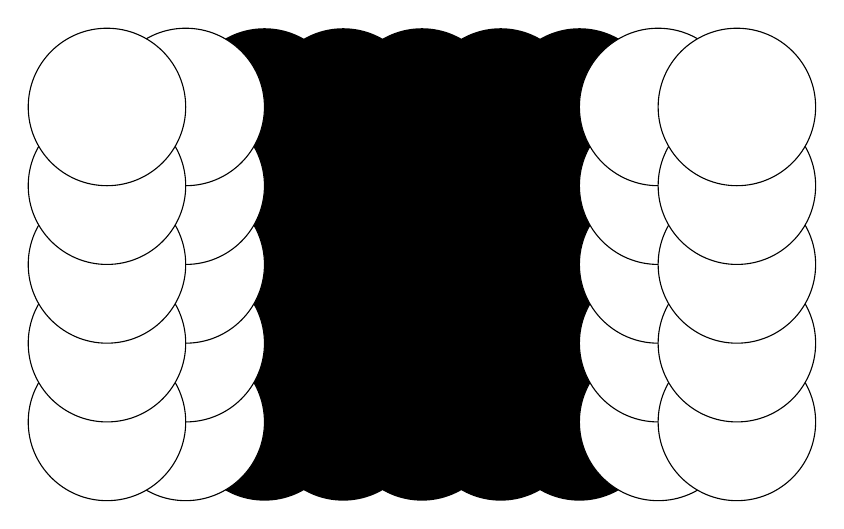
\begin{tikzpicture}
            \draw[very thin, step=1] (0,0) grid(4,4);
            \draw[very thin, dashed,step=1] (-1,0) grid(-2.5,4);
            \draw[very thin, dashed,step=1] (5,0) grid(6.5,4);
            \foreach \x in {0,...,4}{
                \foreach \y in {0,...,4}{
                    \fill (\x,\y) circle(\radius);
                }
            }
            \foreach \x in {-1,-2,5,6}{
                \foreach \y in {0,...,4}{
                    \filldraw[fill=white] (\x,\y) circle(\radius);
                }
            }

        \end{tikzpicture}
        \caption{Normally, one processor only has a local lattice and no data from the neighboring sub-lattices. An empty copy of the sub-lattice is made, to store the shifted lattice.}
    \end{subfigure}
    \begin{subfigure}{\textwidth}
        \centering
        \begin{tikzpicture}
            % Motion
            \draw[very thin, step=1] (0,0) grid(4,4);
            \draw[very thin, dashed,step=1] (-1,0) grid(-2.5,4);
            \draw[very thin, dashed,step=1] (5,0) grid(6.5,4);
            \foreach \x in {0,...,4}{
                \foreach \y in {0,...,4}{
                    \fill (\x,\y) circle(\radius);
                }
            }
            \foreach \x in {-1,-2,5,6}{
                \foreach \y in {0,...,4}{
                    \filldraw[fill=white] (\x,\y) circle(\radius);
                }
            }
            \foreach \x in {0,...,5}{
                \foreach \y in {0,...,4}{
                    \draw (\x,\y) ++(\outbend:\sepradius) coordinate(A);
                    \draw (\x-1,\y) ++(\inbend:\sepradius) coordinate (B);
                    \path[->] (A)  edge[bend right=\inbend] (B);
                }
            }
            \foreach \x in {0,4}{
                \draw (\x-\ovalspacing,-\radius) coordinate (A);
                \draw (A) ++(0,4+2*\radius) coordinate (B);
                \draw (\x+\ovalspacing,-\radius) coordinate (C);
                \draw (C) ++(0,4+2*\radius) coordinate (D);
                \draw[gray] (A) -- (B);
                \draw[gray] (C) -- (D);
                \draw[gray] (A) arc(180:360:\ovalspacing);
                \draw[gray] (D) arc(0:180:\ovalspacing);
            }
        \end{tikzpicture}
        \caption{The shifted lattice is filled with the neighboring links, some of which are received by the ``forward'' neighbor (so some are sent as well to the ``backward'' neighbor)}
        \label{subfig:shift}
    \end{subfigure}
    \begin{subfigure}{\textwidth}
        \centering
        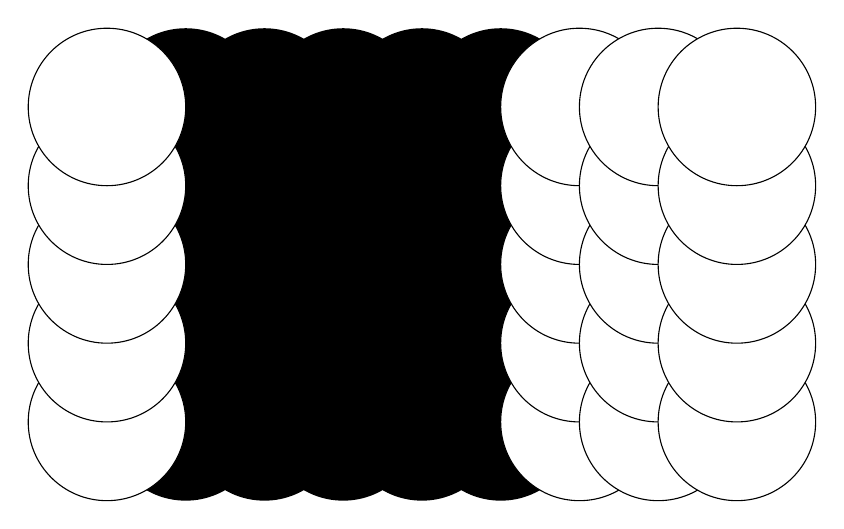
\begin{tikzpicture}
            \draw[very thin, step=1] (0,0) grid(4,4);
            \draw[very thin, dashed,step=1] (-1,0) grid(-2.5,4);
            \draw[very thin, dashed,step=1] (5,0) grid(6.5,4);
            \foreach \x in {-1,...,3}{
                \foreach \y in {0,...,4}{
                    \fill (\x,\y) circle(\radius);
                }
            }
            \foreach \x in {-2,4,5,6}{
                \foreach \y in {0,...,4}{
                    \filldraw[fill=white] (\x,\y) circle(\radius);
                }
            }
        \end{tikzpicture}
        \caption{The shifted lattice is now a local object mapped with the same indices as the original one. A site-by-site multiplication is now possible between the original and the shifted lattices.}
    \end{subfigure}
    \caption{Parallelization scheme based on lattice shifts. When, for example in the staples computation, a link needs to be multiplied by a neighboring one, a new lattice is created. It is filled with the shifted links, which are fetched either from the local sub-lattice if they are the central region, or from the neighbors they are on the edge. This schematic drawing shows how a shift along the ``right'' direction is performed. A new lattice containing the data of the target link is created by filling it with the target links. The circled regions in \cref{subfig:shift}, the edges, are shared using \texttt{MPI} by first creating a ``buffer'' of the shape of the edge (it is a cube in the real simulation) and it is sent in a single message to the neighbor which unpacks it in the right location. The new lattice is then used for arithmetical opertions with the original one on a site by site basis, which now is only a local operation.}
    \label{fig:shift}
\end{figure}

The data to be shifted is on the order of hundreds of kilobytes and sending such an amount of data using \texttt{MPI} is a time consuming operation. A possible optimization that has been implemented is to rewrite the algorithm in order to use non-blocking communications. These allow the program, while the Message Passing Interface is handling the communication, to continue with the execution instead of waiting for the message to be sent. One must however be careful not to use any of the data that is being sent or received before checking that communication has been finished. \\
In the case of lattice shifts the use of non-blocking communications is simple and highly beneficial. 
First let us recall that, because of periodic boundary conditions, sending operations are always paired to a receive one. This means that a processor sends data to its neighbor on one side and receives the corresponding data from the neighbor on the other side along the same direction (this becomes clearer by looking at \cref{fig:shift}). To start a lattice shift one first instantiates a non-blocking send instruction, then shifts the inner points of the sub-lattice (which do not require links from the neighbors) while the message is being sent. To complete the shift operation the last thing to do is to wait for the message from the neighbor from the receiving side to arrive.\\
The great reduction in communication overhead, compared to the single link exchange in \cref{sec:para_gen}, improved the scaling of the algorithm greatly, making this part of the problem much more efficient.

\subsection{Summary of the Parameters for the Gradient Flow}
As it has been done for the gauge field configuration generation algorithm, in \cref{FLOW:params} we report a summary of all free parameters of the program that performs the numerical integration of the gradient flow equation on the lattice.

\begin{table}[!htb]
\begin{center}
    \capt{Parameters for the numerical integration of the gradient flow equations \\on Yang-Mills gauge field configurations.} 
\begin{tabular}{cl}
    Parameter & Description\\\hline
    $\beta$ & Coupling parameter of the Wilson Action, fixed by the input configuration\\
    $\epsilon$ & Runge-Kutta integration step size\\
    $t_f^{MAX}$ & Maximum value of the flow time reached for every configuration. 
\end{tabular}
\label{FLOW:params}
\end{center}
\end{table} 


\section{Structure and Tools}
The programs that have been developed to genereate gauge fields and to apply the gradient flow to them have been written in \texttt{C++}. The full code can be found on the web under the link \url{https://github.com/GioPede}, where source code for both is hosted. The technical documentation is found at \url{https://giopede.github.io/LatticeYangMills/html/index.html}, but it should be noted that this is still in active development, though sufficient for this thesis, so the structure of the source code might vary from what is presented in this section. \\
The choice of programming language was mainly due to it being the most high-performing language with a high enough abstraction level. The high performance of \cpp is given by the tight link that it has to the hardware, allowing precise management of the memory and instructions optimizations. \\
One of the main features that distinguishes \cpp from the \texttt{C} programming language (a valid and equally performing alternative), is that it is an Object-Oriented language. This allows to create abstractions that give an organized structure to the source code, making the developing process easier and the code more readable and intuitive.

\subsection{Object-Oriented Programming}
One of the most successful programming paradigms is Object-Oriented Programming (OOP). An object, or ``class'', in this context is a collection of data, or ``attributes'', and procedures, ``methods'', that act on them. \\
The greatest advantage of using OOP is the introduction of an abstraction level from simple numerical variables, like integers, floating point variables or arrays, to more complex structures. A simple example of this is the class to represent $\mathrm{SU}(3)$ matrices. Instead of dealing every time with the allocation of $18$ variables ($3\times 3$ both for the real and imaginary parts) one can instantiate a variable of type \texttt{SU3}. This example is also useful to introduce the concept of operator overloading, which fundamentally means to implement mathematical operation between classes, so that objects can be used as basic elements of additions, multiplication and so on.\\
Finally, in OOP the concepts of inheritance and polymorphism are very important. The calculation of the observables is a good example for these. An observable, in the program, has a very well defined behavior and structure, for instance it stores its \texttt{value} and has a method \texttt{compute} that can be called to evaluate it given a gauge field lattice as input. However, the operations to be executed in order to compute the value depend on the observable type. An external class that wants to compute multiple observables should be able to call the \texttt{compute} method without knowing the exact type of the observable. The solution is to create an abstract base class, the observable, that only defines \texttt{value} and \texttt{compute}, but gives no specific implementation. Derived types are then created for each different type that ``inherits'' the general behavior from the base class. For an external class, the derived objects can all be used in the same way even if the exact type is unknown. The actual operations that will be performed however will depend on the derived type; this is called polymorphism.\\

\subsection{Source Code Structure}
It is possible to identify a layered structure in the class hierarchy of the program, outlined in \cref{fig:code_structure}. At the time of writing the actual design of the source-code  differs slightly from what is presented here (some classes are merged together, for example the observables), but development is being done to reach this cleaner and fully modular structure.\\

\fig[0.7]{implementation/classes.pdf}{Class structure of the code, showing the approximative hierarchy between the different components.}{fig:code_structure}

There is a set of ``Core Classes'', the second layer in figure, on top of which all the rest is built:
\begin{itemize} 
    \item the $\mathrm{SU}(3)$ matrix implementation, that specifies basic operation for the most fundamental object of Lattice QCD, the link variables. It also includes the algorithm for generating random matrices and the matrix exponential found in \cref{sec:randommatrix,sec:exponential} 
    \item the Lattice class, which specifies operations on four dimensional grids. In particular it handles most of the parallelization tools to allow distributed memory computation, like on computing clusters. The parallelization is introduced by the use of the Message Passing Interface, \texttt{MPI}, to implement for example the lattice shift function, \cref{sec:shift}.
    \item Input/Output tools, to handle input parameter files, gauge configuration parallel reading and writing, observable output files handling and standard command-line output. For the input files the choice has to write a \texttt{json} parsing class, based on the project found at \cite{_nlohmann/json}, to provide an easier user interface via the usage of a  structured input file.
\end{itemize}

With the tools described just above the main classes of the program were written. These ``Lattice Tools'', the third layer in \cref{fig:code_structure}, represent general physical concepts in Lattice QCD. They are:
\begin{itemize}
    \item the Action abstract base class, of which the Wilson Plaquette action derived type has been implemented, is an object that if given a gauge field lattice can compute: the value of the action at every single lattice site; the staples of a link (for the action derivative and the Metropolis-Hastings algorithm); the action difference of a link if provided with a random transformation for it.
    \item the Observable abstract base class. It contains simply the value of the observable and a method to compute it. The derived types that have been implemented are the Plaquette, the Energy Density and the Topological Charge.  
\end{itemize}
For both of these base classes new derived types could be implemented, extending the capabilities and the use cases of the program. \\
Finally the ``Main Applications'' that have been developed are: the Pure Gauge Field Generator, which is an implementation of the Metropolis-Hastings algorithm as presented in this chapter; the Wilson Flow, a program to apply the gradient flow equation to a set of gauge field configuration and compute observables at every flow-time; a Pure Gauge Field Reader, mainly intended for testing, it is a useful application to view the single links of a lattice configuration.
	\end{chapter}

	\begin{chapter}{Tests and Runs Description}
		\label{chap:test_runs}
		When developing a program for numerical simulations from scratch, it is crucial to design test cases and benchmarks to verify the goodness of the implementation. The easiest case is that of a fully deterministic program (for which the output depends only on some initial parameters) because one can compare the results with other implementations to validate the code. In the case of stochastic processes, for example that of a Markov chain, it is only possible to compare between different implementations the average properties and results. \\
In this chapter we will give an overview of the test cases, that determined the validity of our code; the properties of the ensembles of gauge field configurations that have been used in this thesis, and how the numerical parameters that were needed to generate them have been set.

\section{Generated Ensembles}
In order to study the scale $\Lambda_{YM}$ of Pure Yang-Mills theory it has been necessary to choose a set of decreasing lattice spacings to then be able to take the continuum limit. This procedure is common to most Lattice QCD calculations as it is the most straightforward way to recover the continuum theory. The lattice spacing is linked to the coupling $g_0$, or the inverse coupling $\beta$, by the relation found in \cref{scale:parameter}.\\ 
We chose 4 values of $\beta$ that span lattice spacings from approximately $0.1$ fm to $0.05$ fm in approximately equal steps. \\
For the calculation to be consistent however, the total volume of the lattice should be kept constant, so the choice of the lattice spacings also determined the number of lattice sites per dimension, having $L = aN\approx const$. The time dimension has been take to be twice as big as the three spatial dimensions. The number of lattice points per dimension, for the sake of parallelization, were chosen in order to have many integer divisors, to allow for many different sizes of the sub-blocks to be set. Table \cref{runs:ensembles} summarizes the physical properties of the ensembles that were generated.

\begin{table}[!htb]
    %\captionsetup{justification=centering}
    \capt{Physical properties of the ensembles used for this work. The parameter $\beta$ is the inverse coupling, and its value fixed the lattice spacing $a$ through the usage of \cref{scale:parameter}. The value of $N$ represents the number of lattice sites per spatial dimension and $N_T$, here fixed to $2N$, is the number of sites in the time dimension. The size $L = aN$ of the system is also reported, in units of fermi.}
    \begin{center}
    \begin{tabular}{cccc}
        $\beta$ & $a$ & $N^3\times N_T$ & $L$ [fm]\\\hline
        $6.00$ & $0.09314$ & $24^3 \times 48$ & $2.23536$\\
        $6.10$ & $0.07905$ & $28^3 \times 56$ & $2.21367$\\
        $6.20$ & $0.06793$ & $32^3 \times 64$ & $2.17405$\\
        $6.45$ & $0.04781$ & $48^3 \times 96$ & $2.29488$\\
    \end{tabular}
    \label{runs:ensembles}
    \end{center}
\end{table}

For each value of $\beta$ a statistical ensemble of randomly chosen gauge field configurations was needed. Ideally, one would take as many configurations as possible for each value. However it is clear from the discussion in \cref{chap:code_design} that the number of lattice sites affects computation times and the capability of storing the configurations dramatically. Moreover, as will be shown in \cref{sec:obs_autocorr} the autocorrelation time of the observables has a non-trivial, power-law or exponential behavior with the lattice spacing, making the generation of the larger $\beta$ ensembles even more challenging.\\
In \cref{runs:mcparams} we report the final values for the parameters of the Metropolis-Hastings algorithm for the different ensembles that were generated.
\begin{table}[!htb]
    \capt{Parameters used for the generation of the ensembles on which the results of this work are based on. In the table $\beta$ is the inverse coupling; ``MC Cycles'' stands for the total number of Monte Carlo updates performed, a detailed description of an update is found in \cref{sec:update}. The following parameters are the algorithm specific ones described in \cref{MC:params}.}
    \begin{center}
    \begin{tabular}{cccccc}
        $\beta$ & MC Cycles & $N_{conf}$ & $N_{corr}$ &  $N_{hit}$ & $\epsilon_{SU(3)}$\\\hline
        $6.00$ & $600000$ & $1000$ & $600$ & $30$ & $0.25$\\
        $6.10$ & $300000$ & $500$ & $600$ & $30$ & $0.25$\\
        $6.20$ & $400000$ & $500$ & $800$ & $30$ & $0.25$\\
        $6.45$ & $400000$ & $250$ & $1600$ & $30$ & $0.25$
    \end{tabular}
    \label{runs:mcparams} 
    \end{center}
\end{table}

These values have been chosen after many tests, mainly checks of the autocorrelation time of the observables presented in \cref{sec:observables}. All the parameters are free in principle and no reference study on their impact on the resulting ensemble properties was found for the case of the Metropolis-Hastings algorithm. In the next section the trial and error approach that led to he choice of these parameters will be briefly discussed.\\
Evidently, there is less freedom on the choice of the parameters in \cref{FLOW:params} for the gradient flow compared to the gauge field generation. This is because the numerical integration of the flow equation is fully deterministic. There are only two quantities to fix: the value of $t_f^{MAX}$, the final flow time point; and the size of the integration step $\epsilon$. In the calculations the flow time is expressed in lattice units, $t_f \rightarrow t_f/a^2$, so the quantities we set were in this dimensionless form. To rescale the final flow time to physical units it must be multiplied again by the square of the lattice spacing, but it is more interesting to report the final smearing radius of the flow equation, remembering that it is defined as: $\sqrt{8t_f^{MAX}}$. In \cref{runs:flow} we report the choice of the parameters for the flow of the ensembles in \cref{runs:ensembles}.
 
\begin{table}[!htb]
    \capt{Parameters used for the numerical integration of the gradient flow equations \cref{lattice:flow} for the ensembles in \cref{runs:ensembles}. The inverse coupling is $\beta$ and its value implicitly defines the lattice spacing $a$. $\epsilon$ is the size of every Runge-Kutta integration step. The value of $t_f^{MAX}/a^2$ is the last point of integration in dimensionless units and the corresponding maximum smearing radius is shown as  $\sqrt{8t_f^{MAX}}$ in fermi.}
    \begin{center}
    \begin{tabular}{cccc} 
        $\beta$ & $\epsilon$ & $t_f^{MAX}/a^2$ & $\sqrt{8t_f^{MAX}}$ [fm] \\\hline
        $6.00$ & $0.01$ & $10.00$ & $0.8330$ \\
        $6.10$ & $0.01$ & $10.00$ & $0.7070$ \\
        $6.20$ & $0.01$ & $10.00$ & $0.6076$ \\
        $6.45$ & $0.02$ & $20.00$ & $0.6047$ 
    \end{tabular}
    \label{runs:flow} 
    \end{center}
\end{table}
The choice of $\epsilon$ was motivated by the work by C\`{e} et al. \cite{ce_testing_2015}, and the same values for the combination of $\epsilon$ and $t_f^{MAX}/a^2$ have been chosen for all ensembles, regardless of the physical maximum smearing radius. The exception is the $\beta=6.45$ case, for which the total number of integration steps of the Runge-Kutta Munthe-Kaas integrator has been kept equal to the other lattice sizes, but the integration step length is doubled. This was needed to obtain results for large enough smearing radii out of the ensemble (which is by far the largest one) in reasonable computing time.


\section{Test Runs}
\label{sec:testautocorr}
Running some test calculations with a completely new program is obviously necessary. The simplest benchmark was to check the expectation values of the observables. To perform these checks we computed the energy density and the topological charge on two configurations generated with the CHROMA lattice QCD code from the USQCD collaboration\cite{edwards_chroma_2005}.  The results were found to match to machine precision. \\
The gradient flow implementation could also be tested numerically by comparing our results to the ones generated by an extension of CHROMA called FlowOps (courtesy of T.Luu and A.Shindler)\cite{shindler_nucleon_2015}. This program as well applies the gradient flow to gauge field configurations with the same integrator scheme that we used, \cref{eq:integrator}, thus by setting the same integration parameters we were able to compare the values of the observables at every flow time. Also in this case our implementation gave results equal to machine precision to the ones by FlowOps at all flow times for every configuration we tested.\\
Checking the validity of expectation values of observables is a solid indication that the overall core libraries of the new framework we developed has been implemented correctly. \\
Testing the algorithm to generate gauge field configurations and assessing the quality of the generated ensembles is much harder than testing the gradient flow, because it involves stochastic computations, hence no numerical check can be easily defined. One has instead to look at average properties of the set of configurations. The generation of gauge field configurations as we saw in \cref{MC:params} has three parameters that need to be set that do affect the statistical properties of the output ensemble, mainly the autocorrelation time of the observables. The simplest parameter to set was $\epsilon_{\mathrm{SU}(3)}$, which controls the spread of the $\mathrm{SU}(3)$ random elements around the identity matrix. This directly affects how much each link is changed from one MC cycle to the other, a larger value of $\epsilon_{\mathrm{SU}(3)}$ implies larger changes. The drawback is the decrease of the acceptance ratio of the Metropolis test and consequently of the efficiency of the program. The value that was chosen, $0.25$ was a good trade-off between the two things.\\
The other parameters two parameters to set were: $N_{corr}$, the number of configurations between observable measurements (in parctice between two saved configurations); ($N_{hits}$ the number of random unitary transformations applied to every link per MC cycle. Some tests runs with different combinations of the two were performed on the three largest lattice spacings, as the system for the smallest one is much larger and requires a considerably longer time to compute.


\subsection{Tests for the Autocorrelation of Observables}
\label{sec:obs_autocorr}
The most important test has been the assessment of the autocorrelation time for different observables at various lattice spacings varying the parameters of the ensemble generation algorithm. As expected, the most problematic quantity is the topological charge, especially at large flow times. A good measure of how much a data series is autocorrelated is the integrated autocorrelation time $\tau_{int}$, see \cref{app:autocorr}, which is expected to be $1/2$ if the data is uncorrelated. In general, a larger $\tau_{int}$ implies an underestimation of uncertainties, so the variance of a quantity is corrected as $\tilde\sigma^2 = 2\tau_{int}\sigma^2$. \\
The first test, in \cref{fig:autobetas} shows the integrated autocorrelation time for the topological charge at fixed $N_{corr}=200$ and $N_{hit} = 10$ for different lattice spacings:
\fig[0.7]{implementation/TopcAutoBetas.pdf}{Integrated autocorrelation time $\tau_{int}$ of the topological plotted against the smearing radius of the gradient flow $\sqrt{8t_f}$. The different ensembles shown have fixed values of $N_{corr}=200$ and $N_{hit} = 10$ and the different data series represent increasing values of the inverse coupling. The system sizes are the ones of \cref{runs:ensembles} for every value of $\beta$. }{fig:autobetas}

From the plot it is clear that the values that were guessed for the parameters $N_{corr}$ and $N_{hit}$, which could be acceptable for the lowest beta value, are not at all fine for the other lattice spacings. One can observe that for increasing values of $\beta$ the $\tau_{int}$ grows rapidly if the parameters of the generation algorithm are kept fixed.  This is the reason why in \cref{runs:ensembles} the different ensembles have different parameters, in particular growing $N_{corr}$ which represents the number of MC updates between two measurements of the  observables.\\
On a general note we see how the flow quickly removes the low range noise from the observable through the smearing effect, making it clear that the topological charge is highly correlated in Monte Carlo time even though it might seem uncorrelated if one only looks at $t_f = 0$. \\
A second test was to look at a single lattice spacing and try to vary the parameters $N_{corr}$ and $N_{hits}$. The results for the $\beta=6.10$ case are shown in . 
\fig[0.7]{implementation/TopcTauInt.pdf}{Integrated autocorrelation time of the topological charge as a function of the smearing radius of the gradient flow $\sqrt{8t_f}$. The ensembles have been generated with inverse coupling $\beta=6.10$ for a lattice of size $28^3\times58$. The different data series represent different combinations of the parameters for the gauge field generation $N_{corr}$ and $N_{hit}$. The black data series shows the set of parameters that were chosen for the generation of the larger ensemble (the one used for the analysis of the energy scale $\Lambda_{YM}$). }{fig:autotauint}
\\
The results of \cref{fig:autotauint} suggests a possible cure for the autocorrelation of the observables. It is almost tautological that increasing the value of $N_{corr}$ decreases the integrated autocorrelation time, as the parameter represents how many MC updates are performed between two measurements of the observable. The dependence of $\tau_{int}$ from $N_{hits}$ is also clear since the more attempts of transforming a single link are performed, the more the configuration will be different from the previous one. \\
From the plot we can observe that increasing both parameters decrease $tau_{int}$, so the choice was to set both to a larger value from our initial guesses. This proved to be the right choice. \\
The black data series in  \cref{fig:autotauint} is the data that we used for our analysis. One can notice that it is still autocorrelated, but to a degree that can be handled with a reasonable correction to the variance of the data. \\
It is important to stress again that autocorrelation is a huge problem mainly for the topological charge. The energy density operator is much less affected and for all the ensembles we generated the integrated autocorrelation time is never a value much greater that $1/2$ (see \cref{fig:energyautocorr}). 


\subsection{Thermalization}
\label{sec:thermalization}
When computing expectation values using Monte Carlo integration, it is important to ensure that the sampling of the observables is performed when the Metropolis-Hastings algorithm reached equilibrium, or in jargon when it is thermalized.\\
The Markov Chain to generate gauge field configurations can be initilized in two distinct ways. These represent the initial configuration of the gauge field to which Monte Carlo updates are later applied. The two possibilities are:
\begin{itemize} 
    \item Cold Start: all links of the gauge field configuration are set to the $\mathrm{SU}(3)$ identity element;
    \item Hot Start: all links are set to random $\mathrm{SU}(3)$ matrices.
\end{itemize}
It is easy to see that for the cold start the initial value for the plaquette operator, \cref{plaquette}, would be one, when normalized on the lattice volume and so the action starts in its minimum. For the hot start the initial value for the plaquette expectation value is a random number, centered around zero. The Metropolis-Hastings algorithm is supposed to drive the Markov chain towards the peak of the PDF, \cref{eq:PDF}, that corresponds to an intermediate value of the two. \\
\fig[0.7]{implementation/ThermPlaq.pdf}{Expectation value of the Plaquette as a function of the number Monte Carlo cycles performed, for hot and cold starts. Equilibrium is reached in both cases after $\approx 600$ updates. The data is taken from a simulation with $\beta=6.10$.}{fig:thermalization}

In \cref{fig:thermalization} we show that only a small number of MC updates is needed to reach equilibrium, especially when compared to the value of $N_{corr}$ from the discussion in \cref{sec:obs_autocorr}. \\
To ensure thermalization, all results of this work are generated discarding the first $10^4$ MC cycles, which is much larger than the value we found, but still a small fraction, so an affordable exaggeration, of the total number of MC cycles of the Markov chain.

\subsection{Strong and Weak Scaling}
One important thing to look at when developing a program intended to be highly parallelized are the scaling properties. We can now check these for the two sections of the code, the generation of configurations and the gradient flow. We will distinguish the analysis in the two usual quantities used in High Performance Computing: strong and weak scaling. \\
\subsubsection{Strong Scaling}
Strong scaling is the performance of a program as the total problem size is kept fixed and the number of parallel units, the number of processors in this case, increases. The parallel efficiency is computed as:
\beq
    \eta_s = \frac{t_0}{t_NN}\cdot 100\% 
    \label{eq:eta_strong}
\eeq 
where $t_0$ is the execution time for one unit of computation, $t_N$ the execution time for the case of $N$ units computing the same system size. In the case for perfect parallelization the efficiency is $100\%$ as an increase of some factor in the number of processors would decrease by the same factor the execution time. In real cases this is seldomly true, the execution time is in fact usually larger than expected. \\
The test was set up in this way:
\begin{itemize}
    \item Gauge Field Generation: one lattice of size $24^3\times 48$ has been randomly generated and $10^4$ MC cycles were performed. The system was split in sub-lattices of decreasing size, in order to increase the number of processors.
    \item Gradient Flow: ten lattices of size $24^3\times 48$ have been flowed for a total of $1000$ integration steps each. Again, the sub-lattice size was decreased and the number of processor increased accordingly. 
\end{itemize}

\fig[0.7]{implementation/StrongScaling.pdf}{Strong scaling of the two parts of the program. The efficiency, \cref{eq:eta_strong}, is normalized to the first point plotted, that is 64 processors.}{fig:strong_scaling}

Figure \ref{fig:strong_scaling} shows that the performance scales well with the number of processors, but the efficiency is dropping for large processor numbers. This is expected and the reason is that the surface to volume ratio of the sub-lattice decreases when more processors are added. This makes the fraction of operations that require inter-processor communication become comparable to the ``inner" points calculations. It is to be noted that smaller number of processors could not be used, as the processors in that case would have been all on the same node (the cluster used for testing has 28 cores per node), so any timing would have excluded the inter-node communication time, which is significantly higher than the inter-node one.\\
Overall the gradient flow program scales better than the ensemble generation one. This is most likely explained by the fact that the communication overhead introduced by \texttt{MPI} is larger in the case of the generation program (which shares one link variable at a time) than in the gradient flow code (which uses lattice shifts and shares one whole shared edge between processors at once, see \cref{sec:shift} for details).

\subsubsection{Weak Scaling}
By weak scaling of a parallelized problem it is intended the measure of the performance as the local workload is kept fixed and the total volume of the problem is increased by adding processors. The efficiency is computed as:
\beq
\eta_W = \frac{t_0}{t_N}\cdot 100\% 
\label{eq:eta_weak}
\eeq 
where $t_0$ is the execution time of the smallest case and $t_N$ the one of a system $N$ times larger computed on $N$ times the parallel units. The test setup was:
\begin{itemize}
    \item Gauge Field Generation: the sub-lattice has been fixed to $4^4$, and volumes from $16^3\times32$, a total of $32$ processes, to $32^3\times64$, $512$ processors, have been considered. Intermediate volumes are built by multiplying one spatial dimension at a time by a factor of 2. For each volume $10000$ MC cycles have been computed.
    \item Gradient Flow: the gauge fields generated in the previous point have been flowed for a total of $1000$ integration steps by the same number of processors that generated them, so the sub-lattice size was set again to be $4^4$.
\end{itemize}

\fig[0.7]{implementation/WeakScaling.pdf}{Weak scaling of the two parts of the program. The efficiency is the ratio of \cref{eq:eta_weak} with respect to the first data point. }{fig:weak_scaling}

The results in \cref{fig:weak_scaling} show that both the programs are perfectly scalable. The communication overhead, introduced by the need of sharing link variables across the edges, is almost constant with respect to the number of processors. We should note that already the first point plotted contains a large amount of communications between processors. What the plot is truly suggesting is that the addition of other processors keeps the overall overhead constant. This implies that the parallelization procedure has been implemented correctly, though it could still be potentially improved by further optimizations.

These results for strong and weak scaling are very comforting, as they show that the hardest part of the development process, the parallelization of the code, has been well designed and implemented.


\section{Main Runs and Timing}
To generate all the data that was needed for our analysis we had to perform eight main calculations. First we generated the four ensembles of table \cref{runs:ensembles}, by running the gauge field generator code. Afterwards the numerical integration of the gradient flow equation has been performed on all the four sets of gauge field configurations.\\
All runs of the programs, were carried out on the High Performance Computing Center at Michigan State University (MSU), with the support of the Institute for Cyber-Enabled Research (iCER). Development was performed on local machines and on the small cluster SMAUG located at the Department of Physics of the University of Oslo (UiO) and some larger benchmarks were run on the Abel Computer Cluster also at UiO.\\
The ensembles on which the results in \cref{part:results} are based were generated using the parameters in  \cref{runs:mcparams}. A summary of the computational resources used for the generation of all four ensembles is presented in \cref{runs:times}. 

\begin{table}[!htb]
    \capt{Execution times for generating ensembles from \cref{runs:ensembles} with parameters found in \cref{runs:mcparams}. All the runs were performed on the iCER cluster at MSU. $N_{procs}$ is the number of processors used for each ensemble; the Wall Time is the ``wall clock'' time (the time spent in the parallel execution); Time per MC cycle is the time spend in each step of the Markov Chain; Time per Configuration is the time spent between saved configurations, to be used for observables, so it includes the adjustment made for the longer autocorrelation times of larger $\beta$ values.} 
    \begin{center}
    \begin{tabular}{ccccc}
        $\beta$ & $N_{procs}$ & Wall Time [h] & Time per MC Cycle [s] & Time per Configuration [s]\\\hline
        $6.00$ & $1024$ & $27$ & $0.16104$  & $96.6$\\
        $6.10$ & $512$ & $35$ & $0.42102$ & $252.6$\\
        $6.20$ & $1024$ & $53$ & $0.4780825$ & $382.4$ \\
        $6.45$ & $1024$ & $204$ & $1.836$ & $2937.6$
    \end{tabular}
    \label{runs:times} 
    \end{center}
\end{table}

It is clear from the table that the $\beta=6.45$ ensemble, out of which only 250 configurations were saved, had execution times larger by one order of magnitude compared to the second largest; this made increasing the ensemble size unfeasible with the time and resources for this work.\\
To conclude, in \cref{runs:times_flow} we present the summary of the computational resources used by the Gradient Flow program to integrate the flow equation on all the configurations of the ensembles.

\begin{table}[!htb]
    \capt{Execution times for the numerical integration of the flow equations on the ensembles from \cref{runs:flow} with parameters found in \cref{runs:flow}. All the runs were performed on the iCER cluster at MSU. $N_{procs}$ is the number of processors used for each ensemble; the Wall Time is the ``wall clock'' time (the time spent in the parallel execution); Time per Configuration is the time spent flowing one single gauge configuration.} 
    \begin{center}
    \begin{tabular}{cccc}
        $\beta$ & $N_{procs}$ & Wall Time [h] & Time per Configuration [s]\\\hline
        $6.00$ & $1024$ & $15$ & $109.3$\\
        $6.10$ & $512$ & $30$ & $218.6$\\
        $6.20$ & $1024$ & $33$ & $243.6$ \\
        $6.45$ & $1024$ & $96$ & $1326.9$
    \end{tabular}
    \label{runs:times_flow} 
    \end{center}
\end{table}
  \end{chapter}
\end{part}


% PART III: RESULTS
\begin{part}{Data Analysis and Results}
	\label{part:results}
	\begin{chapter}{Raw Observables}
  		\label{chap:obs_results}
  		In this chapter the results for simple expectation values computed on the lattice gauge field ensembles that have been generated for this work, \cref{runs:ensembles}, are presented. Throughout the chapter, all error estimates associated to expectation values of observables have been computed using the bootstrap method, see \cref{app:resampling}, which is a popular resampling method used when the sample size of a statistical population is small, as is our case. The autocorrelation of data from the ensembles, introduced by the use of Markov chain to generate it, is handled using the procedure found in \cref{app:autocorr} as a correction to the estimate of the variance proportional to the integrated autocorrelation time.

\section{Plaquette and Energy Density} 
The plaquette, \cref{plaquette}, and the energy density, \cref{eq:energy}, are tightly related as they both are estimates of the action of the gauge field.
%  We have already seen in \cref{sec:thermalization} that the plaquette can be used to check whether the metropolis algorithm has thermalized in the early stages of the chain. One could also study the dependence of the plaquette expectation value on the inverse coupling $\beta$ of the gluonic action. In \cref{fig:betplaq} the average plaquette computed for different inverse couplings. 
% \fig[0.7]{results/BetaPlaq.pdf}{Average Plaquette value as a bunction of the inverse coupling $\beta$.}{fig:betplaq}
Since the system is expected, after thermalization, to be at equilibrium, the sampling of the plaquette and of the energy density should be rather constant. To test this we can look, for example, at the value of the observables computed on a single gauge field configuration and plot them in the order in which they were generated, \ref{fig:MCPlaqEnerg}. This is often referred to as the ``Monte Carlo history'' of the observable.
\begin{figure}[hbt!]
    \centering
    \begin{subfigure}{0.45\textwidth}
        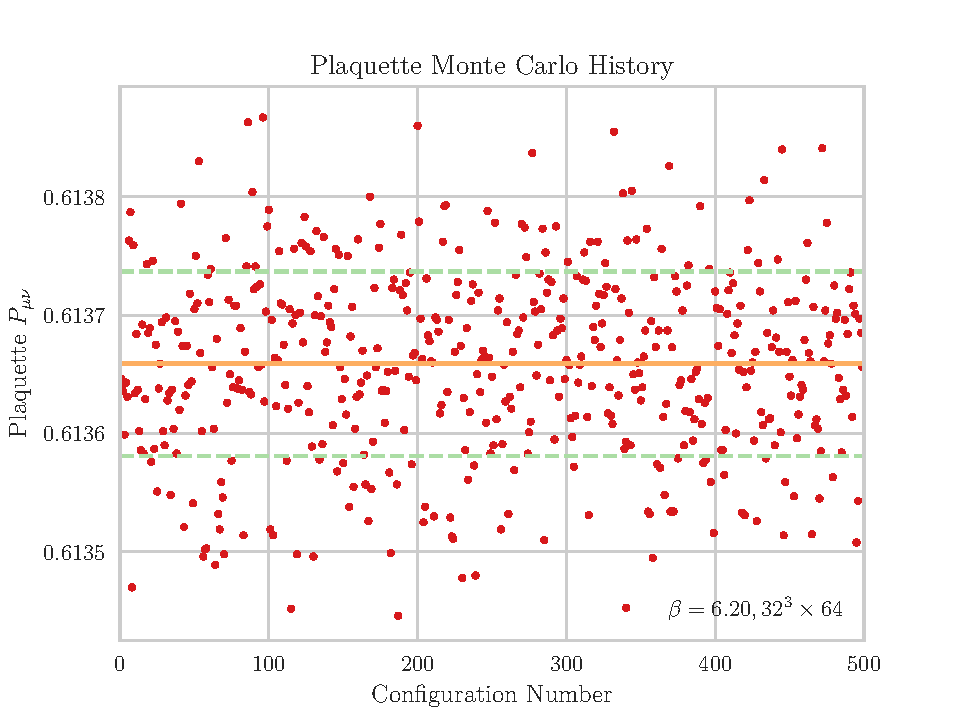
\includegraphics[width=\textwidth]{results/MCPlaq.pdf}
    \end{subfigure}
    \begin{subfigure}{0.45\textwidth}
        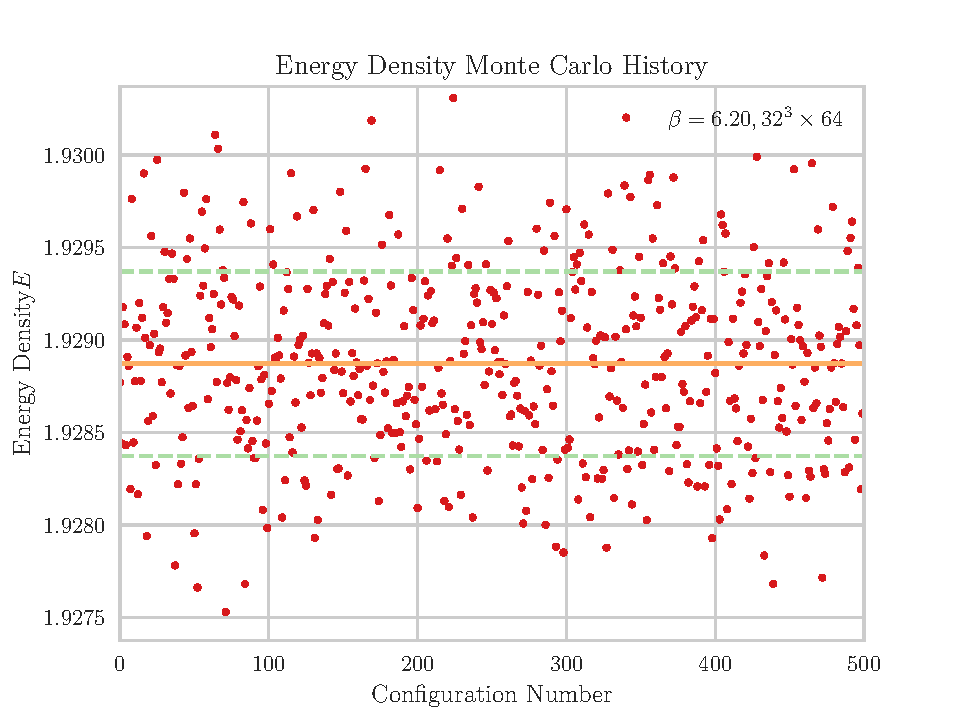
\includegraphics[width=\textwidth]{results/MCEnrg.pdf}
    \end{subfigure}
    \caption{\footnotesize Values for the Plaquette (left) and Energy Density (right) as a function of Monte Carlo time. The blue line is the average and the green dashed lines are the one $\sigma$ interval around it. The points represent the values of the two observables computed on every configuration of the ensemble. The average is thus the expectation value.}
    \label{fig:MCPlaqEnerg}
\end{figure}   

When applying the gradient flow equation:
\beq
\partial_{t_f} V_{t_f}(x,\mu) = - g_0^2 [\partial_{x,\mu}S_G(V_{t_f})]V_{t_f}(x,\mu),
\eeq
the configuration is evolved towards the minimum of the action. That implies that the values for the plaquette and the energy density at sufficiently large flow times are both lattice spacing and flow time independent. The results plotted in \cref{fig:plaq_plot} for the plaquette expectation value as a function of flow time, show that the gradient flow is indeed driving the gauge fields towards the stationary points. From the expression of the Wilson gluonic action, \cref{wilsonaction}, it is clear that the minimum of the action is reached when all the plaquettes are equal to the identity matrix. 
The expectation value of the average plaquette is therefore expected to be exactly one. 
\fig[0.7]{results/Plaquette.pdf}{Plaquette expectation value $\langle P_{\mu\nu} \rangle$ as a function of flow time $t_f$, here expressed in the form of the smearing radius $\sqrt{8t_f}$. The data for all the four ensembles of \cref{runs:ensembles} is shown. Error bars are too small to be visible on the plot.}{fig:plaq_plot}\\
The energy density has an even simpler proportional relation to the action and \cref{fig:energy_plot} proves that the action is indeed minimized in the large flow time limit.
\fig[0.7]{results/Energy.pdf}{Energy density expectation value $\langle E\rangle$ as a function of gradient flow smearing radius $\sqrt{8t_f}$. The different data series represent the four different ensembles that have been generated, see \cref{runs:ensembles}. The error bars are not visible on the plot as they are small.}{fig:energy_plot}\\
As discussed in \cref{sec:obs_autocorr}, the integrated autocorrelation time of the observables is a crucial quantity to assess the quality of the results. We therefore computed $\tau_{int}$ for the energies for all the different ensembles at all flow time values. From \cref{fig:energyautocorr} we conclude that for all ensembles we generated the value of $\tau_{int}$ for the energy density never exceeds the value of one at any flow time. This result is suggesting that the data we sampled for this observable is almost uncorrelated. Nevertheless, all results of this work (including \cref{fig:plaq_plot} and \cref{fig:energy_plot}) have variances corrected by $\tilde\sigma^2 = 2\tau_{int}\sigma^2$. The discontinuities in the integrated autocorrelation time stem from different truncations in the windowing procedure described in \cref{app:autocorr}. One can however notice that the values between the jumps are still compatible within the error estimate of $\tau_{int}$ given by \cref{eq:tauint_error}. 
\fig[0.7]{results/EnergyTauInt.pdf}{Integrated autocorrelation time of the Energy Density as a function of the smearing radius $\sqrt{8t_f}$. The discontinuity of the data is given by the approximation given by the truncation procedure described in \cref{app:autocorr}. The method to compute the error bars on $\tau_{int}$ is also found in the same appendix.}{fig:energyautocorr} 
\section{Topological Charge}
Another interesting quantity to compute on our gauge fields is the topological charge, as defined in \cref{eq:topc}. In the continuum theory it assumes only integer values, with a distribution around zero that resembles a gaussian, though there are studies that prove that indeed it is not a normal distribution \cite{ce_non-gaussianities_2015}. \\
The topological charge on the lattice is affected by short range fluctuations given by discretization effects. The smoothing properties of the gradient flow on this observable removes the fluctuations and reveals the ``true'' value of the charge. An illustrative example is to plot the topological charge of one gauge field configuration as a function of the smearing radius. In \cref{fig:topcsingle} we show the evolution of the topological charge for three different gauge field configurations of lattice spacing $a=0.049$ fm ($\beta=6.45$). 
\fig[0.7]{results/TopcSingle.pdf}{Topological charge for three single gauge field configurations, taken at random from the $\beta=6.45$ ensemble, plotted against the smearing radius $\sqrt{8t_f}$ of the gradient flow.}{fig:topcsingle}

We can notice that for all the three considered configurations the topological charge has a plateau at a smearing of roughly $0.15$ fm. The value, for this example, corresponds to approximately three times the lattice spacing.\\ 
For some configurations however, especially for larger lattice spacings, the plateau is not clear and defined. The explanation could be the too simple definition that has been used for the gauge field strength tensor. Perhaps an improved definition of the tensor, given for example by a linear combination of plaquettes and larger Wilson Loops could be beneficial \cite{bilson-thompson_highly-improved_2003,alexandrou_comparison_2017}. These higher order definitions of $G_{\mu\nu}(n)$ can be systematically constructed to cancel the $\mathcal{O}(a^2)$ errors that we have in the current definition. A simple example is to include Wilson loops of size $1\times1$ (the plaquettes),  $2\times1$ and $1\times2$ (minimal rectangles). The topological charge density would then become:
\beq
    q^{imp}(n) = \frac{1}{32\pi^2} c_0 \epsilon^{\mu\nu\rho\sigma}\Tr [G_{\mu\nu}^{(clover)}(n)G_{\rho\sigma}^{(clover)}(n)] + c_1 \epsilon^{\mu\nu\rho\sigma}\Tr [G_{\mu\nu}^{(rect)}(n)G_{\rho\sigma}^{(rect)}(n)],
\eeq
where $G_{\mu\nu}^{(rect)}(n)$ represents the sum of all Wilson loops in the plane $\mu\nu$ of side 2. The coefficients $c_0$ and $c_1$ are set by looking at the expansion of $G_{\mu\nu}^2(x)$ on the lattice. This potential improvement could be a future addition to our program.

When considering the expectation value of the topological charge of an ensemble, we expect its value to be zero \cite{ce_non-gaussianities_2015}. From \cref{fig:topc} one can check that our data for the expectation value of $\langle Q\rangle$ is in fact within error-bars always compatible with zero. 
\fig[0.7]{results/TopChar.pdf}{Topological charge expectaion value $\langle Q\rangle$ as a function of the smearing radius $\sqrt{8t_f}$. Error bars are computed using bootstrap and corrected with the integrated autocorrelation time correction factor.}{fig:topc}

We should note that the increasing error-bars, for $\beta = 6.2$ and $\beta = 6.45$ in particular, are given by the decreasing lattice spacing. The autocorrelation time of the topological charge increases non linearly with the spacing, so the variance, which we correct according to \cref{eq:tauint}. Another reason for the larger uncertainty is the smaller ensemble size, which for the $\beta = 6.45$ contains a quarter of the gauge fields of the  $\beta=6.00$  case. \\
In \cref{fig:topctauint} we plot the integrated autocorrelation time of the topological charge as a function of flow time. If compared to the analog plot for the energy density (\cref{fig:energyautocorr}) one can notice that the two observables have very different autocorrelation times. The topological charge not only has a much larger $\tau_{int}$ on the lattice, but it grows rapidly with the inverse lattice spacing. It should be noted that the value of $N_{corr}$, the Monte Carlo updates between two data points, is much larger for the $\beta=6.45$ ensemble than all the others, but nevertheless the $\tau_{int}$ is by far larger.
\fig[0.7]{results/TopcTauInt.pdf}{Integrated autocorrelation time $\tau_{int}$ of the topological charge as a function of the gradient flow smearing radius $\sqrt{8t_f}$. The ensembles are the ones reported in \cref{runs:ensembles}. The integrated autocorrelation time and its error bars are computed using the procedure found \cref{app:autocorr}.}{fig:topctauint}

One last consideration on the topological charge is the comparison of its distribution at zero flow time and the one in the large flow time limit. In \cref{fig:topchist} we show two histograms of such distributions for the $\beta = 6.20$ ensemble at $\sqrt{8t_f} = 0$ fm and $\sqrt{8t_f} = 0.6$ fm respectively. The bins are taken to be centered on integer and half-integer values in order to capture differences of the distribution of the topological charge. In the continuum, only integer values should be allowed, while on the lattice, due to discretization, the topological charge is in general not an integer. However, from \cref{fig:topchist} it is possible to see that the gradient flow estimate of the charge has a distribution with much sharper peaks around integer values, rather than half-integer ones, if compared to the zero flow time distribution. 
\begin{figure}[hbt!]
    \centering
    \begin{subfigure}{0.7\textwidth}
        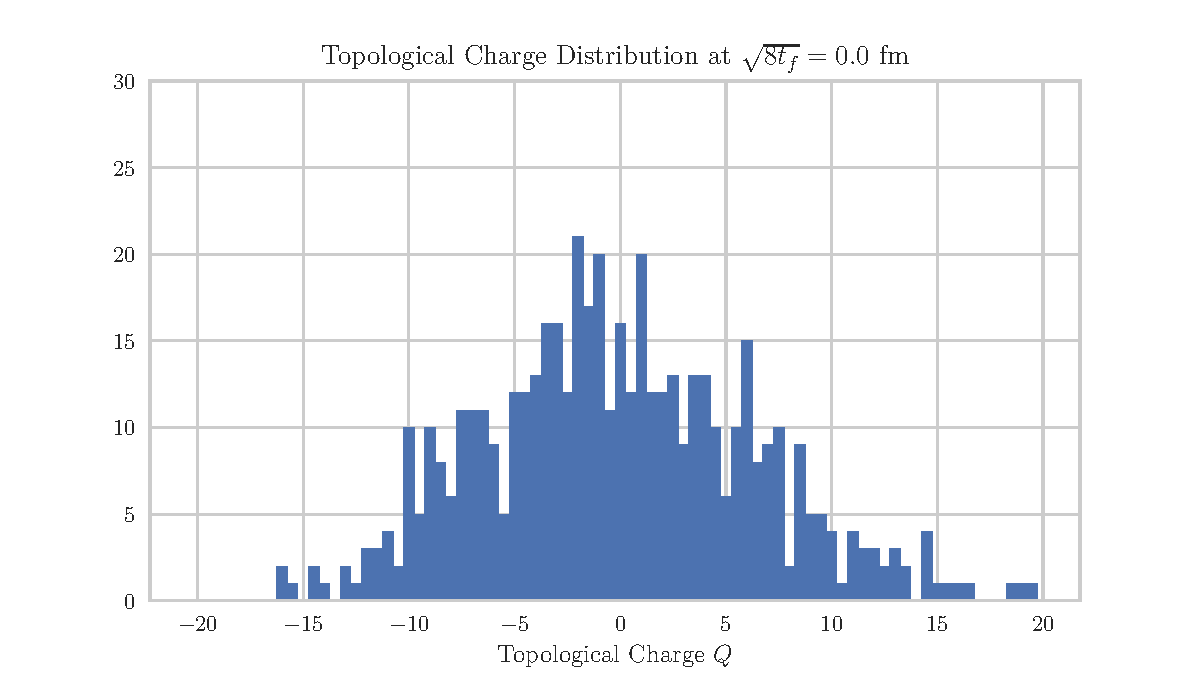
\includegraphics[width=\textwidth]{results/TopcHistNoFlow.pdf}
    \end{subfigure}
    \begin{subfigure}{0.7\textwidth}
        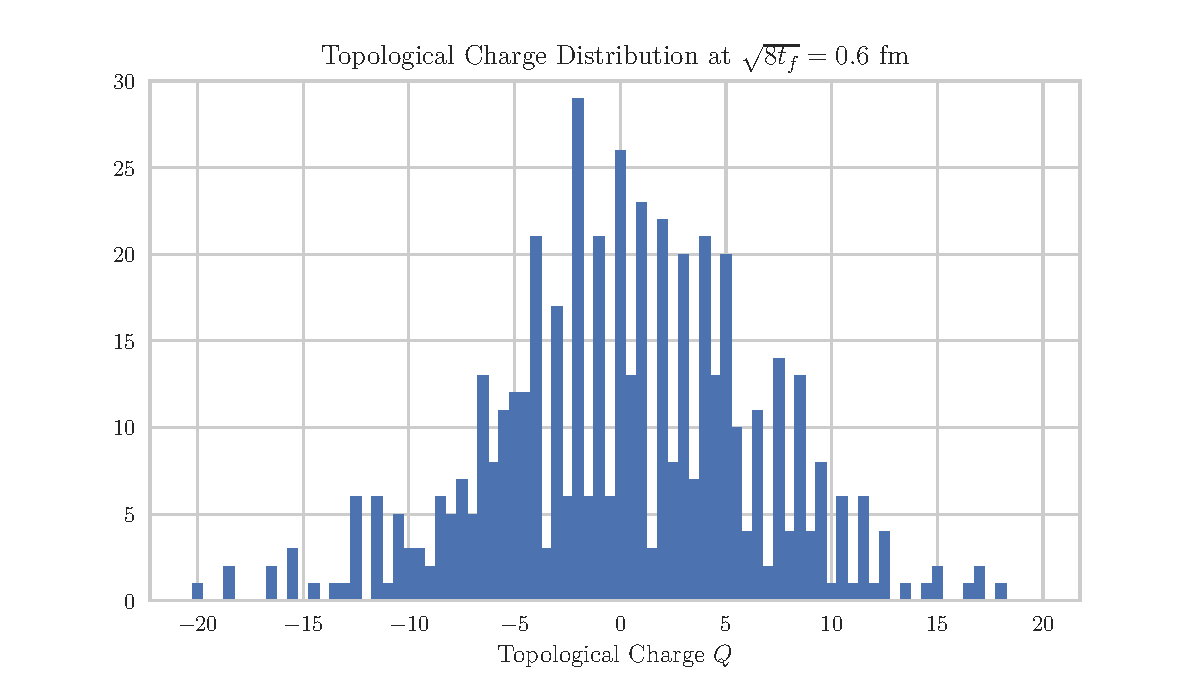
\includegraphics[width=\textwidth]{results/TopcHistFlow.pdf}
    \end{subfigure}
    \caption{\footnotesize Histograms of the topological charge values at $\sqrt{8t_f} = 0$ fm (top) and $\sqrt{8t_f} = 0.6$ fm (bottom) for the $\beta=6.20$ ensemble. The bins are centered on integers and half-integer values.}
    \label{fig:topchist}
\end{figure} 

\section{Topological Susceptibility}
The last physical quantity we present in this chapter is the topological susceptibility, \cref{eq:topsus}. Being proportional to the expectation value of the squared topological charge, it is related to the width of the distributions in \cref{fig:topchist}. The evolution with the gradient flow of the susceptibility is not trivial. At large flow times the smoothing property of the gradient flow removes the discretization effects and the real value of the quantity emerges. In \cref{fig:tops} the flow time evolution of the topological susceptibility is shown.
\fig[0.7]{results/TopSusc.pdf}{Topological susceptibility $\chi^{1/4}$ as a function of the smearing radius $\sqrt{8t_f}$, for all the ensembles generated for this work.}{fig:tops} 
 
The value of $\chi^{\frac{1}{4}}$, as defined in \cref{eq:topsus} has the physical units of energy, hence it is reported in MeV. We notice that for all ensembles in the large flow time limit the topological charge has a well defined plateau. \\
The behavior at zero flow time is not what we were expecting, comparing for example to ref. \cite{shindler_nucleon_2015} we don't observe a clear divergency at $\sqrt{8t_f} = 0$ fm for small values of $\beta$. The behavior seems to be more and more divergent (a true divergency is impossible, it is always a finite quantity on the lattice) for larger values of $\beta$. This is because the short-range effects are more pronounced for smaller lattice spacings. A possible explanation for the difference in our results compared to \cite{shindler_nucleon_2015} is the usage of the clover definition of the gauge field strength tensor. Being the topological charge, at zero flow time, dominated by short-distance fluctuations, the use of only $1\times1$ Wilson loops (the four plaquettes of the clover, \cref{fig:clover}) in the definition of $G_{\mu\nu}$ could be a problem. In the reference \cite{shindler_nucleon_2015} the field strength tensor was computed including loops up to size three, this could be the cause of the difference in the low-flow time behavior. This dependence at small flow time of the susceptibility on the definition of the field strength tensor should be investigated more. \\
From \cref{fig:tops} one can infer that the continuum limit, to recover the physical value of the topological susceptibility, can be taken by considering the value of the observable over an interval of the smearing radius between  $\sqrt{8t_f} = 0.4$ and $0.6$ fm. In principle the continuum limit could be taken at any point for the flow time. However, large discretization effects would appear at small flow time. In practice it is easier to extrapolate to the continuum in regions where all the different data series (one for each lattice spacing) have become constant. \\
In our case the extrapolation to the continuum has to be performed by using the dimensionless quantity $(a/r_0)^2$, with $a$ being the lattice spacing and $r_0 = 0.5$ fm the Sommer parameter \cite{guagnelli_precision_1998}. The ratio is taken squared in order to match the order of the discretization effects of the quantity that is being extrapolated, the susceptibility in this case. In \cref{fig:topscontlimit} the continuum limit of the topological susceptibility is taken using the values found for $\sqrt{8t_f}=0.5$ fm.   

\fig[0.7]{results/TopsContLimit.pdf}{Continuum limit extrapolation of $\chi^{\frac{1}{4}}$ from the values at $\sqrt{8t_f}=0.5$ fm. The fit is performed using the dimensionless quantity $(a/r_0)^2$ as a reference scale. The red line and the red errorband represent the fit on all the points and its $1\sigma$ confidence interval. The black point is the extrapolated point from this fit. The green line and its associated errorband are the result of fitting only the three smallest lattice spacings.  The dark green point is the continuum limit extrapolation of the latter fit.}{fig:topscontlimit}

The value we obtain for the extrapolated topological susceptibility is:
\beq
    \chi^{\frac{1}{4}} = 186.9(8.6)~\text{MeV} .
    \label{val:tops}
\eeq 
This is compatible with the value in \cite{shindler_nucleon_2015} of  $\chi^{\frac{1}{4}} = 195.9(4.9)~\text{MeV} $ and with that of \cite{ce_testing_2015} reported as $\chi^{\frac{1}{4}} = 185(5)$. However, from \cref{fig:topscontlimit} one can notice that the result highly depends on the choice of the fit. If the coarsest lattice is neglected the extrapolated value for the topological susceptibility becomes $\chi^{\frac{1}{4}}= 171.7(9.8)~\text{MeV}$. This value, even if still compatible with the previous one shows that there is a systematic uncertainty given by the choice of the fit domain. The  dependence of the topological susceptibility on the definition of the topological charge and a better assessment of the systematic uncertainties of the continuum limit extrapolation are the current study of a future master thesis by H.M. Vege. 

As an additional result we can use this extrapolation to compute the mass of the $\eta'$ meson taken from the Witten-Veneziano formula \cite{witten_current_1979}:
\beq
    \chi = \frac{F_\pi^2m_{\eta'}^2}{2N_{flavors}}.
\eeq 
Using as inputs $F_\pi = 92$ MeV, the pion decay constant, and having $N_{flavors} = 3$, we find the mass of the $\eta'$ meson to be:
\beq    
    m^{(lattice)}_{\eta'} = \sqrt{\frac{\chi 2N_{flavors}}{F_\pi^2}} = 930(27)~\text{MeV},
\eeq
which we compare with the experimental value  $m^{(exp)}_{\eta'} = 957.78(6)$ MeV \cite{dissertori_9._2016}. Our results is in agreement with the reference, but this does no mean the calculation is valid. The value we have obtained should be considered carefully, as we have shown that its uncertainty is unreliable. It has been mainly shown for pedagogical purposes.
	\end{chapter}

	\begin{chapter}{Running Coupling and Scale Fixing}
		\label{chap:advance_results}
		In \cref{sec:pert_flow} the perturbative behavior of the expectation value of the dimensionless quantity  $t_f^2\langle E \rangle$ was introduced. In this chapter the same object is studied using the data generated from our ensembles of lattice gauge field configurations. The matching between the perturbative and lattice results is also discussed.

\section{Discretization Effects on $t_f^2\langle E \rangle$}
\label{sec:scale}
The dimensionless observable $t_f^2\langle E \rangle$, as a first approximation, is proportional to the running coupling of the theory, see \cref{sec:pert_flow}. This becomes evident if we rewrite \cref{energy:coupling}, choosing $N_f=0$, in this form:
\beq
t_f^2\langle E \rangle = \frac{3}{4\pi } \alpha_s(q) \left[ 1 + k_1\alpha_s(q) + \mathcal{O}(\alpha_s^2) \right],~~~~~k_1 = 1.0978% + 0.0075\times N_f
\label{eq:t2Ebuona}
\eeq  
By plotting its value  as a function of the dimensionless quantity $t_f/r_0^2$, which is nothing but a scaled version of the flow time, many interesting properties can be observed. First let us remember that $r_0=0.5$ fm is the Sommer parameter, described in \cref{sec:scale_fixing}; its dimensionality is length.

\fig[0.7]{results/t2E.pdf}{$t_f^2\langle E \rangle$ computed on the four ensembles that were generated (\cref{MC:params}) as a function of the flow time in units of $r_0^2$. The solid line is for $t_f^2\langle E \rangle = 0.3$}{fig:t2E}

Firstly, the data suggest that for $t_f > 0.05r_0^2$ the quantity $t_f^2\langle E \rangle$ is lattice spacing independent, and so is the coupling independent since they are related. This implies, as it was suggested by \cite{luscher_properties_2010}, that this quantity can be used to set the reference scale of the lattice, similarly to $r_0$. By introducing a parameter $t_0$ such that $t_f^2\langle E \rangle |_{t_f=t_0} = const$ one can construct a reference scale. This is similar to the case of the Sommer scale, discussed in \cref{sec:sommer}, for which $r_0$ is defined as the length for which the static quark potential is $F(r_0)=1.65$. \\
For $t_f^2\langle E \rangle$ the value of $0.3$ was proposed \cite{luscher_properties_2010}, which from the plot in \cref{fig:t2E} we can see that is in the region of best matching between the different data series. The value must not be to small, as large discretization effects would affect the correct estimation of the quantity on the lattice. As we can see, the error bars in \cref{fig:t2E} are not visible, in fact they are very small. This is a further point in favor of the usage of the scale $t_0$, the uncertainty with which it can be calculated is small.\\
In an operative way one finds the value of the flow time $t_0$ for which:
\beq
    t_0^2\langle E \rangle = 0.3
\eeq
This value, in this work, is found by selecting the 20 points, for each data series corresponding to a different $\beta$ value, and fitting a straight line through them. By inverse regression the value of $t_0$ and its uncertainty are found.\\
To check the validity of the assumptions, we can plot the analog of \cref{luscher:tsquareE} in which the ratio of $\sqrt{8t_0}/r_0$ is shown. This should have a well defined continuum limit, 
\fig[0.7]{results/EnergyContLimit.pdf}{Continuum limit extrapolation of the ratio $\sqrt{8t_0}/r_0$. The solid line is the linear fit of the data points, each representing a different $\beta$ value. The errorband is the $1\sigma$ confidence interval and the black point is the extrapolated continuum point. The fit is performed using $(a/r_0)^2$ to scale to the continuum.}{fig:energy_cont}
With this procedure we fix a value of $\sqrt{8t_0}/r_0$ to be:
\beq
\sqrt{8t_0}/r_0 = 0.951(5)
\eeq 
which is very close to the value found in \cite{ce_non-gaussianities_2015} of $\sqrt{8t_0}/r_0 = 0.941(7)$. It should be noted however that different procedures to extrapolate the continuum limit have been applied in this work and in the reference. We are for example neglecting the systematic uncertainty on $r_0$, while in \cite{ce_non-gaussianities_2015} all uncertainties are handled.
 
\section{Matching Perturbative and Lattice Results}
When focusing on the low flow time section of the $t_f^2\langle E \rangle$ plot, one can study the matching between the perturbative expansion of the observable, performed in \cref{energy_flow}, and the lattice results that we generated. \\
The greatest challenge however is that the flow time interval in which this matching happens is unknown. Certainly, for large $t_f$ perturbation theory fails to describe the system: any perturbative expansion in $\alpha_s(q)$ becomes meaningless, as $q=1/\sqrt{8t_f}$ becomes small the coupling grows and approaches one. For small flow times, in principle, perfect agreement should be found up to an arbitrary scale. In practice, the lattice results become unreliable in the sense that recovering the continuum limit correctly becomes hard. A better understanding can be obtained by looking at a zoomed version of \cref{fig:t2E}. Both of these two bounds, no matter how intuitive they appear, are also not clearly defined and no unique procedure can be found to constrain the matching region.
\fig[0.7]{results/t2EZoom.pdf}{Detail of \cref{fig:t2E} for small flow times. The four data series represent the four different ensembles that we generated. $t_f^2\langle E \rangle$ is plotted against the scaled flow time  $t_f/r_0^2$. }{fig:t2EZoom} 

\subsection{Strategy for the Estimation of the Scale Energy $\Lambda$}
The problem we are interested to solve is to extract the value of the scale energy of Yang-Mills theory from the lattice data. The only link between the two is \cref{eq:t2Ebuona}: one can compute the left hand side on the lattice and fit it to the analytic expression on the right hand side from perturbation theory. \\
As mentioned earlier the problem is to determine the matching region, which now affects the fit range. This must be done carefully in order to prevent possible biases and to assess the error on $\Lambda$ properly. The first thing to do is to reconstruct the continuum limit curve for $t_f^2\langle E \rangle$. This has been done by selecting linearly spaced values of $t_f/r_0^2$ from $0.005$ to $0.085$ with spacing of $5\cdot 10^{-4}$. For each of the $\beta$ values, the ten closest points around every value of the linear space were used to fit a straight line and interpolate the value of  $t_f^2\langle E \rangle$ exactly on the point. An example for one of those points is shown in \cref{fig:interpolation}.\\
\fig[0.7]{results/Interpolation.pdf}{Interpolation of the lattice data for $t_f^2\langle E \rangle$ around the point $t_f/r_0^2=0.04$. The solid color lines represent the linear fits on the data for one $\beta$ value each. The data points are the ten closest points to the desired value, represented by the black solid line.}{fig:interpolation}

With the interpolated data the continuum limit is taken for each value of the linear space by extrapolating the interpolated points to zero, \cref{fig:extrapolation} for the same example point as before. We report also the result of the continuum limit fit for high energies, namely for $t_f/r_0^2=0.005$ which corresponds to almost $2$ GeV, \cref{fig:extrapolation005}. \\
\fig[0.7]{results/Extrapolation.pdf}{Extrapolation of the continuum limit for $t_f^2\langle E \rangle$ around the point $t_f/r_0^2=0.04$. The data points are the results of the interpolation procedure in \cref{fig:interpolation}. The line in red is the fit including all the ensembles that we considered, the line in blue excludes the $\beta=6.0$ data point.}{fig:extrapolation}

\fig[0.7]{results/Extrapolation005.pdf}{Extrapolation of the continuum limit for $t_f^2\langle E \rangle$ around the point $t_f/r_0^2=0.005$. The data points are the results of the interpolation procedure in \cref{fig:interpolation}. The line in red is the fit including all the ensembles that we considered, the line in blue excludes the $\beta=6.0$ data point.}{fig:extrapolation005}
The difference between the fit that includes the coarser lattice, the red line in \cref{fig:extrapolation} and \cref{fig:extrapolation005}, and the one that does not consider it, the blue line in the plots, is negligible for $t_f/r_0^2=0.04$. However, for smaller values of $t_f/r_0^2$ there is a significant difference. This, as we will discuss later, might be something that needs to be investigated to improve our final results.

Once the continuum limit extrapolation procedure is performed for every flow time point considered in the initial linear space, one can plot the data series for the continuum limit. In \cref{fig:lambdaalldata} it is plotted together with the data series from the lattice. Notice that the data is plotted against $q=1 / \sqrt{8t_f}$, which is an energy. As a rough approximation, neglecting the $k_1\alpha_s^2$ term in \cref{eq:t2Ebuona}, the continuum limit plot should be proportional to the running coupling.

\fig[0.7]{results/ContLimitData.pdf}{Data for $t_f^2\langle E \rangle$ from lattice observables for the ensembles in \cref{runs:ensembles} and the extrapolated continuum limit plotted against the energy scale $q=1 / \sqrt{8t_f}$. }{fig:lambdaalldata} 

The estimation of the scale $\Lambda_{YM}$ can now be performed on the continuum data. Using \cref{alpha} and the values of \cref{b:coeffs} with $N_f = 0$, into \cref{eq:t2Ebuona} one can fit the numerical data. However, the range in which to perform the fit is unknown and there is some freedom in the choice of the order of the $\alpha_s(q)$. Under such circumstances, in order to get an unbiased result for  $\Lambda$ a method inspired by the analysis of nucleon masses found in \cite{durr_ab-initio_2008-1}  was applied. In that paper, multiple definitions of the nucleon masses were used, but none could a priori be preferred over the others, and fits to multiple data with different ranges were performed; This situation is similar to ours.\\
The key idea is to effectively perform fits between all possible fit ranges, possibly using also multiple data series if it makes sense to, and construct a histogram of the distribution of the fit parameter. The points in the distribution are then weighted with a quantity that represents the goodness of the fit and the weighted median of the points is taken as the estimator for the fit parameter.

\section{Results for the Scale $\Lambda_{YM}$} 
As outlined in the previous section, the aim is to estimate the scale $\Lambda_{YM}$ by performing multiple fits of \cref{eq:t2Ebuona}. In total four different values for the scale have been calculated, one for every order, from one to four, of loop corrections in $\alpha_s(q)$. The difference between the various functions for the coupling are shown in \cref{fig:couplings}. 

\fig[0.7]{results/RunningOrders.pdf}{Running coupling $\alpha_s(Q)$ of pure gauge Yang-Mills theory for different loop order corrections.}{fig:couplings}

The fit ranges were chosen in terms of the flow time: from $t_f/r_0^2 = 0.005$ to $0.085$, of all possible lengths with minimum size $0.005$. In total this gave around ten thousand different fit ranges for every order of $\alpha_s$. In \cref{lambda_hist} the distributions of the results of the fits are shown, both unweighted and weighted. The choice of the weight, which has depends on the goodness of the fit, was $1/\tilde\chi^2$, where $\tilde\chi^2$ is the reduced chi-square function:
\beq
\tilde\chi^2 = \frac{1}{\nu} \sum_i\frac{(y_i - f(x_i) )^2}{\sigma_i^2},
\eeq
where $f(x)$ is the function to be fitted (\cref{eq:t2Ebuona} in this case), $y_i$ are the data to be modeled (the continuum limit of $t_f^2\langle E\rangle$) which lie at coordinates $x_i$ and have variance $\sigma_i^2$. 

\begin{figure}[hbt!]
    \centering
    \begin{subfigure}{0.49\textwidth}
        \centering
        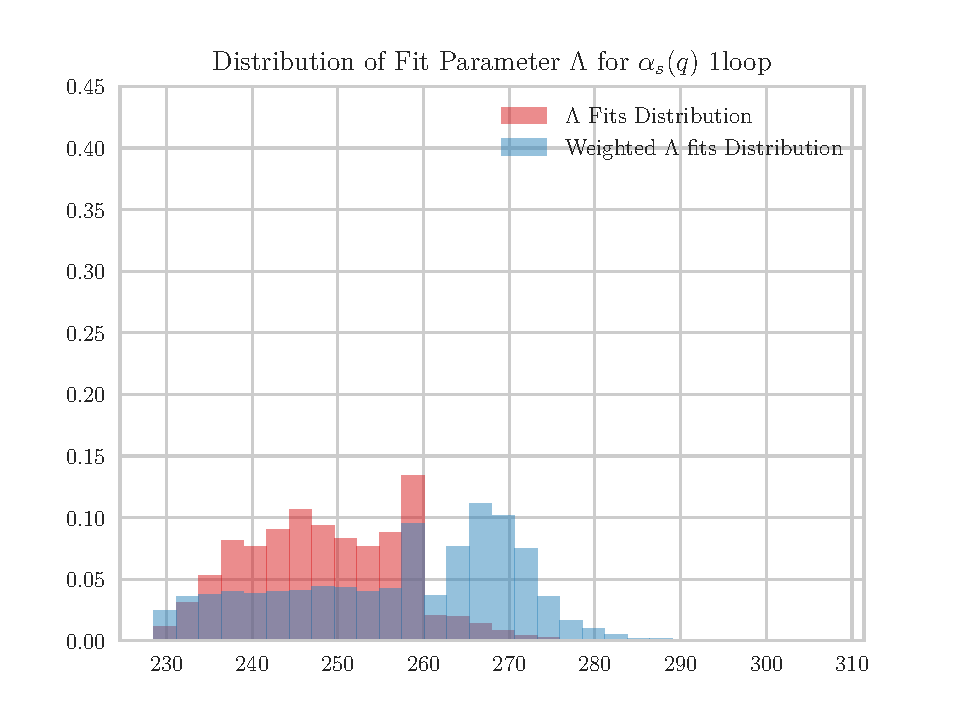
\includegraphics[width=1\textwidth]{results/hist1.pdf}
    \end{subfigure}
    \begin{subfigure}{0.49\textwidth}
        \centering
        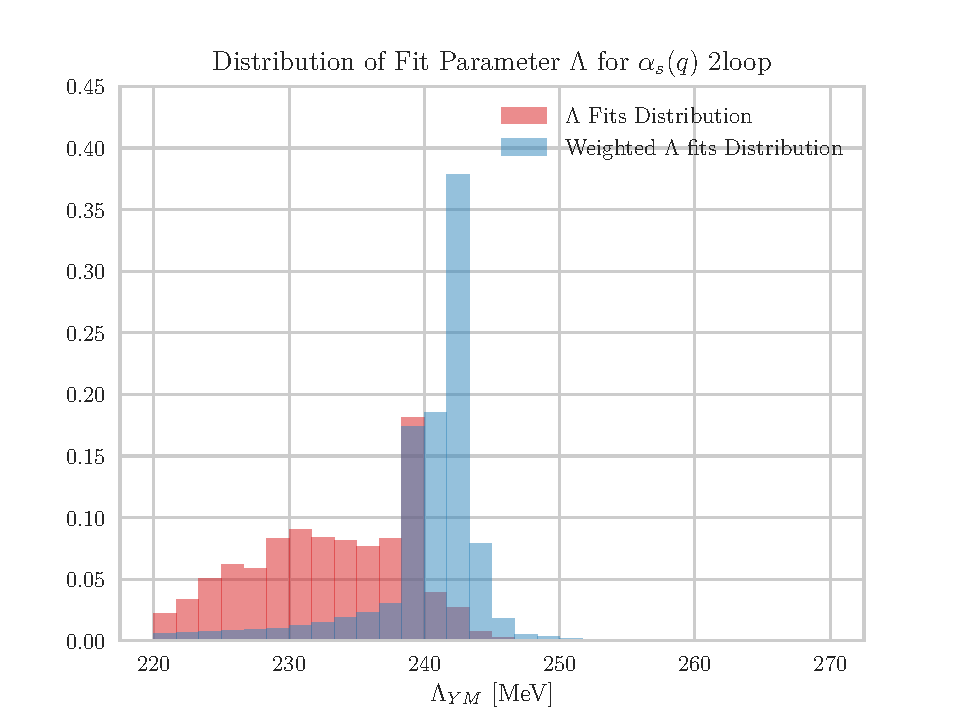
\includegraphics[width=1\textwidth]{results/hist2.pdf}
    \end{subfigure}

    \begin{subfigure}{0.49\textwidth}
        \centering
        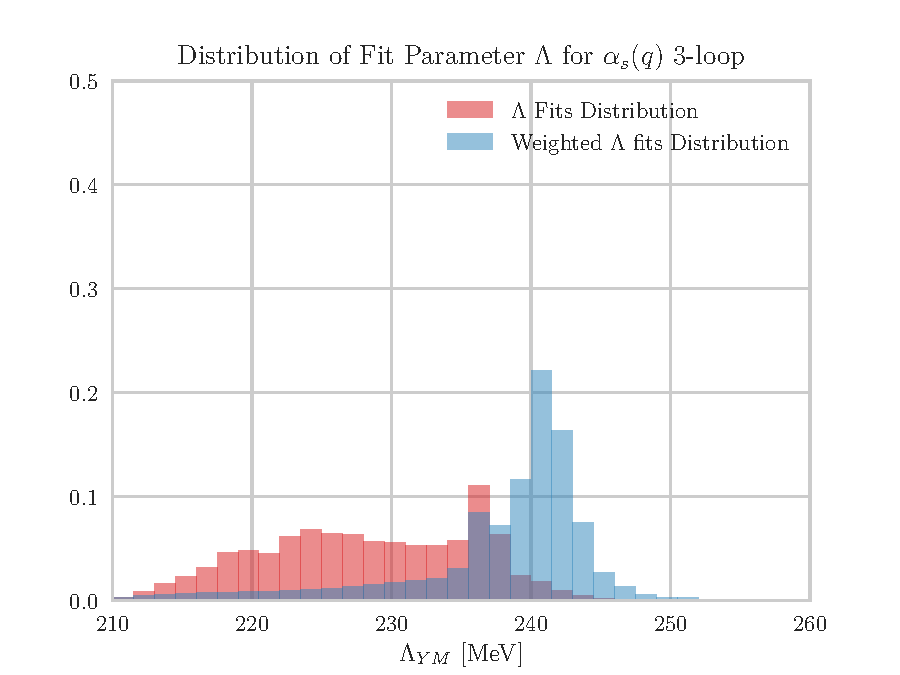
\includegraphics[width=1\textwidth]{results/hist3.pdf}
    \end{subfigure}
    \begin{subfigure}{0.49\textwidth}
        \centering
        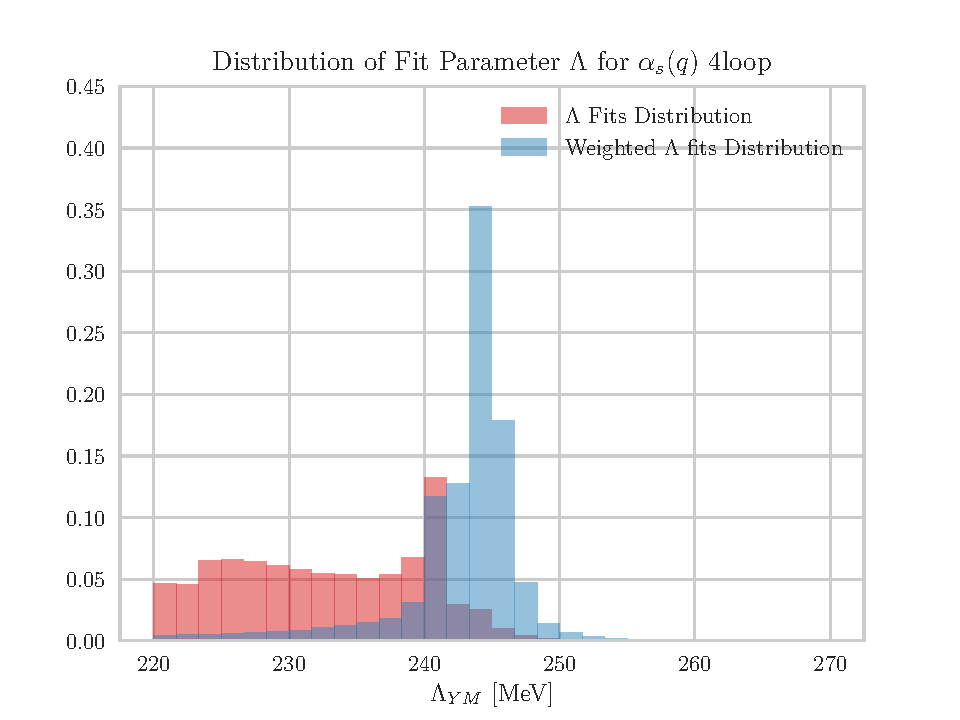
\includegraphics[width=1\textwidth]{results/hist4.pdf}        
    \end{subfigure}
    \caption{Normalized distributions of the fit parameters, $\Lambda$, obtained by all possible fit ranges between $t_f/r_0^2 = 0.005$ to $0.085$ of minimum size $0.005$. The four different plots are for the four different orders of corrections for $\alpha_s(q)$. Data for the distribution weighted with $1/\chi^2$, normalized to the number of fits, is also reported.}
    \label{lambda_hist}
\end{figure}

The fact that the weighted distributions have a peak means that there is a certain region in the energy spectrum where the function in \cref{eq:t2Ebuona} matches the data better. This is expected since we know that for low energies perturbation theory does not hold anymore, meaning that the function does not represent the data correctly. At high energies on the other hand, by looking at \cref{fig:t2EZoom} for example, the discretization effects introduced by the lattice method become relevant, so the continuum limit extrapolation that we made is unreliable in that region.\\
From the plot of the one-loop corrected function, one can see that there is no sharp peak in the weighted distribution compared to the others. The difference in the behavior is not surprising if one looks at \cref{fig:couplings} and considers that the higher order functions for $alpha_s(q)$ are all close together in the energy range considered. 

The estimation of the $\Lambda_{YM}$ scale is taken by considering the weighted median of the data, which is defined as the $50\%$ weighted percentile, the element $x_k$ of an ordered set of values $x_1, x_2, \dots, x_N$ that satisfies:
\beq
    \sum_{i=0}^{k-1} w_i \leq \frac{1}{2} ~~~~ \text{and}  ~~~~~ \sum_{i=k+1}^{N} w_i \geq \frac{1}{2}.
\eeq
The systematic uncertainty has been taken as the $68\%$ confidence interval of the weighted median distribution, as it was done in \cite{durr_ab-initio_2008-1}. To estimate the statistical error, the whole procedure has been applied to 500 bootstrap samples of the lattice data, constructing the continuum limit limit for each sample and performing fits on all fit ranges for sample. The results are shown in \cref{table:lambda_table}.

\begin{table}[!htb]
    \begin{center}
        \capt{Final results for the scale $\Lambda_{YM}$ from the distribution of the fits in \cref{lambda_hist}. The results are shown as $r_0\Lambda_{YM}$, the dimensionless lattice value for the scale. The value of  $\Lambda_{YM}$ in MeV is taken by setting $r_0=0.5$ fm. The first value within brackets after one value is the systematic error, given by the width of the weighted fit distribution. The second value within brackets is the statistical error, estimated by the standard deviation of the weighted means of the bootstrap samples.}
        \begin{tabular}{ccc} 
            Fit Function Order & $r_0\Lambda_{YM}$ & $\Lambda_{YM}$ [MeV] \\\hline
            1-loop & $0.656(78)(17)$ & $259(31)(7)$ \\
            2-loop & $0.612(26)(2)$ & $242(10)(1)$  \\
            3-loop & $0.608(38)(3)$ & $239(15)(2)$  \\
            4-loop & $0.618(32)(2)$ & $244(13)(1)$  
        \end{tabular}
        \label{table:lambda_table} 
    \end{center} 
\end{table}

The statistical error is consistently smaller than the systematic. This means that the weighted fitting procedure is not affected by statistical fluctuations and that the outcome of the fit is reliable. However the rate of the errors also implies that almost all the uncertainty is given by the method used to estimate $\Lambda_{YM}$. \\
Perhaps unsurprisingly, the result for the one-loop corrected form of $\alpha_S(q)$ differs significantly from the higher order corrections. The uncertainty is also by far larger. However, this difference is easily explained by considering \cref{fig:couplings}, which shows that the distance between the one-loop expression for $\alpha_S(q)$ is significantly different from all the others. 
The values we found for $\Lambda_{YM}$ can now be compared with the ones found in the literature for the same quantity using different methods. In particular we compare it with the one found in \cite{capitani_non-perturbative_1999} obtained using a recursive finite-size technique, which is reported as $\Lambda_{ref} = 238(18)$ MeV. The values found in \cref{table:lambda_table} agree very well with the reference.\\ 
One last result to show is the plot of $t_f^2\langle E\rangle$ as function of $q$ using the perturbative expression, \cref{eq:t2Ebuona}, and our values of $\Lambda_{YM}$ as input. In \cref{fig:end,fig:end1} the function is plotted for every order, together with the continuum limit data extrapolated from the lattice. We can see that good agreement is found between $q \approx 700$ and $1600$ MeV, or in flow time between $t_f/r_0^2 \approx 0.008$ to $t_f/r_0^2 \approx 0.045$

\begin{figure}[hbt!]
    \centering
    \begin{subfigure}{0.7\textwidth}
        \centering
        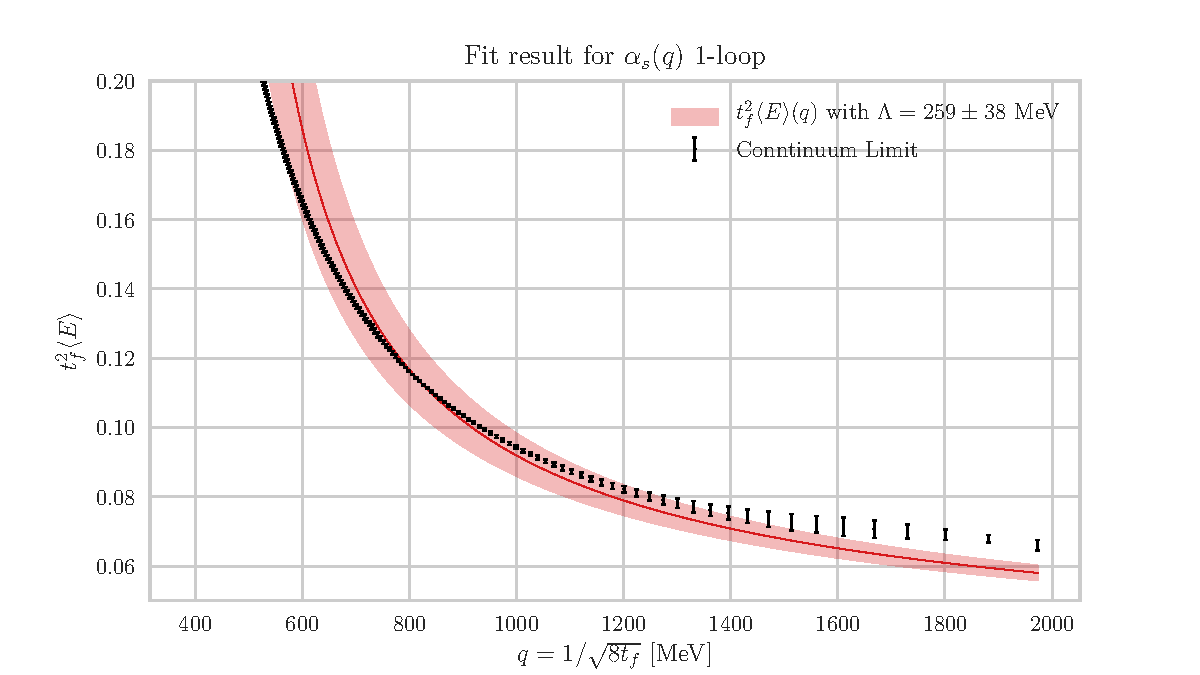
\includegraphics[width=1\textwidth]{results/End1.pdf}
    \end{subfigure}
    \begin{subfigure}{0.7\textwidth}
        \centering
        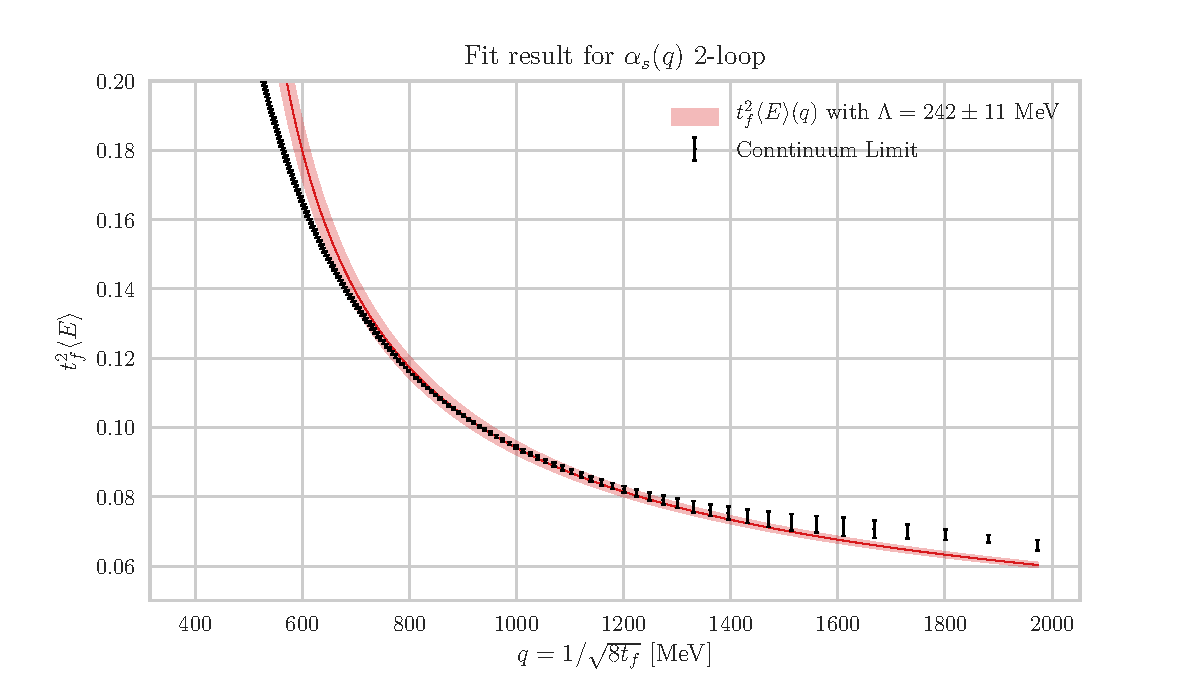
\includegraphics[width=1\textwidth]{results/End2.pdf}
    \end{subfigure}

    \caption{Plot of $t_f^2\langle E\rangle$, \cref{eq:t2Ebuona} as a function of the momentum scale $q$, using the values of the scale found in \cref{table:lambda_table}. The error band is the sum of the statistical and systematic errors from the same table. The data series in black is the continuum limit extrapolated from the lattice. On the top the function is plotted using the one-loop corrected expression for $\alpha_S(q)$ and $\Lambda_{YM} =259(31)(7)$ MeV. The bottom plot uses the two-loop corrected  $\alpha_S(q)$ and $\Lambda_{YM} =242(10)(1)$ MeV. Note that the plotted continuum function is the result of the multiple weighted fits procedure.}
    \label{fig:end}
\end{figure}
\begin{figure}[hbt!]
    \centering
    \begin{subfigure}{0.7\textwidth}
        \centering
        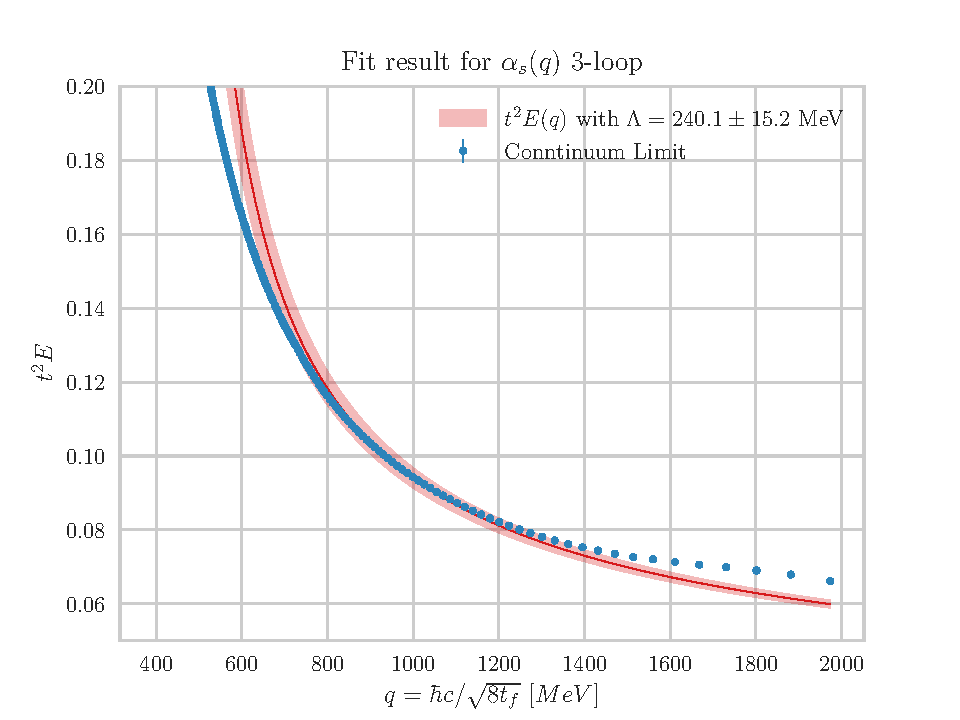
\includegraphics[width=1\textwidth]{results/End3.pdf}
    \end{subfigure}
    \begin{subfigure}{0.7\textwidth}
        \centering
        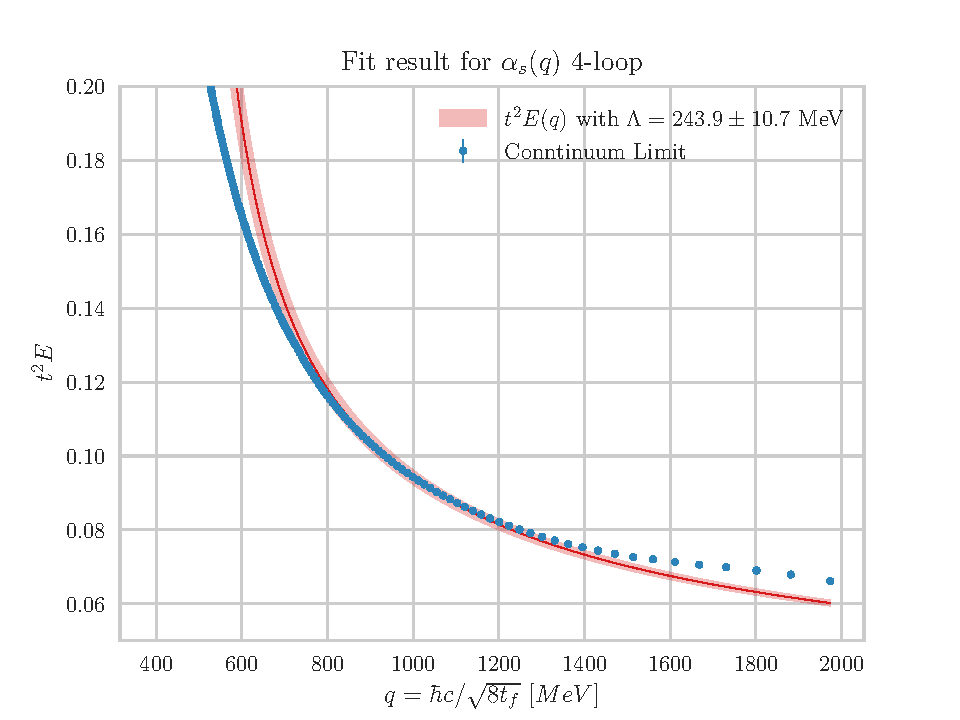
\includegraphics[width=1\textwidth]{results/End4.pdf}        
    \end{subfigure}
        \caption{Plot of $t_f^2\langle E\rangle$, \cref{eq:t2Ebuona} as a function of the momentum scale $q$, using the values of the scale found in \cref{table:lambda_table}. The error band is the sum of the statistical and systematic errors from the same table. The data series in black is the continuum limit extrapolated from the lattice. On the top the function is plotted using the three-loop corrected expression for $\alpha_S(q)$ and $\Lambda_{YM} =239(15)(2)$ MeV. The bottom plot uses the four-loop corrected  $\alpha_S(q)$ and $\Lambda_{YM} =244(13)(1)$ MeV. Note that the plotted continuum function is the result of the multiple weighted fits procedure.}
    \label{fig:end1}
\end{figure}

The conclusion we can make from these results is that there is clear agreement between the perturbative expansion in the coupling of $t_f^2\langle E\rangle$ and the continuum limit extrapolation that we performed for every flow time in the intermediate energy range. At low values of $q$, as expected,  the perturbative expansion diverges from the lattice data. As the coupling $\alpha_S(q)$ increases, perturbation theory becomes less accurate.\\
The more controversial data to interpret is the high-energy limit. In principle, once the continuum limit is recovered from the lattice data, the data should always be consistent with perturbation theory. However, we see that our continuum limit extrapolation is systematically higher than the results of our fitting procedure.  \\
One possible check of this would be to only consider the high-energy points in the fit. The resulting fit however, would be very far from the data at smaller energies. We performed this simple check by fitting only the values between $1.4$ and $2$ GeV. The value we found, in the case of four-loop-corrected $\alpha_S(q)$, is $r_0\Lambda_{YM} = 709(31)$ MeV, which is a much worse estimate for the quantity, also basing the comparison on reference \cite{capitani_non-perturbative_1999}. This is probably an indication that the high-energy mismatch is most likely a flaw of the continuum limit extrapolation. A possible issue is for example highlighted in \cref{fig:extrapolation005}, where one can see that the final extrapolated value is affected by systematic errors introduced by the choice of which lattice spacings to fit. In a more general picture, this means that a proper estimation of the systematics of the extrapolation at low flow times is needed in order to recover the correct continuum limit at high energies.\\
One further remark should be made on the procedure we used to find the best estimate of $\Lambda_{YM}$. The method of performing multiple fits over different windows of the momentum scale $q$ and the choice of weighting them with the fit quality, proved successful. In particular the assessment of the systematic uncertainty seems to be reasonable. A single fit over the whole energy range would have produced a very different result. However we expect the matching of the continuum limit data with the perturbative expansion of  $t_f^2\langle E\rangle$  to be better at high-energies, so a possible improvement could be to add some weights to the different fitting windows depending on their range, in order to give more importance to the fits performed at high $q$. 

  	\end{chapter}
\end{part}

% PART IV: CONCLUSIONS
\begin{part}{Conclusions}
	\label{part:conclusion}
	\begin{chapter}{Summary and Outlook}
		\label{chap:conclusion}
		The fact that the total uncertainty of our results is lower for the high order definitions of $\alpha_s(q)$ can be interpreted in two
	\end{chapter}
	
	% \begin{chapter}{Future Developements}
	% 	\label{chap:future}
	% 	\input{conclusion/future}
	% \end{chapter}
\end{part}


% APPENDICES
\begin{part}{Appendices}
	\begin{appendices}
		\begin{chapter}{Statistical Tools}
			\label{appendix:resampling}
			The determination of the uncertainty of the results of a numerical experiment is extremely important. In cases of small datasets, as in this work or in Lattice QCD in general, resampling methods are a popular solution for improving the estimate of the uncertainty. Another very important statistical property that is to be considered is the autocorrelation, introduced by the use of Markov chains.

\section{Resampling: Bootstrap and Jackknife}
Given a set of $N$ measurements of an observable $O$, a first estimate of the expectation value and of the uncertainty are the mean and the standard deviation of the data:
\beq
    \bar O = \frac{1}{N}\sum_{i=1}^N O_i, ~~~~~~ \sigma_O = \sqrt{\frac{1}{N}\sum_{i=1}^N (O_i - \bar O)^2},
\eeq
where $O_i$ are the measured values of the observable. Resampling methods use the data $O_i$ to construct multiple data series, and the average statistical properties of these series are used to estimate the properties of the original set. Both the bootstrap and the jackknife methods assume uncorrelated data. The observable $O$ can also be a derived quantity, such as a fit on some raw data.

\subsection{Bootstrap}
\label{app:resampling}
The Bootstrap method consists in building $N_b$ bootstrap samples by choosing $N$ points at random from the the original values (repetition are allowed). The average of a bootstrap sample is then:
\beq
    \hat O_b = \frac{1}{N}\sum_{i=1}^N O_{r(N)},
\eeq
where $r(N)$ stands for a random number between $1$ and $N$. One then has $N_b$ such averages and constructs:
\beq
    \tilde O = \frac{1}{N_b}\sum_{b=1}^{N_b} \hat O_b, ~~~~~~ \tilde\sigma_{\tilde O} = \sqrt{\frac{1}{N_b}\sum_{b=1}^{N_b} (O_b - \tilde O)^2}.
\eeq
The expectation value of the observable is then $\langle O \rangle = \tilde O$ and its associated uncertainty is $\tilde\sigma_{\tilde O}$.

\subsection{Jackknife}
The Jackknife sample are not constructed at random, as is the case for bootstrap, but in a systematic manner. One creates $N$ jackknife samples by removing for each of them the $j$th element of the data:
\beq
\hat O_j = \frac{1}{N-1}\sum_{i\neq j}^N O_i.
\eeq
One then computes:
\beq
\tilde O = \frac{1}{N}\sum_{j=1}^{N} \hat O_j, ~~~~~~ \tilde\sigma_{\tilde O} = \sqrt{\frac{N-1}{N}\sum_{j=1}^{N} (\hat O_j - \tilde O)^2}.
\eeq
The final estimator for the expectation value is  $\langle O \rangle = \tilde O$ and the uncertainty is $\tilde\sigma_{\tilde O}$.\\

Both of these resampling methods have been implemented and used; they were found to be consistent with each other. The jackknife is deterministic, the bootstrap, for sufficiently large $N_b$ (usually $\approx 500$ are sufficient) had error estimates compatible with jackknife and of the same order of magnitude. The error estimate when using resampling compared to the standard deviation is smaller by orders of magnitude.

\section{Autocorrelation}
\label{app:autocorr}
The data generated via a Markov chain Monte Carlo method is always affected by autocorrelation because the data points intrinsically depend on each other. One can tune the algorithm to reduce the autocorrelation time until it becomes negligible, but this is not the case for Lattice calculations because of the computational cost involved.\\
We followed the procedures in \cite{dewitt-morette_monte_1997} to get an algorithm to estimate the integrated autocorrelation time and the error correction factor due to autocorrelation. \\
The autocorrelation function of an ordered set variables $\{x_1, x_2,\dots x_N\}$ with expectation value $\bar x$ is defined as:
\beq
    \Gamma(t) = \Gamma(-t) = \langle (x_i - \bar x)(x_{i+t} - \bar x)\rangle \approx \frac{1}{N-t}\sum_{i=1}^{N-t}  (x_i - \bar x)(x_{i+t} - \bar x),
\eeq 
where $t$ is the ``lag'' between two points. The integrated autocorrelation time is given by:
\beq
    \tau_{int} = \frac{1}{2} \sum_{t=1}^\infty \frac{\Gamma(t)}{\Gamma(0)} = \frac{1}{2} \sum_{t=1}^\infty \rho(t).
    \label{autocorr:inf}
\eeq
For sufficiently large $N$, the true variance of the data can be expressed as:
\beq
    \tilde\sigma^2 = 2\tau_{int}\sigma^2 .
    \label{eq:tauint}
\eeq
This result is very neat, because it implies that in one can calculate the integrtated autocorrelation time correctly, the inclusion of the effects on the uncertainty estimate is trivial. In order to truncate the infinite summation in \cref{autocorr:inf} one can look at the deviation squared of $\rho(t)$, which as suggested by Sokal \cite{dewitt-morette_monte_1997} can be written as:
\beq
    \langle \delta \rho(t)^2\rangle \approx \frac{1}{N} \sum_{k=1}^\infty \left[ \rho(k+t) + \rho(k-t) - 2\rho(k)\rho(t)\right]^2.
\eeq
All these terms, for a sufficiently large value of $k$ should all vanish, hence one can choose a cutoff $\Lambda$ and truncate the sum up to $t+\Lambda$. The integrated autocorrelation time, if the deviations of $\rho(t)$ become small, plateaus, so one can truncate the sum in \cref{autocorr:inf} as well: 
\beq
    \tau_{int} = \frac{1}{2} \sum_{t=1}^W \rho(t),
    \label{autocorr_time}
\eeq
where $W$ is the first lag $t$ for which $\rho(t) < \sqrt{ (\langle \delta \rho(t)^2\rangle}$, when the contribution to the integration of $tau_{int}$ from that lag become smaller than the deviation of that same lag. \\
An approximate error estimate of the integrated autocorrelation time can be defined as:
\beq
    \sigma^2(\tau_{int}) \approx \frac{2(2W+1)}{N}\tau_{int}^2
    \label{eq:tauint_error}
\eeq

The integrated autocorrelation time has been computed for all quantities presented in this work and statistical uncertainties associated with results have all been corrected via \cref{eq:tauint}
		\end{chapter}
	\end{appendices}
\end{part}

% MAKE BIBLIOGRAPHY
\bibliographystyle{unsrt}
\bibliography{bibliography/master_thesis,bibliography/master_thesis_1}


\begin{acknowledgements}
	The conclusion of this master thesis marks the end of an amazing and very intense period of my life. My adventure in Norway has come to an end and a new beginning is opening in front of me. I feel like I ought to thank all the great people I have met and worked with in these three years. 

First I have to thank my two supervisors: Morten Hjorth-Jensen and Andrea Shindler. I want to express my deep admiration for the constant support and the endless inputs even if we were on two different continents. I really thank you for the opportunity you have given me and for the time spent at MSU together.

Then I want to thank Mathias Vege, for having shared this journey into Lattice QCD with me. I don't know how I would have done without the great discussions we had. I really enjoyed our adventure in Michigan and I hope we'll work again together in the future.

Next, I have to thank Alessio Pizzini. You know how much it meant to have someone to share this three years exploring Physics and Norway. 

I also have to thank Anders Johansson, my office mate. It's been great sharing with you the most random thoughts every day, together with the weirdest pieces of code we could find. Everything in between a game of Smash and the other.

A big thank you to all the Comp-Phys group at UiO. Spending my time with you has been amazing, no matter if it was on Physics, playing in the kitchen or talking about the most diverse issues. I loved spending my week-ends, evenings and nights at work because of you. I hope the spirit of this group will never be lost.

I cannot disentangle this work from all the other people that made my stay in Norway so nice. Thanks to Davide, Lorenzo and Federico, but also Giulio and Mattia. You guys have been amazing. Thanks also to Jan, Diane and Marie, because our friendship has been something special for me. And thanks to all the other great people I have met here.

Then to my parents, because they filled me with curiosity, inspired me and made me who I am. For the unconditional support you've given me. Regardless of the distance you always help me.

And finally to you two, because no matter where life is taking us, you are the people I care about the most.

\vspace{2cm}
\begin{flushright}
    Oslo, 14th May 2018\\
    Giovanni Pederiva    
\end{flushright}





\end{acknowledgements}

% AND SO WE END
\end{document}
